% !TeX root = DCN.tex
\documentclass[twocolumn, aps, amsmath, amssymb, nofootinbib, superscriptaddress, longbibliography, floatfix, eqsecnum, rmp]{revtex4-2}

\usepackage[pdftex]{graphicx}
\usepackage{mathrsfs}
\usepackage[colorlinks, breaklinks, urlcolor={blue}, linkcolor={red}, citecolor={blue}]{hyperref}
% \usepackage{amsmath}
\usepackage{mathtools}
\usepackage[english]{babel}
\usepackage{booktabs}
% \usepackage{amssymb}
\usepackage{type1cm}
\usepackage{caption}
\usepackage{url}
\usepackage[breaklinks]{hyperref}
\usepackage{braket}
\usepackage{algorithm}
\usepackage{algpseudocodex}
\usepackage[strict]{changepage}
\usepackage{tikz}
\usepackage{pgfplots}

\pgfplotsset{compat=newest}

\usetikzlibrary{positioning, fit, calc, shadows, shadows.blur, arrows.meta, shapes.geometric}

\let\oldalgorithmic\algorithmic
\let\endoldalgorithmic\endalgorithmic

\renewenvironment{algorithmic}
{\begin{adjustwidth}{-1em}{}\oldalgorithmic}
{\endoldalgorithmic\end{adjustwidth}}

\frenchspacing
    
\captionsetup[figure]{margin=0pt, font=small, labelfont=bf, labelsep=endash, justification=centerlast, labelsep=colon}
\captionsetup[algorithm]{margin=0pt, font=small, labelfont=bf, labelsep=endash, justification=centerlast, labelsep=colon}
    
\begin{document}

\title{Distributed consensus networks}

\author{Peter P. Rohde}
\email[]{peter@peterrohde.org}
\homepage{https://www.peterrohde.org}
\affiliation{\mbox{BTQ Technologies, 16-104 555 Burrard Street, Vancouver BC, V7X 1M8 Canada}}
\affiliation{\mbox{Center for Engineered Quantum Systems, School of Mathematical \& Physical Sciences}, \mbox{Macquarie University, NSW 2109, Australia}}
\affiliation{\mbox{Hearne Institute for Theoretical Physics, Department of Physics \& Astronomy}, \mbox{Louisiana State University, Baton Rouge LA, United States}}

\begin{abstract}
Blockchains rely on distributed consensus algorithms to decide whether a proposed transaction is valid and should be added to the blockchain. The purpose of consensus is to act as an independent arbiter for transactions, robust against adversarial manipulation. This can be achieved by choosing random subsets of nodes to form consensus sets. In an economy where consensus is the commodity, consensus must be secure, computationally efficient, fast and cheap. Most current blockchains operate in the context of open networks, where algorithms such as proof-of-work are highly inefficient and resource-intensive, presenting long-term scalability issues. Inefficient solutions to allocating consensus sets equates to high transaction costs and slow transaction times. Closed networks of known nodes afford more efficient and robust solutions. We describe a secure distributed algorithm for solving the random subset problem in networks of known nodes, bidding to participate in consensus for which they are rewarded, where the randomness of set allocation cannot be compromised unless all nodes collude. Unlike proof-of-work, the algorithm allocates all nodes to consensus sets, ensuring full resource utilisation, and is highly efficient. While the protocol is synchronous, a staking mechanism ensures self-synchronisation with no dependence on an external reference. The protocol follows self-enforcing where adversarial behaviour only results in self-exclusion. Signature-sets produced by the protocol act as timestamped, cryptographic proofs-of-consensus, a commodity with market-determined value. The protocol is highly strategically robust against collusive adversaries, affording subnetworks defence against denial-of-service and majority takeover.
\end{abstract}

\maketitle

\tableofcontents

\section{Introduction}

Decentralised finance (DeFi) is the longstanding vision of a truly global and borderless financial system, the promise of universal, low-cost access to banking services and international financial markets, eliminating geographic and socio-political barriers of entry and reliance upon centralised financial institutions, subverting the power-base of monopolistic and hegemonic access to capital, facilitating a highly competitive global economic landscape.

Smart-contracts enabling arbitrary, self-executing algorithmic exchange facilitate the synthesis of sophisticated financial instruments in the absence of conventional centralised exchanges. The algorithmic versatility of smart-contracts affords their use as a primitive in the construction of sophisticated distributed protocols such as Decentralised Autonomous Organisations (DAOs).

%The key characteristics of DeFi are \cite{???,EthereumDevs}:
%\begin{itemize}
%	\item Non-custodial: users assert full control over their own assets.
%	\item Open: protocols are borderless and globally accessible.
%	\item Transparency: protocols and algorithms are open-source.
%	\item Composable: code may be modularised and layered, enabling thriving development and innovation of the ecosystem.
%	\item Decentralised: the absence of top-down control and centralisation of power.
%\end{itemize}

In a decentralised environment transactions are approved via \emph{consensus} (Sec.~\ref{sec:consensus}) whereby a small number of randomly chosen network nodes (\emph{consensus sets}) collectively act as delegates for the network to authorise transactions. Consensus outcomes should with high probability reflect honest outcomes, a function of consensus set size and the ratio of dishonest nodes.

The randomisation of nodes forming consensus is vital to ensure the integrity of consensus outcomes (Sec.~\ref{sec:random_subset_problem}). If the choice of consensus nodes were known in advance this would provide avenues for malicious parties to compromise security by targeting the known allocation. Randomisation effectively erases all assignment information of consensus node assignment, eliminating all avenues for strategic alignment.

The Bitcoin protocol \cite{Nakamoto08} first introduced proof-of-work (PoW) as mechanism for securely randomly selecting a small number of network nodes at random to form consensus (Sec.~\ref{sec:PoW}). This protocol operates in the context of a network of unknown and unidentifiable nodes in which anyone may freely participate. The algorithm requires nodes to compete to solve inverse-hashing problems, a randomised algorithm that effectively chooses winners by lottery.

While the proof-of-work mining algorithm provides an ingenious solution to the random subset problem it is highly inefficient, resulting in enormous net energy consumption to maintain the network. Currently, annualised energy consumption of the Bitcoin network is $\sim$155TWh \cite{CBECI}\footnote{Estimate as of January 19, 2024.}, comparable to the total electricity consumption of medium sized countries\footnote{Estimated annual electricity consumption of Sweden (2022): $\sim$164TWh.}.

The inefficiency of proof-of-work presents a significant obstacle for scalability, motivating the development of more efficient alternate consensus algorithms. Proof-of-stake (PoS) \cite{KingNadal, Bentov} is a leading alternative, recently adopted by the Ethereum network to improve scalability and reduce transaction costs. Ethereum's transition to proof-of-stake, famously known as \emph{The Merge}, reduced its annualised energy consumption from $\sim$21TWh (PoW) to $\sim$2GWh (PoS) \cite{CBECI}\footnote{Estimates immediately prior and subsequent to \emph{The Merge} on September 15, 2022.}, a spontaneous reduction in energy consumption of 99.99\%. However, despite its radically improved energy efficiency, proof-of-stake has been criticised for affording reduced security owing to its increased vulnerability to manipulation and reduced level of randomisation. Proof-of-work based on quantum sampling problems has also been investigated as a means for enhanced energy efficiency \cite{QPoW}.

Networks comprising known nodes afford more efficient distributed algorithms for solving the random subset problem. By utilising secure shared randomness (Sec.~\ref{sec:secure_shared_randomness}) all network nodes may be simultaneously allocated to random subsets (Sec.~\ref{sec:hash_based_random_subsets}), ensuring full resource utilisation.

The generalisation of the random subset problem is the \emph{consensus assignment problem} (Sec.~\ref{sec:consensus_assignment_problem}), enabling the simultaneous allocation of network nodes to arbitrary sets of consensus sets under asymmetric load.

\emph{Distributed consensus networks} (DCNs) combine the consensus assignment problem with an economic model that self-incentivises the honest participation of nodes (Sec.~\ref{sec:DCN}). The product of DCNs is proofs-of-consensus (PoC) --- timestamped, cryptographic proofs that a sets of nodes form secure random subsets of a network established via distributed execution of the consensus assignment problem (Sec.~\ref{sec:PoC}).

DCNs treat consensus as an abstract market commodity, an enabler of generic digital trade. The internal operation of DCNs is inherently non-monetary, a barter economy in which nodes contribute to consensus load in equal exchange for the consensus load they request. Nodes act as gateways to the DCNs to which they belong, and may independently utilise and monetise consensus load, collectively facilitating an externally-facing competitive bidding market for consensus (Sec.~\ref{sec:economics}).

\emph{Quantum consensus networks} (QCNs) (Sec.~\ref{sec:QCN}) have quantum-enabled nodes, possessing quantum computational or communications resources, acting as secure, certifiable quantum random number generators (QRNGs) upon forming consensus, a commodity with market value. Other (classical) DCNs may observe QCNs as oracles, utilising their random bitstreams to add entropy (Sec.~\ref{sec:entropy_add}) to their own global keys, enabling quantum-random consensus assignment.

Existing blockchain design philosophy couples cryptocurrencies with the technological implementation of their mechanism for trade, a vertically integrated paradigm which frustrates inter-ledger exchange (Sec.~\ref{sec:conclusion}). The hard-wiring of currencies with specific consensus algorithms couples their cost of execution with monetary dynamics. The abstract separation between currencies and their mechanism for trade enables horizontal competition between currencies, likewise between competitors offering consensus as a commodity.

%??? TO DO
%
%Sec.~\ref{sec:applications}
%
%* Detached from specific 
%
%Sec.~\ref{sec:strategic_cons}

%Bitcoin is distributed but makes no assurances on decentralisation.
%https://www.bis.org/publ/qtrpdf/r_qt2112b.htm
%https://www.nber.org/system/files/working_papers/w29396/w29396.pdf#page47

%\cite{Schneier96}
  
\section{Consensus} \label{sec:consensus}

The purpose of consensus is to provide a decentralised mechanism for sets of parties to collectively act as an independent arbiter in judging and signing off on the validity of statements. In the context of blockchains, this is employed to determine whether a newly submitted transaction block is legitimate and should be added to the blockchain.

In an environment where a minority subset of parties are dishonest and conspiring to form false consensus, the purpose of consensus protocols is to uphold the will of the majority, independent of the behaviour of collusive, dishonest parties. As dishonest parties are assumed to be in the minority, this can always be achieved by ensuring that all parties are involved in consensus. However, this is highly resource-intensive and consensus needn't involve all parties. A subset of parties suffices to form consensus if their decision reflects the will of the majority, enabling them to act as delegates.

Choosing a subset of parties to form consensus there is some probability of dishonest parties forming a false majority by chance. Consensus sets should therefore be chosen to upper-bound this probability, independent of the strategy employed by dishonest parties.

Consensus is formed by majority vote on the validity of some statement (\texttt{id}) by members of a consensus set ($\mathcal{C}$) chosen from a set of network nodes ($\mathcal{N}$),
\begin{align}
	\mathcal{C}\subseteq\mathcal{N}.
\end{align}
The majority vote of the entire network is a deterministic decision function defining the \emph{source of truth},
\begin{align} \label{eq:majority_vote_det}
	\textsc{MajorityVote}(\mathcal{N},\mathtt{id})\to\{0,1\},
\end{align}
which consensus sets must uphold. Based on their statistical composition, the majority votes of consensus sets are in general probabilistic, 
\begin{widetext}
	\begin{align*}
	\textsc{MajorityVote}(\mathcal{C},\mathtt{id}) = \begin{cases}
        \mathrm{Pr}(1-P_c), & \textsc{MajorityVote}(\mathcal{N}, \mathtt{id}) \\
        \mathrm{Pr}(P_c), & \neg \textsc{MajorityVote}(\mathcal{N}, \mathtt{id})
    \end{cases},
	\end{align*}
\end{widetext}
where $P_c$ is the probability of compromise, whereby $\mathcal{C}$ comprises a majority of dishonest parties attempting to subvert honest outcomes.

For \mbox{$P_c=0$} where an honest majority is guaranteed, this reduces to the deterministic case as per Eq.~\eqref{eq:majority_vote_det}. The purpose of distributed consensus algorithms is to choose consensus sets $\mathcal{C}$ operating in this regime to a close approximation.

%\begin{algorithm}[!htb]
%\begin{algorithmic}
%\Function{Consensus}{$\mathcal{C}$, \texttt{statement}} $\to \{0,1\}$
%	\State \Return{\textsc{MajorityVote}($\mathcal{C}$, $\mathtt{statement})$}
%\EndFunction
%\State
%\Function{ConsensusTime}{$\mathcal{C}$} $\to \mathbb{R}$
%	\State \Return \textsc{Median}($\textsc{ReportedTimes}(\mathcal{C})$)
%\EndFunction
%\State
%\Function{ConsensusParticipants}{$\mathcal{C}$, $\mathcal{S}$} $\to \mathcal{P}$
%\State $\mathcal{P} = \{\}$ \Comment{Participant set}
%\For{$i\in\mathcal{S}$}
%	\If{\textsc{MajorityVote}($\mathcal{C}$, $\mathcal{S}_i\in\mathcal{P}$)}
%	\State $\mathcal{P} \gets \mathcal{P} \cup \mathcal{S}_i$
%	\EndIf
%\EndFor
%	\State \Return{$\mathcal{P}$}
%\EndFunction
%\end{algorithmic}	
%\caption{Consensus methods.} \label{alg:compliance}
%\end{algorithm}

\section{Random subset problem} \label{sec:random_subset_problem}

The \emph{random subset problem} is to choose a random subset $A$ uniformly from $B$, where $A\subseteq B$, of which there are $\binom{|B|}{|A|}$ combinations. If the proportion of parties acting dishonestly and collusively is $r$, the probability a random subset of size $N$ contains at least $k$ dishonest parties is,
\begin{align}
P(N,k,r) &= \sum_{n=k}^{N} \binom{N}{n} {r}^n (1-r)^{N-n} \nonumber\\
%	&= 1 - I_{1-r}(N-k+1,k) \nonumber\\
	&= I_r(k,N-k+1),
\end{align}
where $I_x(a,b)$ is the regularised incomplete beta function. Compromising vote integrity via false-majority requires,
\begin{align}
	k_\mathrm{maj} = \lfloor N/2 \rfloor + 1.
\end{align}
Hence, the likelihood of compromise is,
\begin{align}
	P_c(N,r) = I_r(\lfloor N/2 \rfloor + 1,N-\lfloor N/2 \rfloor).
\end{align}

While in principle all parties are associated with independent likelihood of compromise, $r_i$, choosing subsets uniformly at random ensures the probabilities of set members being dishonest are independently and identically sampled with the average-case probability $r$,
\begin{align} \label{eq:av_r_uniform}
	r = \frac{1}{|\mathcal{N}|} \sum_{i=1}^{|\mathcal{N}|} r_i.
\end{align}
Hence, $P_c$ is independent of how dishonest nodes are distributed and what strategies they might employ (Fig.~\ref{fig:strategy_entropy}).

\begin{figure}[!htb]
	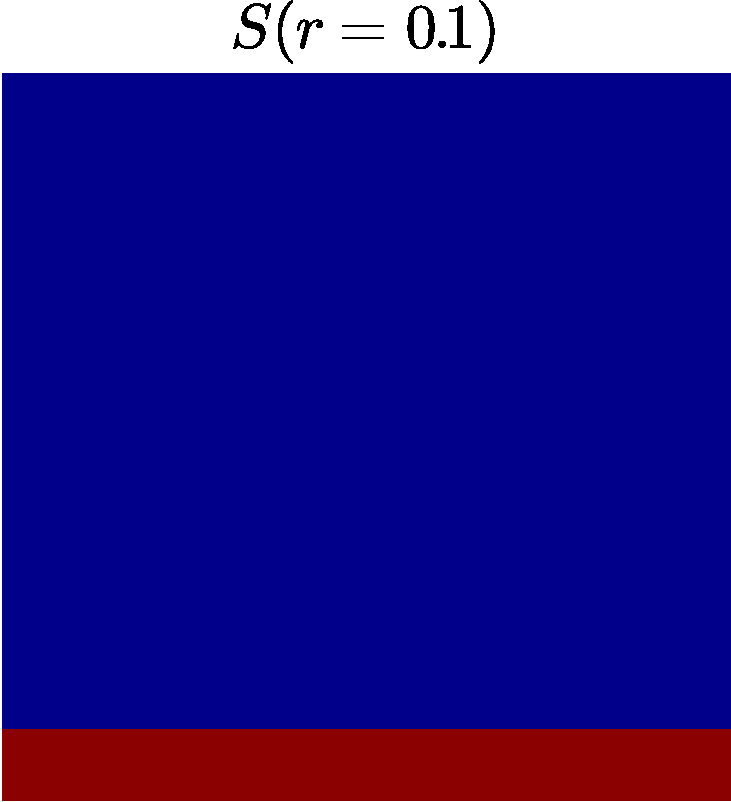
\includegraphics[width=0.49\columnwidth]{figures/strategy_entropy_S_r01.pdf}
	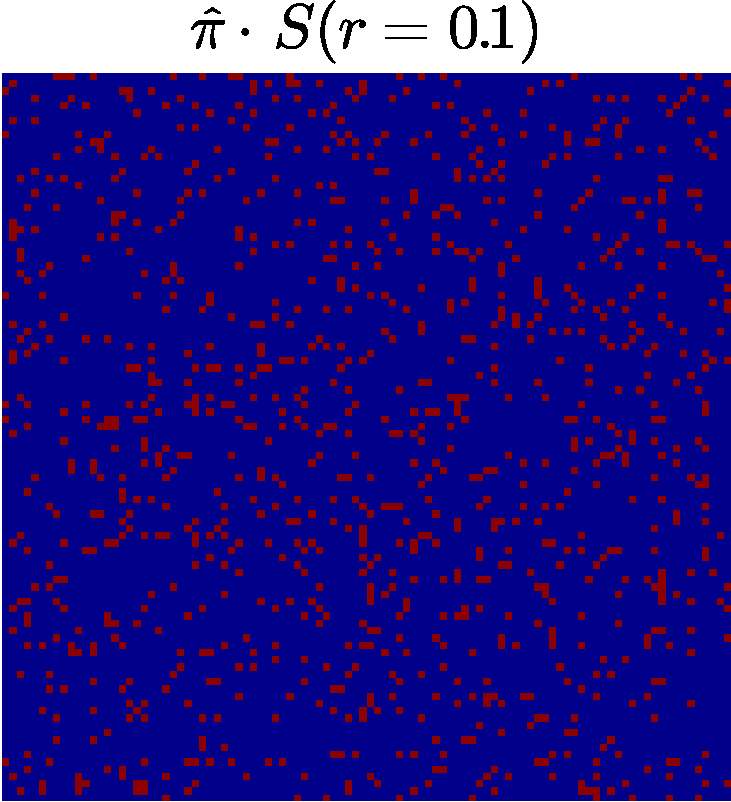
\includegraphics[width=0.49\columnwidth]{figures/strategy_entropy_R_r01.pdf}\\
	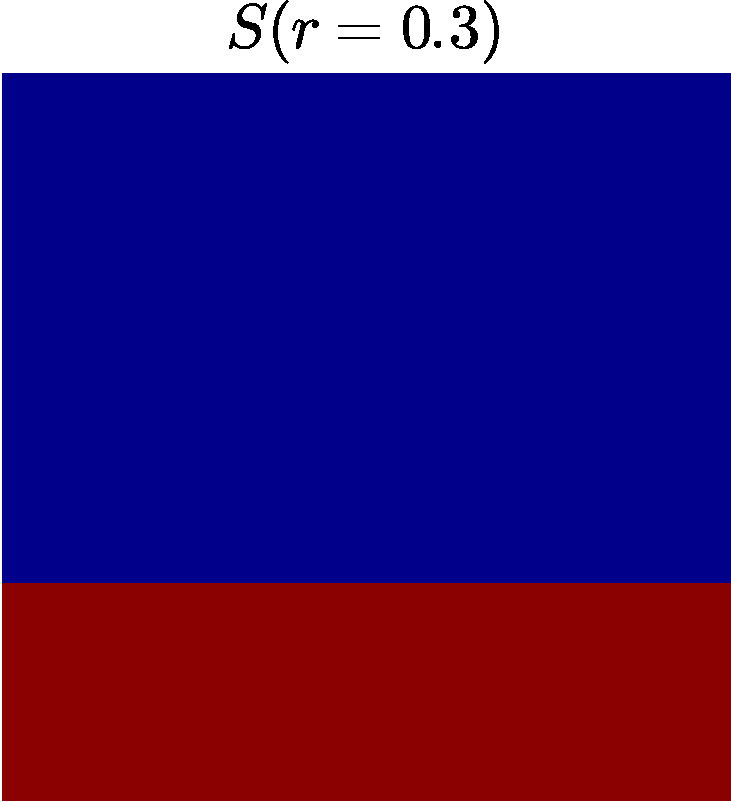
\includegraphics[width=0.49\columnwidth]{figures/strategy_entropy_S_r03.pdf}
	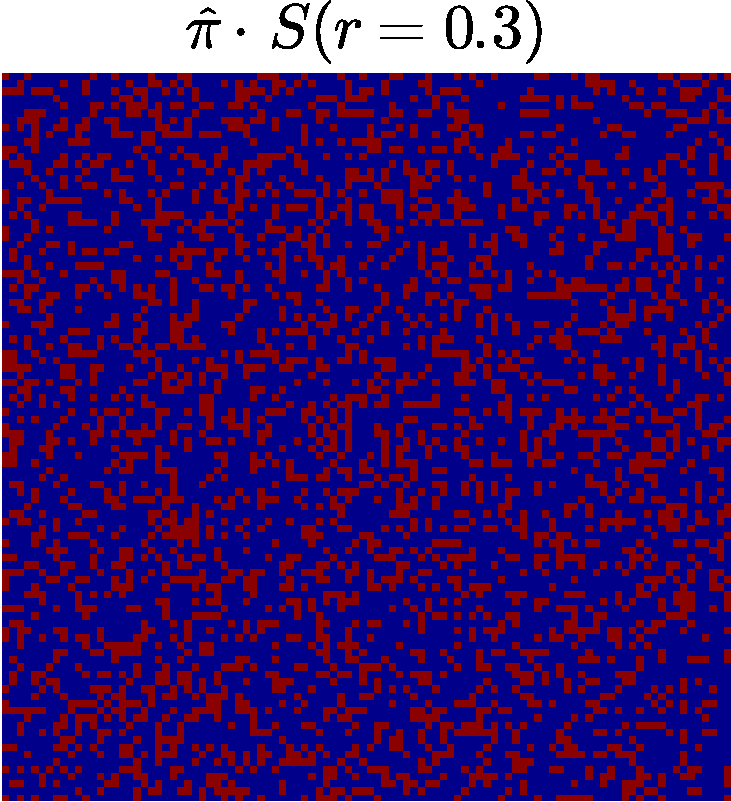
\includegraphics[width=0.49\columnwidth]{figures/strategy_entropy_R_r03.pdf}
	\caption{\textbf{Random sampling as a defence against strategic alignment.} (left) A minority of strategically aligned nodes may form false-majority if their alignment overlaps with a known allocation for consensus sets. (right) Random sampling erases strategic alignment and ensures node honesty is sampled with average-case $r$.} \label{fig:strategy_entropy}
\end{figure}

To uphold the integrity of majority votes, we require the likelihood of a minority gaining false-majority by chance to be upper-bounded by an exponentially small threshold $\varepsilon = 2^{-\lambda}$,
\begin{align}
	P_c(N,r) &\leq\varepsilon,
\end{align}
for statistical security parameter $\lambda>1$, a subjective parameter which may be application- or user-dependent. %As more stringent $\varepsilon$ implies larger $N_C$ hence workload, the cost of consensus is parameterised by $\varepsilon$.

We define the required consensus set size, $N_\mathrm{min}$, as the smallest set size satisfying this inequality,
\begin{align}
	N_\mathrm{min}(r,\varepsilon) &= \underset{N\in\mathbb{Z}^+}{\arg\min}(P_c(N,r)\leq\varepsilon).	
\end{align}

For consensus to maintain $\varepsilon$-security, consensus sets should never be smaller than $N_\mathrm{min}$. Simultaneously, choosing consensus sets larger than $N_\mathrm{min}$ is unnecessary and wasteful. Tradeoff curves for $N_\mathrm{min}(r,\varepsilon)$ are shown in Fig.~\ref{fig:P_M}.

%\footnote{The number of distinct partitions of a set of nodes $\mathcal{S}$ into consensus sets of sizes $\{|\mathcal{C}_i|\}$ where,
%\begin{align}
%		|\mathcal{S}| = \sum_i |\mathcal{C}_i|,
%\end{align}
%is given by,
%\begin{align}
%	\# = \prod_i \binom{|\mathcal{S}|-\sum_{j=1}^{i-1}|\mathcal{C}_j|}{|\mathcal{C}_i|}.
%\end{align}
%}

\begin{figure}
	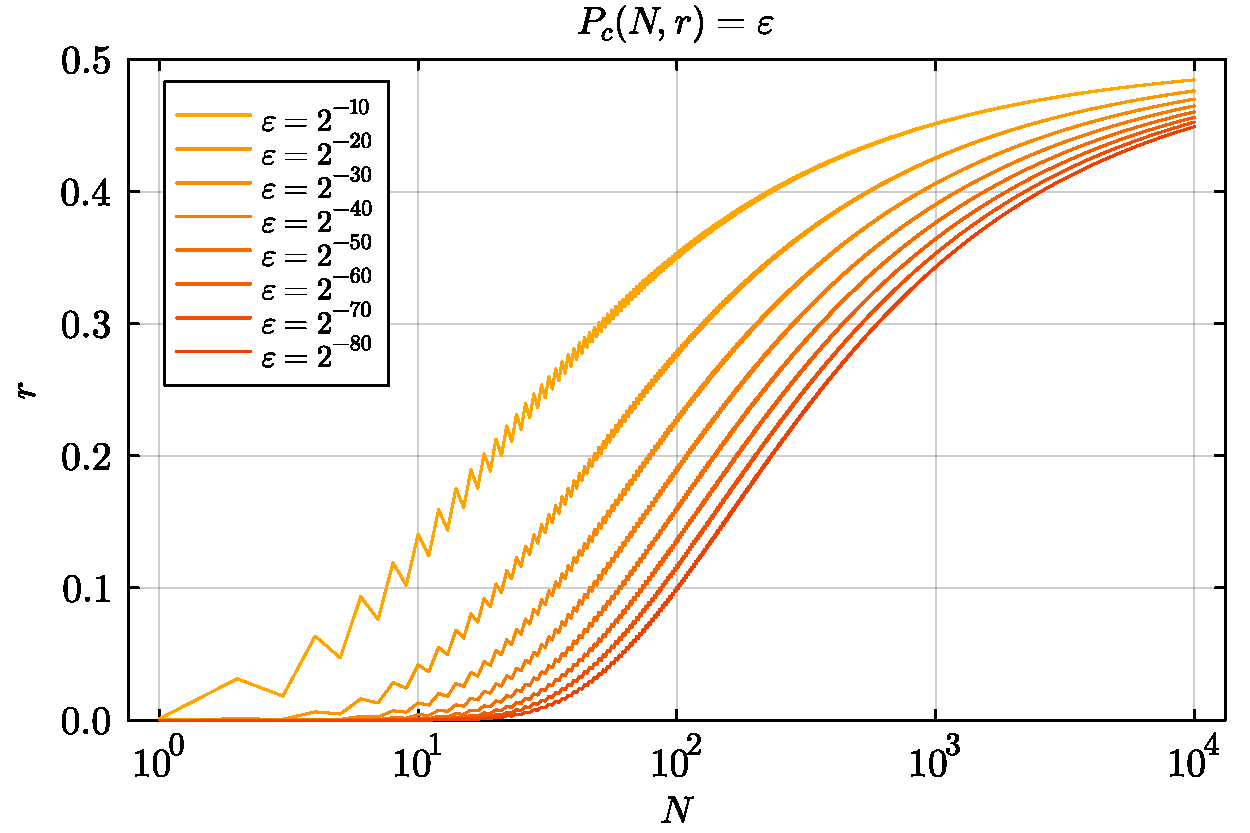
\includegraphics[width=\columnwidth]{figures/majority_prob.pdf}\\
	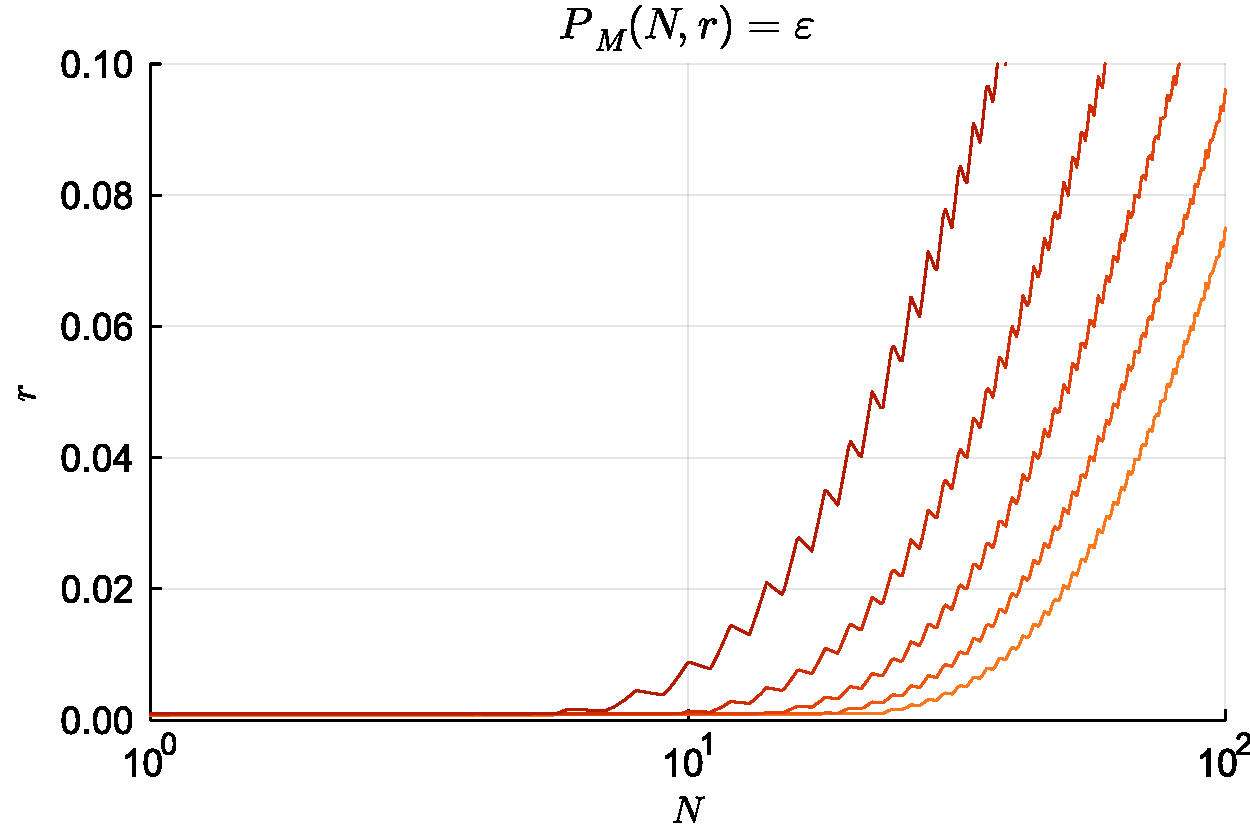
\includegraphics[width=\columnwidth]{figures/majority_prob_zoom.pdf}
	\caption{\textbf{Security tradeoffs with consensus set size.} $P_c(N,r)\leq\varepsilon$ is the probability that dishonest nodes within a random subset of size $N$ form a false-majority when the proportion of dishonest nodes is $r$, where $\varepsilon=2^{-\lambda}$ is the statistical security parameter. The oscillatory artefacts are associated with the non-linearity of \mbox{$\lfloor N/2\rfloor$} for even- and odd-valued $N$.} \label{fig:P_M}
\end{figure}

\subsection{Centralised algorithm}

The random subset problem has a trivial centralised solution (Alg.~\ref{alg:random_subset}). We assign unique random bit-strings to each node, order them by their random number, and partition the ordered list piecewise into units of length $N_\mathrm{min}$. These partitions form non-intersecting random subsets, each defining an independent consensus set.

\begin{algorithm}[H]
\begin{algorithmic}
\Function{RandomSubsets}{$\mathcal{S}$, $\{|\mathcal{C}|\}$} $\to \{\mathcal{C}\}$
	\LComment{Assign a random number to each node}
	\For{$i\in\mathcal{S}$}
		\State $\mathtt{random}_i \gets \textsc{Random}(\{0,1\}^n)$	\EndFor
	\LComment{Sort nodes by their random number}
	\State{$\mathtt{ordered}$ = \textsc{Sort}($\mathcal{S}$, $\mathtt{random}$)}
	\LComment{Partition the list into consensus sets}
	\State{$\{\mathcal{C}\}$ = \textsc{Partition}(\texttt{ordered}, $\{|\mathcal{C}|\}$)}
	\State \Return{$\{\mathcal{C}\}$}
\EndFunction
\end{algorithmic}
\caption{Centralised algorithm for the random subset problem, assigning a set of nodes $\mathcal{S}$ to a set of independent random subsets $\{\mathcal{C}\}$ of given sizes $\{|\mathcal{C}|\}$.} \label{alg:random_subset}
\end{algorithm}

The challenge is to securely implement this algorithm in a decentralised environment, such that nodes are unable to compromise the randomness of the assignments of consensus sets.

\subsection{Proof-of-work} \label{sec:PoW}

* Hashcash: \cite{pow_email, hashcash}

Proof-of-work has been widely employed in blockchains such as Bitcoin \cite{Nakamoto08} as a distributed protocol for choosing random subsets of nodes. Here, nodes compete to find satisfying inputs to hash functions whose outputs satisfy a constraint dictating the likelihood of success. This distributed algorithm effectively asks nodes to find solutions to randomised problems with very low probability of success, $p_\mathrm{mine}\ll 1$, such that winners are randomly allocated across nodes in the network.

Since hash functions are pseudo-random and exhibit pre-image resistance\footnote{For $\textsc{Hash}(x)\to y$ it is computationally hard to find a satisfying input $x\in\{0,1\}^*$ for given output $y\in\{0,1\}^n$.}, the only viable approach to finding such solutions is via brute-force, repeatedly hashing random bit-strings until a satisfying input is found. Winning nodes are hence allocated at random and cannot be spoofed under a computational hardness assumption. The distributed algorithm for proof-of-work is shown in Alg.~\ref{alg:PoW}.

\begin{algorithm}[H]
\begin{algorithmic}
\Function{ProofOfWork}{$\mathcal{S}$, \texttt{id}, \texttt{size}} $\to \mathcal{C}$
	\State $\mathcal{C} = \{\}$ \Comment{Consensus set}
	\While{$|\mathcal{C}|<\mathtt{size}$}
	\For{$i\in\mathcal{N}$} \Comment{In parallel}
		\State $\mathtt{random}_i = \textsc{Random}(\{0,1\}^n)$
		\State $\mathtt{output}_i = \textsc{Hash}(\mathtt{id}\,|\,\mathtt{random}_i)$
		\If{$\textsc{Valid}(\mathtt{output}_i)$}
			\State $\mathcal{C} \gets \mathcal{C} \cup \mathcal{S}_i$
		\EndIf
	\EndFor
	\EndWhile
	\State \Return{$\mathcal{C}$}
\EndFunction
\State
\Function{Valid}{$x\in\{0,1\}^n$} $\to \{0,1\}$
	\If{$x/2^n \leq p_\mathrm{mine}$}
		\State \Return{\texttt{true}}
	\Else
		\State \Return{\texttt{false}}
	\EndIf
\EndFunction
\end{algorithmic}
\caption{Random subsets via proof-of-work. Nodes $\mathcal{S}$ hash random bit-strings, salted by a problem instance specified by the previous block $\mathtt{id}$, where the per-hash success rate is $p_\mathrm{mine}$.} \label{alg:PoW}
\end{algorithm}

Proof-of-work has no requirement that nodes be known or trusted, providing a very general protocol suited to open networks in which anyone can participate. However, while affording a distributed solution to the random subset problem, this approach is inherently wasteful. The expected mining rate is,
\begin{align}
	R_\mathrm{mine} = p_\mathrm{mine}\cdot R_\mathrm{hash},
\end{align}
where $R_\mathrm{hash}$ is the network's net hash-rate\footnote{Bitcoin's cumulative network hash-rate was $\sim$500EH/s \mbox{($500\times 10^{18}\mathrm{H/s}$)} as of January, 2024 \cite{hash_rate}.}. To inhibit the formation of multiple, simultaneous consensus sets (double-mining), potentially manifesting itself as forks in the blockchain, proof-of-work systems may introduce \emph{friction} by algorithmically adjusting the \emph{difficulty parameter} to ensure consistent mining times. To achieve constant mining time, difficulty must scale with cumulative network hash-rate, making the distributed algorithm less efficient as network size grows. For example, maintaining constant mining rate implies efficiency scales inversely with network size,
\begin{align}
	p_\mathrm{waste}=1-O\left(\frac{1}{n}\right),
\end{align}
asymptotically perfectly inefficient.

\subsection{Secure shared randomness} \label{sec:secure_shared_randomness}

An environment comprising a network of known nodes affords a more efficient solution to the random subset problem. The key observation is to utilise  \emph{secure shared randomness} to randomly permute and partition sets of nodes as per Alg.~\ref{alg:random_subset}. The source of shared randomness should be secure, in the sense that its randomness be robust against manipulation by dishonest nodes.

Secure shared randomness can be achieved by first requiring network nodes ($\mathcal{N}$) to present transaction \texttt{id}s whose hashes act as unique random numbers,
\begin{align}
\mathcal{X}_i &= \textsc{Hash}(\mathtt{id}_i).\end{align}
A global key is then defined as,
\begin{align} \label{eq:global_K}
	\mathcal{X}_\mathcal{N} = \textsc{Hash}\left[\bigoplus_{i\in \mathcal{N}} \mathcal{X}_i\right],
\end{align}
our shared random source, where $\oplus$ denotes the bitwise XOR operation (addition modulo 2).

Under the rules of entropy addition (Sec.~\ref{sec:entropy_add}), the randomness of the global key, $\mathcal{X}_\mathcal{N}$, cannot be compromised unless all $\mathcal{X}_i$ are compromised.

\subsection{Secure random subsets} \label{sec:hash_based_random_subsets}

* Change 'global key' to 'secure shared random source'.

From a secure global key, $\mathcal{X}_\mathcal{N}$, as per Eq.~\eqref{eq:global_K} the random subset problem affords a simple solution. Individual keys are assigned to each node,
\begin{align}
	K_i = \textsc{Hash}(\mathcal{X}_i|\mathcal{X}_\mathcal{N}).
\end{align}
Ordering and partitioning nodes by their associated $\{K_i\}$ assigns them to consensus sets as per Alg.~\ref{alg:random_subset}.

Multiple random subset allocations may be derived from a single global key by rehashing individual keys,
\begin{align}
		K_i^{(n)} = \textsc{Hash}^n(\mathcal{X}_i|\mathcal{X}_\mathcal{N}),
\end{align}
where $K_i^{(n)}$ denote keys for the $n$th round.

While nodes may choose their contributed \texttt{id}s, thereby influencing the established random source, $\mathcal{X}_\mathcal{N}$, this does not provide an avenue for compromising the integrity of random subset assignment. Adversarial nodes attempting to compromise $\varepsilon$-security by manipulating $\mathcal{X}_\mathcal{N}$ must find the necessary satisfying pre-images $\mathtt{id}_i$. Searching over $\mathrm{poly}(\lambda)$ pre-images, each associated with unique, independently random instances of $\mathcal{X}_\mathcal{N}$, preserves the exponentially decreasing likelihood of compromise,
\begin{align}
	\varepsilon' \leq \frac{\mathrm{poly}(\lambda)}{2^\lambda}.
\end{align}

This approach to random subset assignment necessarily assumes a collectively agreed upon known set of nodes, as the global key $\mathcal{X}_\mathcal{N}$ cannot be established from an undefined set, nor can an undefined set be ordered.

%\subsection{Quantum-random subsets} \label{sec:QRSS}
%
%Hash-based random subsets inherit their security from the pre-image resistance and pseudo-random characteristics of hash functions. While these assumptions are strongly believed to be sound, they nonetheless afford only computational security.
%
%Ideal implementation of the random subset problem demands information-theoretic security, achievable with the introduction quantum random number (QRN) sources. 
%

%Quantum random numbers exhibit in-principle maximum entropy, affording classical networks the ability to observe 

%Since uniformly distributed QRNs exhibit maximum entropy, a global key $X_\mathcal{S}$ established via Eq.~\eqref{eq:global_K} will be quantum-random if at least one $X_i$ was.

%\subsubsection{Quantum-random permutations}
%
%Established max-entropy global key must be mapped to node-permutations. Consider the space of bit-strings of length $n$,
%\begin{align}
%	X = \{0,1\}^n,\,\, |X| = 2^n,
%\end{align}
%and the space of permutations over $m$ elements, given by the symmetric group of degree $m$,
%\begin{align}
%	\pi \in S_m,\,\, |S_m| = m!.
%\end{align}
%Uniquely mapping bit-strings to permutations, $K \mapsto S_m$, requires the order of their domains scale in tandem following a pigeonhole argument,
%\begin{align}
%	|X| = |S_m|.
%\end{align}
%The required number of QRN bits therefore scales as,
%\begin{align}
%	n = \log_2(m!),
%\end{align}
%from which random node-permutations may be assigned via,
%\begin{align}
%	K_i = X_{\pi_i}.
%\end{align}
%The number of QRN bits required to implement a global node permutation is shown in Fig.~\ref{fig:bits_permutations}.
%
%\begin{figure}[!htb]
%	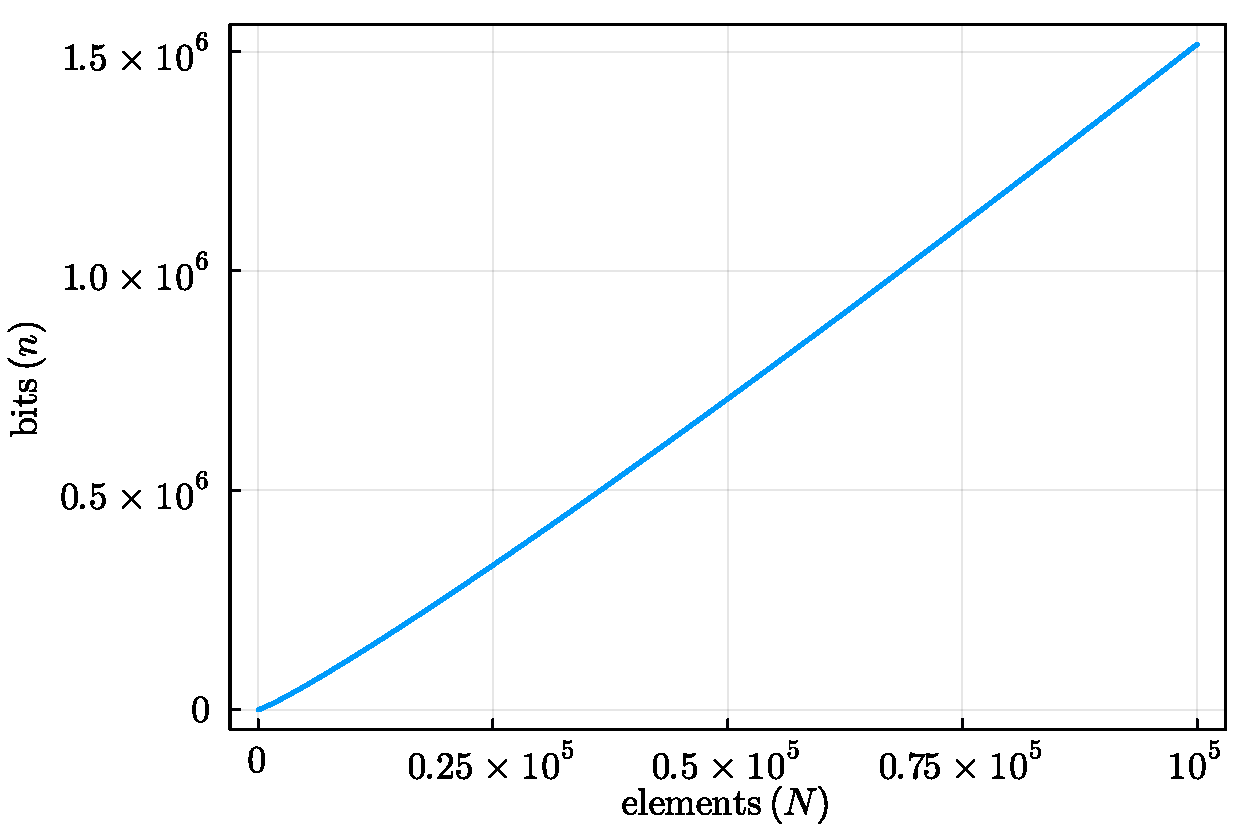
\includegraphics[width=\columnwidth]{figures/bits_permutations.pdf}
%	\caption{\textbf{Number of bits required to encode an arbitrary node permutation.} This upper-bounds the required $n$ for the consensus group.} \label{fig:bits_permutations}	
%\end{figure}

\section{Consensus assignment problem} \label{sec:consensus_assignment_problem}

The random subset problem randomly partitions network space into consensus sets, imposing a subset-sum constraint on consensus set sizes. In the context of symmetric load where all nodes request $|\mathcal{C}|$ consensus load the net consensus load is,
\begin{align}
	L = |\mathcal{C}| \cdot |\mathcal{N}|.
\end{align}
This requires performing $|\mathcal{C}|$ independent re-partitionings within each of which every node will be assigned exactly once. Under this allocation every node both contributes and requests $|\mathcal{C}|$ units of work.

The \emph{consensus assignment problem} generalises the random subset problem to accommodate arbitrary consensus set sizes and asymmetric load, allowing nodes to contribute and request arbitrary consensus workload, a prerequisite for enabling a free consensus market.

Representing consensus assignment via \emph{consensus assignment graphs} (Sec.~\ref{sec:assign_graphs}) reflecting the contributed and requested load by nodes and consensus sets, the algorithm uniformly samples from the space of satisfying assignments (Sec.~\ref{sec:uniform_consensus_samp}), achieved by defining consensus assignment via its algebraic group structure (Sec.~\ref{sec:assign_group}) and uniformly sampling the group action acting on an initial graph assignment (Sec.~\ref{sec:initial_graph_assignment}), where the pseudo-random algorithm is seeded (Sec.~\ref{sec:random_bitstreams}) by a secure random variable established by the network (Sec.~\ref{sec:secure_shared_randomness}) to ensure consistent evaluation in a distributed context. The distributed algorithm for the consensus assignment problem is shown in Alg.~\ref{alg:uniform_consensus_sampling}.

\begin{algorithm}[H]
\begin{algorithmic}
\Function{DistConsensusSampling}{$\mathcal{N}$, $U$, $V$, $d$} $\to E$ 
	\State $\mathcal{X}_\mathcal{N} \gets \textsc{SecureSharedRandomness}(\mathcal{N})$
	\State $E \gets \textsc{CanonicalGraph}(U,V,d)$
	\State $E \gets \textsc{ConsensusShuffle}(\mathcal{X}_\mathcal{N}, E)$
	\State \Return $E$
\EndFunction
\end{algorithmic}	
\caption{Distributed algorithm for the consensus assignment problem. A secure shared random variable (Sec.~\ref{sec:secure_shared_randomness}), $\mathcal{X}_\mathcal{N}$, collectively established by the network, $\mathcal{N}$, seeds pseudo-random sampling (Sec.~\ref{sec:uniform_consensus_samp}) over consensus assignments, $E$, satisfying the consensus assignment graph constraints, $(U,V,d)$ (Sec.~\ref{sec:assign_graphs}).} \label{alg:uniform_consensus_sampling}
\end{algorithm}

\subsection{Consensus assignment graphs} \label{sec:assign_graphs}

\begin{figure}[!htb]
	\centering
	\begin{tikzpicture}[genericStyle, every node/.style={circle, draw, minimum size=2em}]
    \def\UVsep{2.8}

    \foreach \i in {1,...,5} {
            \node[draw=none] (a\i) at (0,-\i) {};
        }
    \foreach \i in {1,...,5} {
            \node[draw=none] (b\i) at (\UVsep,-\i) {};
        }

    \node[nodeNetworkStyle, rectangle, rounded corners=5pt, fit=(a1) (a5), inner sep=4pt] (rectU) {};
    \node[nodeConsensusStyle, rectangle, rounded corners=5pt, fit=(b1) (b5), inner sep=4pt] (rectV) {};

    \node[draw=none, above=-0.2em of rectU] (labelU) {$U$};
    \node[draw=none, above=-0.2em of rectV] (labelV) {$V$};
    \node[draw=none] at ($(labelU)!0.5!(labelV)$) {$E$};

    \node[nodeGrayStyle] (a1) at (0,-1) {};
    \node[nodeGrayStyle] (a2) at (0,-2) {$u_i$};
    \node[nodeGrayStyle] (a3) at (0,-3) {};
    \node[draw=none] (a4) at (0,-4) {\LARGE $\vdots$};
    \node[nodeGrayStyle] (a5) at (0,-5) {};

    \node[nodeGrayStyle] (b1) at (\UVsep,-1) {};
    \node[nodeGrayStyle] (b2) at (\UVsep,-2) {};
    \node[nodeGrayStyle] (b3) at (\UVsep,-3) {$v_j$};
    \node[draw=none] (b4) at (\UVsep,-4) {\LARGE $\vdots$};
    \node[nodeGrayStyle] (b5) at (\UVsep,-5) {};

    \foreach \i in {1,...,5} {
            \foreach \j in {1,...,5} {
                    \draw[graphNonEdgeStyle] ($(rectU.east |- a\i) + (0.01,0)$) -- ($(rectV.west |- b\j) + (-0.01,0)$);
                }
        }

    \draw[->, black, line width=0.8, line cap=round] (rectU.east |- a2) -- node[draw=none, draw=none, text=black, above=-1em,midway] {$e=(u_i,v_j)$} (rectV.west |- b3);
\end{tikzpicture}
	%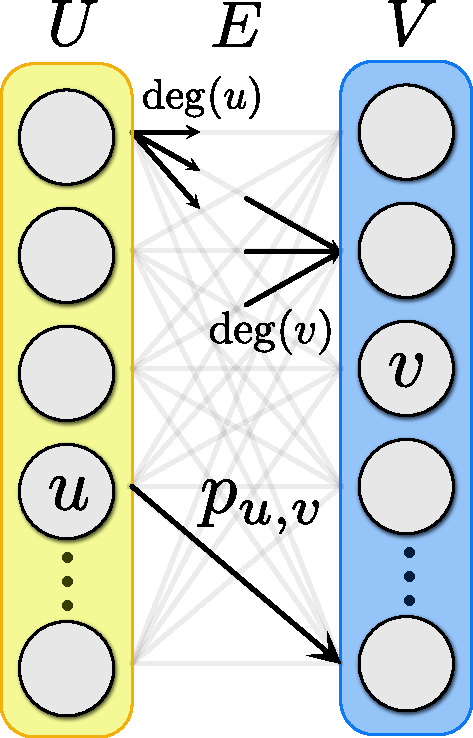
\includegraphics[width=0.4\columnwidth]{figures/bipartite_map.pdf}
	\caption{\textbf{Generalised consensus assignment problem.} Consensus assignment may be represented as a directed bipartite graph, \mbox{$\mathcal{G}=(U,V,E)$}, from a space of network nodes, $U\equiv\mathcal{N}$, to consensus sets, $V\equiv\{\mathcal{C}\}$, where vertex degree represents contributed/consumed consensus load. The set of all satisfying edge-sets $\{E\}$ represents the space of valid assignments. Under sampling, $p_{i,j}$ is the probability of the existence of edge \mbox{$e=(u_i,v_j)$}, which assigns node $u_i$ to consensus set $v_j$.}\label{fig:bipartite_map}
\end{figure}

\begin{figure}[!htb]
	\centering
	\resizebox{0.32\columnwidth}{!}{
    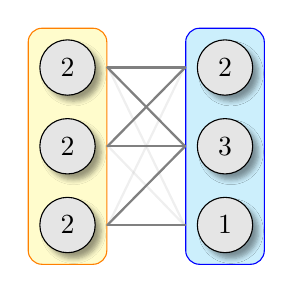
\begin{tikzpicture}[every node/.style={circle,draw,minimum size=2em}, >=latex,
            myshadow/.style={
                    blur shadow={shadow blur steps=5}
                }
        ]
        \def\UVsep{2}
        \definecolor{verylightgray}{rgb}{0.9, 0.9, 0.9}
        \colorlet{verylightblue}{cyan!20}
        \colorlet{verylightorange}{orange!20}

        \foreach \i in {1,...,3} {
                \node[draw=none] (a\i) at (0,-\i) {};
            }
        \foreach \i in {1,...,3} {
                \node[draw=none] (b\i) at (\UVsep,-\i) {};
            }

        \node[draw=orange, rectangle, rounded corners=5pt, fit=(a1) (a3), inner sep=4pt, fill=yellow, fill opacity=0.2] (rectU) {};
        \node[draw=blue, rectangle, rounded corners=5pt, fit=(b1) (b3), inner sep=4pt, fill=verylightblue] (rectV) {};

        % \node[draw=none,above=-1.2em of rectU] (labelU) {\small $\mathrm{deg}(U)$};
        % \node[draw=none,above=-1.2em of rectV] (labelV) {\small $\mathrm{deg}(V)$};
        % \node[draw=none] at ($(labelU)!0.5!(labelV)$) {\small $|E|=6$};

        \node[fill=verylightgray,myshadow] (a1) at (0,-1) {$2$};
        \node[fill=verylightgray,myshadow] (a2) at (0,-2) {$2$};
        \node[fill=verylightgray,myshadow] (a3) at (0,-3) {$2$};

        \node[fill=verylightgray,myshadow] (b1) at (\UVsep,-1) {$2$};
        \node[fill=verylightgray,myshadow] (b2) at (\UVsep,-2) {$3$};
        \node[fill=verylightgray,myshadow] (b3) at (\UVsep,-3) {$1$};

        \foreach \i in {1,...,3} {
                \foreach \j in {1,...,3} {
                        \draw[-,lightgray, opacity=0.25,line width=0.8,line cap=round] ($(rectU.east |- a\i) + (0.01,0)$) -- ($(rectV.west |- b\j) + (-0.01,0)$);
                    }
            }

        \draw[-,gray,line width=0.8,line cap=round] (rectU.east |- a1) -- (rectV.west |- b1);
        \draw[-,gray,line width=0.8,line cap=round] (rectU.east |- a1) -- (rectV.west |- b2);

        \draw[-,gray,line width=0.8,line cap=round] (rectU.east |- a2) -- (rectV.west |- b1);
        \draw[-,gray,line width=0.8,line cap=round] (rectU.east |- a2) -- (rectV.west |- b2);

        \draw[-,gray,line width=0.8,line cap=round] (rectU.east |- a3) -- (rectV.west |- b2);
        \draw[-,gray,line width=0.8,line cap=round] (rectU.east |- a3) -- (rectV.west |- b3);
    \end{tikzpicture}
}
\hfill
\resizebox{0.32\columnwidth}{!}{
    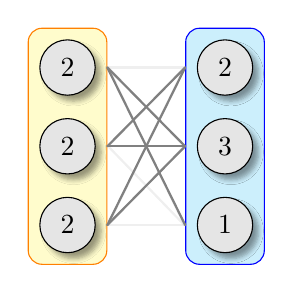
\begin{tikzpicture}[every node/.style={circle,draw,minimum size=2em}, >=latex,
            myshadow/.style={
                    blur shadow={shadow blur steps=5}
                }
        ]
        \def\UVsep{2}
        \definecolor{verylightgray}{rgb}{0.9, 0.9, 0.9}
        \colorlet{verylightblue}{cyan!20}
        \colorlet{verylightorange}{orange!20}

        \foreach \i in {1,...,3} {
                \node[draw=none] (a\i) at (0,-\i) {};
            }
        \foreach \i in {1,...,3} {
                \node[draw=none] (b\i) at (\UVsep,-\i) {};
            }

        \node[draw=orange, rectangle, rounded corners=5pt, fit=(a1) (a3), inner sep=4pt, fill=yellow, fill opacity=0.2] (rectU) {};
        \node[draw=blue, rectangle, rounded corners=5pt, fit=(b1) (b3), inner sep=4pt, fill=verylightblue] (rectV) {};

        % \node[draw=none,above=-1.2em of rectU] (labelU) {\small $\mathrm{deg}(U)$};
        % \node[draw=none,above=-1.2em of rectV] (labelV) {\small $\mathrm{deg}(V)$};
        % \node[draw=none] at ($(labelU)!0.5!(labelV)$) {\small $|E|=6$};

        \node[fill=verylightgray,myshadow] (a1) at (0,-1) {$2$};
        \node[fill=verylightgray,myshadow] (a2) at (0,-2) {$2$};
        \node[fill=verylightgray,myshadow] (a3) at (0,-3) {$2$};

        \node[fill=verylightgray,myshadow] (b1) at (\UVsep,-1) {$2$};
        \node[fill=verylightgray,myshadow] (b2) at (\UVsep,-2) {$3$};
        \node[fill=verylightgray,myshadow] (b3) at (\UVsep,-3) {$1$};

        \foreach \i in {1,...,3} {
                \foreach \j in {1,...,3} {
                        \draw[-,lightgray, opacity=0.25,line width=0.8,line cap=round] ($(rectU.east |- a\i) + (0.01,0)$) -- ($(rectV.west |- b\j) + (-0.01,0)$);
                    }
            }

        \draw[-,gray,line width=0.8,line cap=round] (rectU.east |- a1) -- (rectV.west |- b3);
        \draw[-,gray,line width=0.8,line cap=round] (rectU.east |- a1) -- (rectV.west |- b2);

        \draw[-,gray,line width=0.8,line cap=round] (rectU.east |- a2) -- (rectV.west |- b1);
        \draw[-,gray,line width=0.8,line cap=round] (rectU.east |- a2) -- (rectV.west |- b2);

        \draw[-,gray,line width=0.8,line cap=round] (rectU.east |- a3) -- (rectV.west |- b2);
        \draw[-,gray,line width=0.8,line cap=round] (rectU.east |- a3) -- (rectV.west |- b1);
    \end{tikzpicture}
}
\hfill
\resizebox{0.32\columnwidth}{!}{
    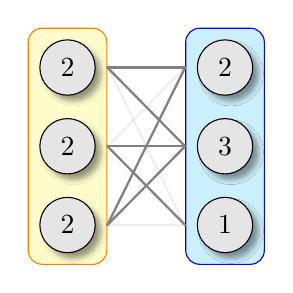
\begin{tikzpicture}[every node/.style={circle,draw,minimum size=2em}, >=latex,
            myshadow/.style={
                    blur shadow={shadow blur steps=5}
                }
        ]
        \def\UVsep{2}
        \definecolor{verylightgray}{rgb}{0.9, 0.9, 0.9}
        \colorlet{verylightblue}{cyan!20}
        \colorlet{verylightorange}{orange!20}

        \foreach \i in {1,...,3} {
                \node[draw=none] (a\i) at (0,-\i) {};
            }
        \foreach \i in {1,...,3} {
                \node[draw=none] (b\i) at (\UVsep,-\i) {};
            }

        \node[draw=orange, rectangle, rounded corners=5pt, fit=(a1) (a3), inner sep=4pt, fill=yellow, fill opacity=0.2] (rectU) {};
        \node[draw=blue, rectangle, rounded corners=5pt, fit=(b1) (b3), inner sep=4pt, fill=verylightblue] (rectV) {};

        % \node[draw=none,above=-1.2em of rectU] (labelU) {\small $\mathrm{deg}(U)$};
        % \node[draw=none,above=-1.2em of rectV] (labelV) {\small $\mathrm{deg}(V)$};
        % \node[draw=none] at ($(labelU)!0.5!(labelV)$) {\small $|E|=6$};

        \node[fill=verylightgray,myshadow] (a1) at (0,-1) {$2$};
        \node[fill=verylightgray,myshadow] (a2) at (0,-2) {$2$};
        \node[fill=verylightgray,myshadow] (a3) at (0,-3) {$2$};

        \node[fill=verylightgray,myshadow] (b1) at (\UVsep,-1) {$2$};
        \node[fill=verylightgray,myshadow] (b2) at (\UVsep,-2) {$3$};
        \node[fill=verylightgray,myshadow] (b3) at (\UVsep,-3) {$1$};

        \foreach \i in {1,...,3} {
                \foreach \j in {1,...,3} {
                        \draw[-,lightgray, opacity=0.25,line width=0.8,line cap=round] ($(rectU.east |- a\i) + (0.01,0)$) -- ($(rectV.west |- b\j) + (-0.01,0)$);
                    }
            }

        \draw[-,gray,line width=0.8,line cap=round] (rectU.east |- a1) -- (rectV.west |- b1);
        \draw[-,gray,line width=0.8,line cap=round] (rectU.east |- a1) -- (rectV.west |- b2);

        \draw[-,gray,line width=0.8,line cap=round] (rectU.east |- a2) -- (rectV.west |- b2);
        \draw[-,gray,line width=0.8,line cap=round] (rectU.east |- a2) -- (rectV.west |- b3);

        \draw[-,gray,line width=0.8,line cap=round] (rectU.east |- a3) -- (rectV.west |- b2);
        \draw[-,gray,line width=0.8,line cap=round] (rectU.east |- a3) -- (rectV.west |- b1);
    \end{tikzpicture}
}
	\caption{\textbf{Satisfying solutions for the consensus assignment problem.}. The space of satisfying edge-sets, $E$, for degree sequence \mbox{$d=(2,2,2;2,3,1)$}, \mbox{$|E|=6$} edges, and \mbox{$|C(d)|=3$} graph realisations. Nodes are labelled by vertex degree.}\label{fig:edge_assignments}
\end{figure}

Consider a directed bipartite graph (Fig.~\ref{fig:bipartite_map}),
\begin{align}
	\mathcal{G} = (U,V,E),
\end{align}
where vertices $u\in U$ and $v\in V$ represent network nodes (\mbox{$U=\mathcal{N}$}) and consensus sets (\mbox{$V=\mathcal{\{\mathcal{C}\}}$}) respectively, and the directed edge set $E$ defines the assignment of nodes to consensus sets where each edge is associated with a unit of consensus work. The constraint that nodes may be assigned at most once to a given consensus set imposes that $G$ is a simple graph.

Consensus load may be arbitrarily partitioned and nodes may make multiple requests for consensus sets, hence in general $|\mathcal{S}|\neq|\{\mathcal{C}\}|$. %Expressing vertex sets as degree sequences,
%\begin{align}
%	U &= (\mathrm{deg}(u_1),\dots,\mathrm{deg}(u_{|U|})), \nonumber\\
%	V &= (\mathrm{deg}(v_1),\dots,\mathrm{deg}v_{|V|})),
%\end{align}

Vertex degrees represent workload, where $\mathrm{deg}(u)$ denotes work contributed by node $u$ and $\mathrm{deg}(v)$ the load requested by consensus set $v$. The degree sum formula for bipartite graphs equates to a conservation of work constraint in the system,
\begin{align} \label{eq:degree_sum}
	\sum_{u\in U} \mathrm{deg}(u) = \sum_{v\in V} \mathrm{deg}(v) = |E|,
\end{align}
where $|E|$ represents net consensus work.

Asymmetric load introduces sampling bias into the average-case likelihood of compromise, $r$, defined in Eq.~\eqref{eq:av_r_uniform}, which generalises to,
\begin{align}
	r = \frac{1}{|E|} \sum_{i=1}^{|\mathcal{N}|} \mathrm{deg}(u_i) \cdot r_i.
\end{align}

The assignment of network nodes to consensus sets is equivalent to assigning edge-sets $E$ subject to the constraints imposed by the degree sequence,
\begin{align} \label{eq:degree_seq}
	d = (&\mathrm{deg}(u_1),\dots,\mathrm{deg}(u_{|U|});\nonumber\\
	&\mathrm{deg}(v_1),\dots,\mathrm{deg}(v_{|V|})),
\end{align}
where,
\begin{align}
	|d| = |U|+|V| = |\mathcal{N}|+|\{\mathcal{C}\}|.
\end{align}
Expressing graphs by their edge-sets, $E$,
\begin{align}
	\mathcal{G} = \{(u_e\in U, v_e\in V)\}_{e\in E},
\end{align}
where edges $(u_e,v_e)$ denote the assignment of node $u_e$ to consensus set $v_e$. In columnar representation,
\begin{align}
	E_U &= \{u_e\}_{e\in E},\nonumber\\
	E_V &= \{v_e\}_{e\in E},	
\end{align}
elements have multiplicity given by their degree.

\subsection{Consensus group} \label{sec:assign_group}

\begin{figure}[!htb]
	\centering
	\begin{tikzpicture}[genericStyle, every node/.style={circle, draw, minimum size=1.7em, text width=1em, align=center, inner sep=0pt}]
    \def\UVsep{2.5em}
    \def\colSep{3em}
    \def\rowSep{1.2em}
    \def\hStep{0.7em}

    % Figure 1
    \node[nodeUStyle] (a1) at (0,0) {$u_i$};
    \node[nodeUStyle] (a2) [below=\hStep of a1] {$u_j$};
    \node[nodeVStyle, right=\UVsep of a1] (b1) {$v_i$};
    \node[nodeVStyle, right=\UVsep of a2] (b2) {$v_j$};

    \draw[graphEdgeStyle] (a1) -- (b1); 
    \draw[graphEdgeStyle] (a2) -- (b2);

    \coordinate (midA) at ($(a1.south)!0.5!(a2.north)$);
    \node[draw=none, left=0.4em of midA]
    {$\Big\updownarrow$};

    \node[nodeUStyle, right=\colSep of b1] (c1) {$u_i$};
    \node[nodeUStyle, right=\colSep of b2] (c2) {$u_j$};
    \node[nodeVStyle, right=\UVsep of c1] (d1) {$v_i$};
    \node[nodeVStyle, right=\UVsep of c2] (d2) {$v_j$};

    \draw[graphEdgeStyle] (c1) -- (d2); 
    \draw[graphEdgeStyle] (c2) -- (d1);

    \coordinate (midB) at ($(b1.east)!0.5!(b2.east)$); 
    \coordinate (midC) at ($(c1.west)!0.5!(c2.west)$);
    \coordinate (midBC) at ($(midB)!0.5!(midC)$);
    \node[draw=none, text width=2em] at (midBC) {$\Longleftrightarrow$};  

    % Figure 2
    \node[nodeUStyle] (a3) [below=\rowSep of a2] {};
    \node[nodeUStyle] (a4) [below=\hStep of a3] {};

    \coordinate (midA2) at ($(a3.south)!0.5!(a4.north)$);
    \node[draw=none, left=0.4em of midA2]
    {$\Big\updownarrow$};

    \coordinate (midA3) at ($(a3.east)!0.5!(a4.east)$);
    \node[nodeVStyle, right=\UVsep of midA3] (b3) {};
    \draw[graphEdgeStyle] (a3) -- (b3);
    \draw[graphEdgeStyle] (a4) -- (b3);

    \node[nodeUStyle, below=\rowSep of c2] (c3) {};
    \node[nodeUStyle, below=\hStep of c3] (c4) {};

    \coordinate (midC3) at ($(c3.east)!0.5!(c4.east)$);
    \node[nodeVStyle, right=\UVsep of midC3] (d3) {};
    \draw[graphEdgeStyle] (c3) -- (d3);
    \draw[graphEdgeStyle] (c4) -- (d3);

    \coordinate (midC2) at ($(c3.west)!0.5!(c4.west)$);
    \coordinate (midBC2) at ($(b3.east)!0.5!(midC2)$);
    \node[draw=none, text width=2em] at (midBC2) {$\Longleftrightarrow$};  
\end{tikzpicture}

	%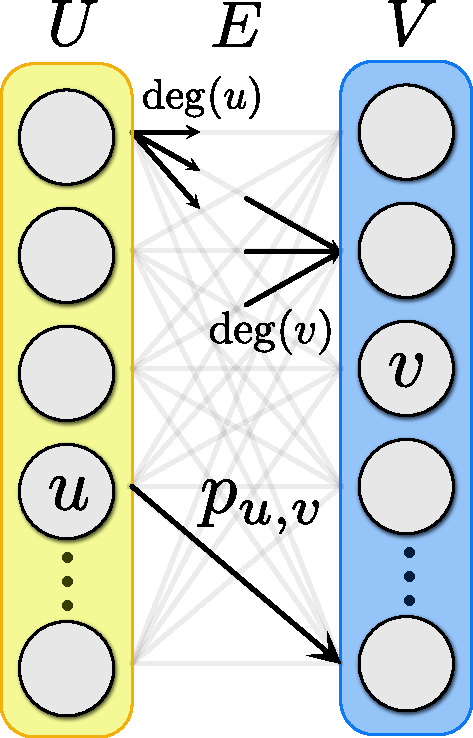
\includegraphics[width=0.4\columnwidth]{figures/bipartite_map.pdf}
	\caption{\textbf{Swap symmetry.}???.}\label{fig:swap_symmetry}
\end{figure}

* Clarify edge transformations rather than U and V.

* Permutation group

* Graph automorphisms not the same as automorphisms over edges.

* Automorphism group in edge space describes invariances. Sym/Aut gives consensus group?

* Automorphism group over edge permutations is in general inequivalent to the conventional definition of a graph automorphism: for $\mathcal{G}=(V,E)$, $(u,v)\in E \Leftrightarrow (\sigma(u),\sigma(v))\in E$ %$\mathrm{Aut}(\mathcal{G}): $

* Counting graph automorphisms is known to be 

* While all permutations within $E_U$ and $E_V$ are degree preserving, not all are unique.

Transformations over the space of satisfying graph realisations of given degree sequence, $d$, defines the \emph{consensus group}, $C(d)$, fully characterised by its degree sequence. Over the space of satisfying graphs the consensus group,
\begin{align}
	\phi: C(d)\times \mathcal{G}_d \to \mathcal{G}_d,
\end{align}
is identically the symmetric group,
\begin{align}
	\phi: C(d) = \mathrm{Sym}(\mathcal{G}_d).
\end{align}
The action of the consensus group may be equivalently defined via permutations within the columns of satisfying edge-sets,
\begin{align}
	\psi: C(d)\times (E_U\times E_V) \to (E_U\times E_V),
\end{align}
the group of non-degenerate permutations within the columns of $E$, which discounts permutations under which edge-sets remain invariant, a subgroup of the symmetric group acting on either column, both of length $|E|$,
\begin{align}
	(\psi, E_{U,V}) &\subseteq S_{|E|}.
\end{align}

In the special case of 1-regular graphs, satisfying consensus assignments define bijective maps across graph partitions and the group action over edge-set columns is identically the symmetric group,
\begin{align}
	\psi: C(d) = S_{|E|},\,\delta(\mathcal{G})=\Delta(\mathcal{G})=1,
\end{align}
as there are no degenerate permutations.

Hence, the order of the consensus group, equivalently the number of unique consensus assignments, is upper-bounded by the order of the symmetric group acting on edge-sets, $S_{|E|}$,
\begin{align} \label{eq:orbit_order}
	%|C(d)| &= \frac{|E|!}{\prod_{u\in U}\mathrm{deg}(u)!\cdot \prod_{v\in V}\mathrm{deg}(v)!} \nonumber\\
	%&= \binom{|E|!}{d_1,\dots,d_{|U|+|V|}} \nonumber\\
	|C(d)| &\leq |E|!,
\end{align}
with equality when \mbox{$\Delta(\mathcal{G})=1$}.

Employing element-wise inequality notation for degree sequences, of equal length, \mbox{$|d|=|d'|$},
\begin{align}
	d' < d \coloneqq d'_i < d_i,\, \forall\, i,
\end{align}
affords the equivalent relations between degree sequences, satisfying assignment graphs and their respective subgroup structures,
\begin{align} \label{eq:sub_dgc}
	d' < d &\Rightarrow \mathcal{G}_{d'} \subset \mathcal{G}_d \Rightarrow C(d') \triangleleft C(d),
\end{align}
where $C(d')$ is a normal subgroup of $C(d)$ and $\mathcal{G}_{d'}$ is a subgraph of $\mathcal{G}_d$ under edge-removal.

%Consensus groups exhibit a recursive normal subgroup structure,
%\begin{align}
%	C(d') &\triangleleft C(d),
%\end{align}
%reflecting the associated subgraph structure,
%\begin{align}
%	\mathcal{G}' &\subset \mathcal{G}.
%\end{align}

%As edge exchange operations are symmetric across $U$ and $V$ the consensus group may equivalently be associated with the space of edge permutations on either. Despite having support over vertex sets with distinct degree sequences they afford the same space of edge permutations.

The number of bits required to uniquely address the group's orbit scales as (Fig.~\ref{fig:bits_permutations}),
\begin{align}
	n &= \log_2(|\mathrm{Orb}_C(E)|) \leq \log_2(|E|!).
\end{align}

\begin{figure}[!htb]
	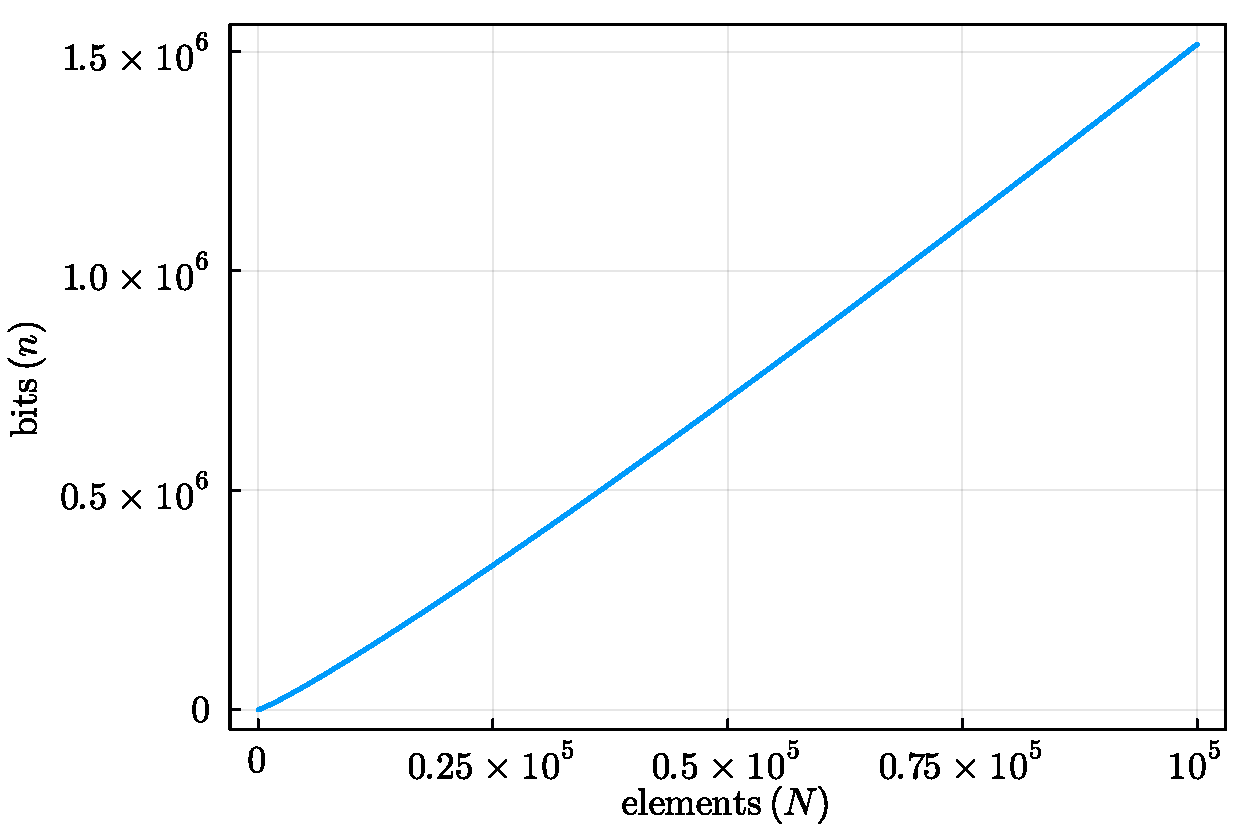
\includegraphics[width=\columnwidth]{figures/bits_permutations.pdf}
	\caption{\textbf{Number of bits ($n$) required to encode an arbitrary permutation ($S_N$) over $N$ elements.} This upper-bounds the required number of bits to uniquely address elements of the consensus group, $C(d)$.} \label{fig:bits_permutations}
\end{figure}

\subsection{Uniform consensus sampling} \label{sec:uniform_consensus_samp}

Secure consensus assignment requires assigning edge-sets uniformly at random over the space of all satisfying edge-sets. Uniformity implies maximisation of entropy, given by,
\begin{align}
	H(C(d)) = \log_2(|C(d)|),
\end{align}
where $|C(d)|$ is the order of the respective consensus group. Degeneracies in permutations result in sampling bias thereby reducing entropy, requiring that algorithmic implementation does not double-count degenerate permutations from the symmetric group.

\subsubsection{Fisher-Yates shuffle}

The Fisher-Yates shuffle \cite{FisherYates53} is an efficient algorithm for applying in-place permutations $\pi\in S_n$ to an array of $n$ elements uniformly at random (Alg.~\ref{alg:fisher_yates}).

The algorithm iteratively allows every array index to randomly exchange itself with any element not already assigned. Assuming $O(1)$ random number generation the Fisher-Yates shuffle exhibits $O(n)$ time-complexity. As the operational primitive is the exchange operation the algorithm permutes arrays in-place.

The sequence of $O(n)$ random numbers chosen during execution defines a decision tree whose $i$th level assigns the $i$th array index. Individual execution paths correspond to individual permutations with a one-to-one correspondence. Hence, the algorithm's execution space $\mathcal{L}_n$ is isomorphic to the symmetric group,
\begin{align}
	\mathcal{L}_n \cong S_n,
\end{align}
under mapping between execution paths \mbox{$l\in\mathcal{L}_n$} and permutations \mbox{$\pi\in S_n$}. As all execution paths occur with uniform probability $1/n!$ the algorithm uniformly samples from the symmetric group.

\begin{algorithm}[H]
\begin{algorithmic}
\Function{FisherYatesShuffle}{$\vec{v}$} $\to \vec{v}$ \Comment{$O(n)$}
	\For{$i \gets |\vec{v}|-1 \textbf{ to } 1$} \Comment{$O(n)$}
		\State $j \gets \textsc{Random}(\{0,\dots,i\})$ \Comment{$O(1)$}
		\State $v_i\leftrightarrow v_j$ \Comment{Exchange}
	\EndFor
	\State \Return $\vec{v}$
\EndFunction
\end{algorithmic}	
\caption{\cite{FisherYates53} The Fisher-Yates shuffle algorithm for applying a random permutation $\pi\in S_{|\vec{v}|}$ to the elements a vector $\vec{v}$. The algorithm permutes  vectors in-place with $O(n)$ runtime assuming an $O(1)$ \textsc{Random}($\cdot$) function.}\label{alg:fisher_yates}
\end{algorithm}

The uniqueness of execution paths may be seen by noting that an element at index $j\leq i$ has  exactly one path to be reassigned to index $i$, via the direct exchange $v_i\leftrightarrow v_j$ when the loop reaches index $i$.

The execution path $l\in\mathcal{L}_n$ of the algorithm directly relates to the cycle decomposition of the respective group element. As the algorithm iterates through $i$ the series of exchange operations defines a path. When a trivial $v_i\leftrightarrow v_i$ exchange occurs it terminates that path, closing it as a cycle, after which the next $i$ opens a new one.

Closely related to the Fisher-Yates shuffle is Sattolo's algorithm \cite{Sattolo86} for uniformly sampling the cyclic group ($C_n$) differing only from the Fisher-Yates shuffle in the set of allowed exchanges,
\begin{align}
	\text{Fisher-Yates }(S_n):\,\,& 0\leq j\leq i,\nonumber\\
	\text{Sattolo }(C_n):\,\,& 0\leq j<i.
\end{align}
Note that this distinction serves to prohibit trivial exchanges ($v_i\leftrightarrow v_i$) thereby forcing all execution paths to define single cycles.

\subsubsection{Generalised Fisher-Yates shuffle for finite groups}

The Fisher-Yates shuffle may be generalised to uniformly sample over other finite groups (Alg.~\ref{alg:fisher_yates_general}).

Alg.~\ref{alg:fisher_yates} may be interpreted as follows: for every index $i$ the associated value $v_i$ is chosen uniformly from the set of unassigned values $v_j$ (where $0\leq j\leq i$). More generally, we would choose $v_i$ uniformly from the set of elements it is allowed to transition to under the action of the respective group. For the symmetric group, $S_n$, this includes all elements, whereas other groups in general constrain the set of allowed transitions.

Consider a group $G$ defined over set $X$,
\begin{align}
	\phi: G\times X \to X.	
\end{align}
Elements of the set $x\in X$ individually transform under the group action of $G$ to their orbit,
\begin{align}
	\mathrm{Orb}_G(x) &= G\times x \nonumber\\
	&= \{ y\in X \,\,|\,\, \exists \,g\in G \,\,|\,\, y=g\cdot x\}
\end{align}
defining sets for the allowed transitions of $x$ under the action of $G$. For the symmetric group we have,
\begin{align}
	\mathrm{Orb}_{S_n}(x) = X,
\end{align}
as all elements may map to all others, while for other groups the orbit of $x$ may be a subset of elements.

We define the \emph{transition set}, $t$, to be the set of allowed transitions of $x$ under the group action of $G$, given by the intersection unassigned elements ($s$) and the orbit of $x$,
\begin{align}
	t = \mathrm{Orb}_G(x) \cap s.
\end{align}

%Sattolo's algorithm for uniformly sampling the cyclic group defines the transition set to include all unassigned elements excluding element $i$. This arises because under a cyclic permutation all elements must permute

\begin{algorithm}[H]
\begin{algorithmic}
\Function{GroupShuffle}{$\vec{v}$, $G$} $\to \vec{v}$\Comment{$O(n^2)$}
	\For{$i \gets |\vec{v}|-1 \textbf{ to } 1$} \Comment{$O(n)$}
		\State $s \gets \{\vec{v}_j\,|\, 0\leq j\leq i\}$ \Comment{Unassigned elements}
		\State $t \gets \textsc{TransitionSet}(\vec{v}_i,s,G)$ \Comment{$O(n)$}
		\State $j \gets \textsc{Random}(t)$ \Comment{$O(1)$}
		\State $v_i\leftrightarrow v_j$ \Comment{Exchange}
	\EndFor
	\State \Return $\vec{v}$
\EndFunction
\\
\Function{TransitionSet}{$x$, $s$, $G$} $\to t$ \Comment{$O(n)$}
	\State \Return $(G\times x) \cap s$ \Comment{Group action on reduced set}
\EndFunction
\end{algorithmic}	
\caption{Generalised Fisher-Yates shuffle for finite groups $G$.}\label{alg:fisher_yates_general}
\end{algorithm}

\textbf{WRONG FOR THE CONSENSUS GROUP:} The uniqueness of execution paths in the generalised algorithm follows the same argument as for the the original scheme. The probability associated with an execution path is,
\begin{align} \label{eq:group_order_shuffle}
	P(\vec{d}) &= \prod_{i=1}^{n} p(\vec{d}_i) = \prod_{i=1}^{n} \frac{1}{|t_i|} = \prod_{i=1}^{n} \frac{1}{|\mathrm{Orb}_{G^{(i)}}(x_i)|},
\end{align}
where \mbox{$\vec{d}_i=1/|t_i|$} is the probability of making choice \mbox{$j=\vec{d}_i$} at level $i$ under uniform sampling, and $G^{(i)}$ denotes the $i$th level subgroup of $G=G^{(n)}$ acting on the reduced set predicated on the removal of already assigned elements of $X$,
\begin{align} \label{eq:subgroup_struct}
	G^{(i)} &\times X^{(i)} \to X^{(i)},\nonumber\\
	X^{(i)} &= X\backslash\{x_{k}\}_{k>i},\nonumber\\
	G^{(i-1)} &\triangleleft G^{(i)},
\end{align}
defining a composition series followed by the algorithm to iteratively assign set elements,
\begin{align}
	1 = G^{(0)} \triangleleft \cdots \triangleleft G^{(n-1)} \triangleleft G^{(n)} = G,
\end{align}
where each subgroup acts on the set predicated on the removal of an element from the set upon which the supergroup acts.

As the consensus group is both free\footnote{Free groups: all elements are invariant under the action of all group elements except the identity,
\begin{align}
	g\cdot x = x\, \Rightarrow\, g=e.\nonumber
\end{align}} and transitive\footnote{Transitive groups: all elements $x\in X$ map to all elements $y\in X$ under the action of some group element $g\in G$,
\begin{align}
	x,y\in X \,|\, \exists\, g\in G \,\,|\,\, g\cdot x=y.\nonumber
\end{align}}
it has regular\footnote{Regular group action: $\forall\,\,x,y\in X \,\,|\,\, g\cdot x=y$, $g\in G$ is unique.} group action and all group elements have the same orbit. Hence, $|t_i|$ is level-dependent on $i$ but independent of group element $x\in X$ and execution pathway $l\in\mathcal{L}$. $P(\vec{d})$ is therefore a function of the group but uniform across all group elements.

\subsubsection{Uniformly sampling the consensus group}

Uniformly sampling the consensus group is achieved by defining transition sets as per Alg.~\ref{alg:consensus_shuffle}, whereby allowed transitions under edge exchanges \mbox{$v_i\leftrightarrow v_j$} satisfy the Boolean constraint,
\begin{align}
	[(u_i,v_j) \not\in E] \lor [(u_j,v_i)	\not\in E] = 1,
\end{align}
requiring that newly created edges not be previously existing ones. ??? CHECK

An \mbox{$v_i\leftrightarrow v_j$} exchange within edge-set $E$ is equivalent to eliminating existing edges,
\begin{align}
	e_i = (u_i,v_i),\,\, e_j = (u_j,v_j),
\end{align}
and replacing them with permuted edges,
\begin{align}
	e_i' = (u_i,v_j),\,\, e_j' = (u_j,v_i).
\end{align}
Thus, edge-set invariance under \mbox{$v_i\leftrightarrow v_j$} requires,
\begin{align}
	E \backslash \{e_i,e_j\} \cup \{e_i',e_j'\} = E,
\end{align}
which implies,
\begin{align}
	\{e_i',e_j'\} &\in E,\nonumber\\
	E \backslash \{e_i,e_j\} &= E \backslash \{e_i',e_j'\},\nonumber\\
	\{e_i,e_j\}&=\{e_i',e_j'\}.
\end{align}
Hence, the requirement exchanges \mbox{$v_i\leftrightarrow v_j$} not be edge-set invariant is,
\begin{align}
	\{e_i',e_j'\} &\in E,\nonumber\\
	E \backslash \{e_i,e_j\} &= E \backslash \{e_i',e_j'\},\nonumber\\
	\{e_i,e_j\}&=\{e_i',e_j'\}.
\end{align}

%\begin{align}
%	E \backslash \{e_i,e_j\} = E \backslash \{e_i',e_j'\}.
%\end{align}

%As the edge-sets of simple graphs are simple sets, 

%
%* The exchange operation $v_i\leftrightarrow v_j$ prospectively creates the new edges $(u_i,v_j)$ and $(u_j,v_i)$. If either already exist this would either: violate $\mathcal{G}$ being a simple graph; constitute a degenerate edge permutation. Hence, 

* Need to clarify notation here. $i$ here refers to index in $E$, but usually we use it for a node number.

%\begin{align} \label{eq:exchange_rule}
%		(u_i \neq u_j) \odot (v_i \neq v_j) = 1,
%\end{align}
%where $\odot$ denotes logical XNOR. This constraint is equivalent to,
%\begin{align}
%		[(u_i \neq u_j) \land (v_i \neq v_j)] \lor [(u_i = u_j) \land (v_i = v_j)] = 1,
%\end{align}
%where the first clause allows exchange operations between nodes $u_i$ and $u_j$, equivalently between consensus sets $v_i$ and $v_j$, only when distinct (Fig.~\ref{fig:swap_sym}), and the second clause is equivalent to $i=j$, ensuring inclusion of $u_i$ itself.

%\begin{figure}[!htb]
%\centering
%\begin{tikzpicture}[genericStyle, every node/.style={circle, draw, minimum size=1.7em, text width=1em, align=center, inner sep=0pt}]
    \def\UVsep{2.5em}
    \def\colSep{3em}
    \def\rowSep{1.2em}
    \def\hStep{0.7em}

    % Figure 1
    \node[nodeUStyle] (a1) at (0,0) {$u_i$};
    \node[nodeUStyle] (a2) [below=\hStep of a1] {$u_j$};
    \node[nodeVStyle, right=\UVsep of a1] (b1) {$v_i$};
    \node[nodeVStyle, right=\UVsep of a2] (b2) {$v_j$};

    \draw[graphEdgeStyle] (a1) -- (b1); 
    \draw[graphEdgeStyle] (a2) -- (b2);

    \coordinate (midA) at ($(a1.south)!0.5!(a2.north)$);
    \node[draw=none, left=0.4em of midA]
    {$\Big\updownarrow$};

    \node[nodeUStyle, right=\colSep of b1] (c1) {$u_i$};
    \node[nodeUStyle, right=\colSep of b2] (c2) {$u_j$};
    \node[nodeVStyle, right=\UVsep of c1] (d1) {$v_i$};
    \node[nodeVStyle, right=\UVsep of c2] (d2) {$v_j$};

    \draw[graphEdgeStyle] (c1) -- (d2); 
    \draw[graphEdgeStyle] (c2) -- (d1);

    \coordinate (midB) at ($(b1.east)!0.5!(b2.east)$); 
    \coordinate (midC) at ($(c1.west)!0.5!(c2.west)$);
    \coordinate (midBC) at ($(midB)!0.5!(midC)$);
    \node[draw=none, text width=2em] at (midBC) {$\Longleftrightarrow$};  

    % Figure 2
    \node[nodeUStyle] (a3) [below=\rowSep of a2] {};
    \node[nodeUStyle] (a4) [below=\hStep of a3] {};

    \coordinate (midA2) at ($(a3.south)!0.5!(a4.north)$);
    \node[draw=none, left=0.4em of midA2]
    {$\Big\updownarrow$};

    \coordinate (midA3) at ($(a3.east)!0.5!(a4.east)$);
    \node[nodeVStyle, right=\UVsep of midA3] (b3) {};
    \draw[graphEdgeStyle] (a3) -- (b3);
    \draw[graphEdgeStyle] (a4) -- (b3);

    \node[nodeUStyle, below=\rowSep of c2] (c3) {};
    \node[nodeUStyle, below=\hStep of c3] (c4) {};

    \coordinate (midC3) at ($(c3.east)!0.5!(c4.east)$);
    \node[nodeVStyle, right=\UVsep of midC3] (d3) {};
    \draw[graphEdgeStyle] (c3) -- (d3);
    \draw[graphEdgeStyle] (c4) -- (d3);

    \coordinate (midC2) at ($(c3.west)!0.5!(c4.west)$);
    \coordinate (midBC2) at ($(b3.east)!0.5!(midC2)$);
    \node[draw=none, text width=2em] at (midBC2) {$\Longleftrightarrow$};  
\end{tikzpicture}

%%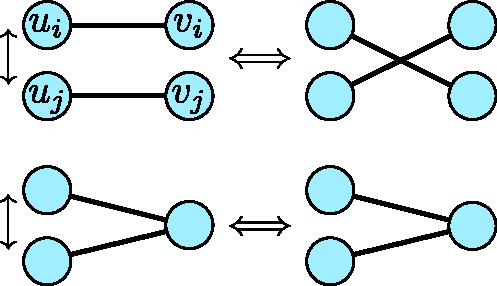
\includegraphics[width=0.5\columnwidth]{figures/swap_symmetry.pdf}
%\caption{\textbf{Degeneracy rule for vertex exchanges in the consensus group.} Allowed vertex exchanges $u_i\leftrightarrow u_j$ (equivalently $v_i\leftrightarrow v_j$) require vertices in both the $U$ and $V$ partitions of the bipartite graph to be distinct, as per Eq.~\eqref{eq:exchange_rule}.} \label{fig:swap_sym}	
%\end{figure}

\begin{algorithm}[H]
\begin{algorithmic}
\Function{ConsensusShuffle}{$\mathcal{X}$, $\vec{u}$, $\vec{v}$} $\to \vec{v}$ \Comment{$O(n^2)$}
	\For{$i \gets |\vec{v}|-1 \textbf{ to } 1$} \Comment{$O(n)$}
		\State $t \gets \{0\leq k< i \,|\, \textsc{Transition}(i,k) = 1\}$ \Comment{$O(n)$}
		\State $j \gets \textsc{Random}(\mathcal{X}, t \cup i)$ \Comment{$O(1)$}
		\State $v_i\leftrightarrow v_j$ \Comment{Exchange}
	\EndFor
	\State \Return $\vec{v}$
\EndFunction
\\
\Function{AllowTransition}{$i$, $j$} $\to \{0,1\}$ \Comment{$O(n)$}
	\State \Return $[(u_i,v_j) \notin E] \land [(u_j,v_i) \notin E]$
\EndFunction
\end{algorithmic}	
\caption{The transition set for the consensus group may be characterised by the constraints imposed by the group relations characterising non-degenerate transitions. The \textsc{Transition} function is a binary operator specifying whether index $j$ is an allowed transition for index $i$, defining the respective transition set.}\label{alg:consensus_shuffle}
\end{algorithm}

The regular action of the consensus group implies that under symmetrisation via uniform sampling all satisfying edge assignments $\{E\}$ occur with equal probability, from which it follows,
% It follows that every node $u$ will be ass, and nodes are assigned with uniform probability to all consensus sets, and every consensus set has uniform probability of comprising any subset of nodes,
\begin{align} \label{eq:prob_cons}
	p_{u,v} &= \frac{\mathrm{deg}(u)}{|V|},\nonumber\\
	\sum_{v\in V} p_{u,v} &= \mathrm{deg}(u),\nonumber\\
	\sum_{u\in U} p_{u,v} &= 1, \nonumber\\
	\sum_{u\in U, v\in V} p_{u,v} &= |E|,
\end{align}
where $p_{u,v}$ is the probability of node $u$ being assigned to consensus set $v$.
* Regular action.

* Use uniform bidding to preserve average case $r$. If non-uniform the effective $r$ in consensus sets is biased towards the $r$ of higher bidders.

* ???
* For a given edge $e=(u,v)$ in edge-set $e\in E$, the order of the orbit of vertex $v$ under the group action $\psi$ is,
\begin{align}
		\psi: |\mathrm{Orb}_C(v)| &= |V/v| = |V|-1.
\end{align}
That is, vertex $v$ may permute to any vertex other than itself.

* ??? TODO. Fig.~\ref{fig:bipartite_map}

* Bipartite decomposition or bipartite dimension. Edge-disjoint union of complete bipartite graphs or bicliques.

* Degree-preserving biclique decomposition.

* Kmn defines invariant subgraphs under edge-permutation. Vertices within a Kmn subgraph define graph automorphisms under vertex permutations $\sigma$.
\begin{align}
	\varphi: (u,v)\in E \Longleftrightarrow (\sigma_u,\sigma_v)	\in E.
\end{align}

For complete graphs all vertex permutations within each bipartition define graph automorphisms,
\begin{align}
	\mathrm{Aut}(K_{m,n}) = S_m\times S_n.
\end{align}


* Graph sum (disjoint union)
\begin{align}
\mathcal{G}_d^{(K)} = \bigoplus_{b} K_{m_b,n_b}.
\end{align}

* Not all graphs can be decomposed this way. Determining this is NP-hard in general.

For $K_{m,n}$,
\begin{align}
	\mathrm{deg}(u)&=n,\,\forall\, u\in U,\nonumber\\
	\mathrm{deg}(v)&=m,\,\forall\, v\in V.
\end{align}

* Admits graph automorphisms,
\begin{align}
	\bigtimes_{b} (S_{m_b}\times S_{n_b}) \subseteq \mathrm{Aut}(\mathcal{G}_d^{(K)}).
\end{align}
* Is it equality?

\begin{figure}[!htb]
	\begin{tikzpicture}[genericStyle]
    \def\Km{5}
    \def\Kn{4}
    \def\Kmskip{4}
    \def\Knskip{3}
    \def\voff{-0.575}
    \def\dotsoff{0.15}
    \def\UVsep{2.8}
    
    \foreach \i in {1,...,\Km} {
        \ifnum\i=\Kmskip
          \node[draw=none] (a\i) at (0,\dotsoff-\i) {\LARGE $\vdots$};
        \else
            \ifnum\i=\Km
                \node[nodeUStyle] (a\i) at (0,-\i) {$u_m$};
            \else
                \node[nodeUStyle] (a\i) at (0,-\i) {$u_{\i}$};
            \fi
        \fi
    }
    \foreach \i in {1,...,\Kn} {
        \ifnum\i=\Knskip
            \node[draw=none] (b\i) at (\UVsep,\dotsoff+\voff-\i) {\LARGE $\vdots$};
        \else
            \ifnum\i=\Kn
                \node[nodeVStyle] (b\i) at (\UVsep,\voff-\i) {$v_n$};
            \else
                \node[nodeVStyle] (b\i) at (\UVsep,\voff-\i) {$v_{\i}$};
            \fi
        \fi
    }
    
    \foreach \i in {1,...,\Km} {
        \foreach \j in {1,...,\Kn} {
        \ifnum\i=\Kmskip
        \else
            \ifnum\j=\Knskip
            \else
                \draw[graphEdgeStyle] ($(a\i.east)$) -- ($(b\j.west)$);
            \fi
        \fi
        }
    }

    \node[draw=none] at ($(a1)!0.5!(b1) + (0,0.5)$) {$K_{m,n}$};
\end{tikzpicture}
	\caption{\textbf{Complete bipartite graph, $K_{m,n}$.} Vertices in each bipartition have uniform degree.} \label{fig:K_mn_graph}
\end{figure}

\begin{figure}[!htb]
	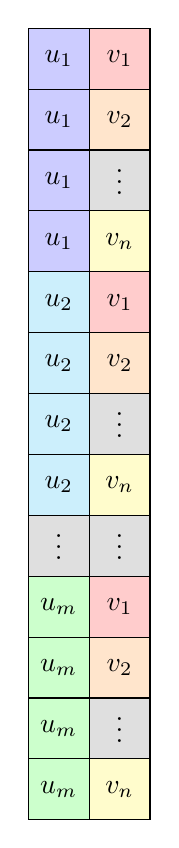
\begin{tikzpicture}
  \tikzset{square node/.style={draw, minimum size=2.2em}}

    \definecolor{verylightgray}{rgb}{0.9, 0.9, 0.9}
    \colorlet{color1}{blue!20}
    \colorlet{color2}{cyan!20}
    \colorlet{color3}{green!20}

    \colorlet{colorA}{red!20}
    \colorlet{colorB}{orange!20}
    \colorlet{colorC}{yellow!20}

  \def\x{2.2em}

    % 1
    \node[square node, fill=color1] at (\x,-\x) {$u_1$};
    \node[square node, fill=colorA] at (2*\x,-\x) {$v_1$};

    \node[square node, fill=color1] at (\x,-2*\x) {$u_1$};
    \node[square node, fill=colorB] at (2*\x,-2*\x) {$v_2$};
    
    \node[square node, fill=color1] at (\x,-3*\x) {$u_1$};
    \node[square node, fill=lightgray!50] (d1) at (2*\x,-3*\x) {};
    \node[draw=none] at (d1) [yshift=0.25em] {$\vdots$};

    \node[square node, fill=color1] at (\x,-4*\x) {$u_1$};
    \node[square node, fill=colorC] at (2*\x,-4*\x) {$v_n$};

     % 2
    \node[square node, fill=color2] at (\x,-5*\x) {$u_2$};
    \node[square node, fill=colorA] at (2*\x,-5*\x) {$v_1$};

    \node[square node, fill=color2] at (\x,-6*\x) {$u_2$};
    \node[square node, fill=colorB] at (2*\x,-6*\x) {$v_2$};
    
    \node[square node, fill=color2] at (\x,-7*\x) {$u_2$};
    \node[square node, fill=lightgray!50] (d2) at (2*\x,-7*\x) {};
    \node[draw=none] at (d2) [yshift=0.25em] {$\vdots$};

    \node[square node, fill=color2] at (\x,-8*\x) {$u_2$};
    \node[square node, fill=colorC] at (2*\x,-8*\x) {$v_n$};

    % ...
    \node[square node, fill=lightgray!50] (d3) at (\x,-9*\x) {};
    \node[draw=none] at (d3) [yshift=0.25em] {$\vdots$};
    \node[square node, fill=lightgray!50] (d4) at (2*\x,-9*\x) {};
    \node[draw=none] at (d4) [yshift=0.25em] {$\vdots$};

    % m
    \node[square node, fill=color3] at (\x,-10*\x) {$u_m$};
    \node[square node, fill=colorA] at (2*\x,-10*\x) {$v_1$};

    \node[square node, fill=color3] at (\x,-11*\x) {$u_m$};
    \node[square node, fill=colorB] at (2*\x,-11*\x) {$v_2$};
    
    \node[square node, fill=color3] at (\x,-12*\x) {$u_m$};
    \node[square node, fill=lightgray!50] (d5) at (2*\x,-12*\x) {};
    \node[draw=none] at (d5) [yshift=0.25em] {$\vdots$};

    \node[square node, fill=color3] at (\x,-13*\x) {$u_m$};
    \node[square node, fill=colorC] at (2*\x,-13*\x) {$v_n$};

\end{tikzpicture}
	\caption{\textbf{Canonically ordered edge-set for complete bipartite graph, $K_{m,n}$.}} \label{fig:K_mn_edges}
\end{figure}

\begin{figure}[!htb]
	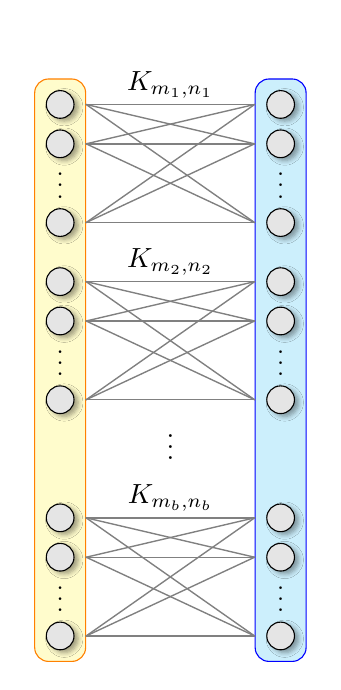
\begin{tikzpicture}[every node/.style={circle,draw,minimum size=1em}, >=latex,
    myshadow/.style={
        blur shadow={shadow blur steps=5, shadow xshift=0.15em, shadow yshift=-0.1em}
    }]

    \def\Km{4}
    \def\Kn{4}
    \def\Kmskip{3}
    \def\Knskip{3}
    \def\dotsoff{0.075}

    % BLOCK 1
    \def\voff{0}
    \def\UVsep{2.8}
    \definecolor{verylightgray}{rgb}{0.9, 0.9, 0.9}
    \colorlet{verylightblue}{cyan!20}
    \colorlet{verylightyellow}{yellow!20}
    
    \foreach \i in {1,...,\Km} {
        \ifnum\i=\Kmskip
          \node[draw=none] (a\i) at (0,\voff+\dotsoff-0.5*\i) {};
        \else
            \ifnum\i=\Km
                \node[draw=none] (a\i) at (0,\voff-0.5*\i) {};
            \else
                \node[draw=none] (a\i) at (0,\voff-0.5*\i) {};
            \fi
        \fi
    }
    \foreach \i in {1,...,\Kn} {
        \ifnum\i=\Knskip
            \node[draw=none] (b\i) at (\UVsep,\voff+\dotsoff-0.5*\i) {};
        \else
            \ifnum\i=\Kn
                \node[draw=none] (b\i) at (\UVsep,\voff-0.5*\i) {};
            \else
                \node[draw=none] (b\i) at (\UVsep,\voff-0.5*\i) {};
            \fi
        \fi
    }

    % BLOCK 2
    \def\voff{-2.25}
    
    \foreach \i in {1,...,\Km} {
        \ifnum\i=\Kmskip
          \node[draw=none] (c\i) at (0,\voff+\dotsoff-0.5*\i) {};
        \else
            \ifnum\i=\Km
                \node[draw=none] (c\i) at (0,\voff-0.5*\i) {};
            \else
                \node[draw=none] (c\i) at (0,\voff-0.5*\i) {};
            \fi
        \fi
    }
    \foreach \i in {1,...,\Kn} {
        \ifnum\i=\Knskip
            \node[draw=none] (d\i) at (\UVsep,\voff+\dotsoff-0.5*\i) {};
        \else
            \ifnum\i=\Kn
                \node[draw=none] (d\i) at (\UVsep,\voff-0.5*\i) {};
            \else
                \node[draw=none] (d\i) at (\UVsep,\voff-0.5*\i) {};
            \fi
        \fi
    }

    % BLOCK 3
    \def\voff{-5.25}
    
    \foreach \i in {1,...,\Km} {
        \ifnum\i=\Kmskip
          \node[draw=none] (e\i) at (0,\voff+\dotsoff-0.5*\i) {};
        \else
            \ifnum\i=\Km
                \node[draw=none] (e\i) at (0,\voff-0.5*\i) {};
            \else
                \node[draw=none] (e\i) at (0,\voff-0.5*\i) {};
            \fi
        \fi
    }
    \foreach \i in {1,...,\Kn} {
        \ifnum\i=\Knskip
            \node[draw=none] (f\i) at (\UVsep,\voff+\dotsoff-0.5*\i) {};
        \else
            \ifnum\i=\Kn
                \node[draw=none] (f\i) at (\UVsep,\voff-0.5*\i) {};
            \else
                \node[draw=none] (f\i) at (\UVsep,\voff-0.5*\i) {};
            \fi
        \fi
    }

    % BOXES
    \node[draw=orange, rectangle, rounded corners=5pt, fit=(a1) (e4), inner sep=4pt, fill=verylightyellow] (rectU) {};
    \node[draw=blue, rectangle, rounded corners=5pt, fit=(b1) (f4), inner sep=4pt, fill=verylightblue] (rectV) {};

    % DRAW

        % BLOCK 1
    \def\voff{0}
    
    \foreach \i in {1,...,\Km} {
        \ifnum\i=\Kmskip
          \node[draw=none] (a\i) at (0,\voff+\dotsoff-0.5*\i) {\small $\vdots$};
        \else
            \ifnum\i=\Km
                \node[draw=black,fill=verylightgray,myshadow] (a\i) at (0,\voff-0.5*\i) {};
            \else
                \node[draw=black,fill=verylightgray,myshadow] (a\i) at (0,\voff-0.5*\i) {};
            \fi
        \fi
    }
    \foreach \i in {1,...,\Kn} {
        \ifnum\i=\Knskip
            \node[draw=none] (b\i) at (\UVsep,\voff+\dotsoff-0.5*\i) {\small $\vdots$};
        \else
            \ifnum\i=\Kn
                \node[draw=black,fill=verylightgray,myshadow] (b\i) at (\UVsep,\voff-0.5*\i) {};
            \else
                \node[draw=black,fill=verylightgray,myshadow] (b\i) at (\UVsep,\voff-0.5*\i) {};
            \fi
        \fi
    }
    
    \foreach \i in {1,...,\Km} {
        \foreach \j in {1,...,\Kn} {
        \ifnum\i=\Kmskip
        \else
            \ifnum\j=\Knskip
            \else
                \draw[-,draw=gray,line width=0.5,line cap=round] ($(rectU.east |- a\i)$) -- ($(rectV.west |- b\j)$);
            \fi
        \fi
        }
    }

    \node[draw=none] at ($(a1)!0.5!(b1) + (0,0.25)$) {$K_{m_1,n_1}$};

    % BLOCK 2
    \def\voff{-2.25}
    
    \foreach \i in {1,...,\Km} {
        \ifnum\i=\Kmskip
          \node[draw=none] (c\i) at (0,\voff+\dotsoff-0.5*\i) {\small $\vdots$};
        \else
            \ifnum\i=\Km
                \node[draw=black,fill=verylightgray,myshadow] (c\i) at (0,\voff-0.5*\i) {};
            \else
                \node[draw=black,fill=verylightgray,myshadow] (c\i) at (0,\voff-0.5*\i) {};
            \fi
        \fi
    }
    \foreach \i in {1,...,\Kn} {
        \ifnum\i=\Knskip
            \node[draw=none] (d\i) at (\UVsep,\voff+\dotsoff-0.5*\i) {\small $\vdots$};
        \else
            \ifnum\i=\Kn
                \node[draw=black,fill=verylightgray,myshadow] (d\i) at (\UVsep,\voff-0.5*\i) {};
            \else
                \node[draw=black,fill=verylightgray,myshadow] (d\i) at (\UVsep,\voff-0.5*\i) {};
            \fi
        \fi
    }
    
    \foreach \i in {1,...,\Km} {
        \foreach \j in {1,...,\Kn} {
        \ifnum\i=\Kmskip
        \else
            \ifnum\j=\Knskip
            \else
                \draw[-,draw=gray,line width=0.5,line cap=round] ($(rectU.east |- c\i)$) -- ($(rectV.west |- d\j)$);
            \fi
        \fi
        }
    }

    \node[draw=none] at ($(c1)!0.5!(d1) + (0,0.25)$) {$K_{m_2,n_2}$};

    % BLOCK 3
    \def\voff{-5.25}
    
    \foreach \i in {1,...,\Km} {
        \ifnum\i=\Kmskip
          \node[draw=none] (e\i) at (0,\voff+\dotsoff-0.5*\i) {\small $\vdots$};
        \else
            \ifnum\i=\Km
                \node[draw=black,fill=verylightgray,myshadow] (e\i) at (0,\voff-0.5*\i) {};
            \else
                \node[draw=black,fill=verylightgray,myshadow] (e\i) at (0,\voff-0.5*\i) {};
            \fi
        \fi
    }
    \foreach \i in {1,...,\Kn} {
        \ifnum\i=\Knskip
            \node[draw=none] (f\i) at (\UVsep,\voff+\dotsoff-0.5*\i) {\small $\vdots$};
        \else
            \ifnum\i=\Kn
                \node[draw=black,fill=verylightgray,myshadow] (f\i) at (\UVsep,\voff-0.5*\i) {};
            \else
                \node[draw=black,fill=verylightgray,myshadow] (f\i) at (\UVsep,\voff-0.5*\i) {};
            \fi
        \fi
    }
    
    \foreach \i in {1,...,\Km} {
        \foreach \j in {1,...,\Kn} {
        \ifnum\i=\Kmskip
        \else
            \ifnum\j=\Knskip
            \else
                \draw[-,draw=gray,line width=0.5,line cap=round] ($(rectU.east |- e\i.east)$) -- ($(rectV.west |- f\j)$);
            \fi
        \fi
        }
    }

    \node[draw=none] at ($(e1)!0.5!(f1) + (0,0.25)$) {$K_{m_b,n_b}$};

    \node[draw=none] at ($(e1)!0.5!(f1) + (0,1)$) {$\vdots$};
    
\end{tikzpicture}
	\caption{\textbf{Degree-preserving biclique decomposition of bipartite graph.} ??? \mbox{$\mathcal{G}_d^{(K)}=\bigoplus_b K_{m_b,n_b}$.}} \label{fig:K_mn_decomp}
\end{figure}

\subsubsection{Counting bipartite graph realisations} \label{sec:count_real}

The structure of the \textsc{ConsensusShuffle} algorithm (Alg.~\ref{alg:consensus_shuffle}) via Eq.~\eqref{eq:group_order_shuffle} affords evaluation of the order of the consensus group equivalently counting bipartite graph realisations for a given degree sequence,
\begin{align}
	|C(d)| = |\mathcal{G}_d|.
\end{align}

* The regular action of $C(d)$ affords the freedom to As all execution paths $l\in\mathcal{L}$

%Considering the $l_0\in\mathcal{L}$ execution path of Alg.~\ref{alg:consensus_shuffle}, corresponding to the identity group element $I \in C(d)$, during which no exchange operations take place, execution proceeds by iteratively eliminating the leading element of the ordered edge-set, with remaining edges unaffected, yielding the subgraph relation,
%\begin{align}
%	\mathcal{G}(\vec{E}\backslash\vec{E}_1) &\subset \mathcal{G}(\vec{E})
%\end{align}
%
%Assuming initial canonical graph assignment and sorted degree sequence (Alg.~\ref{alg:initial_assignment}), leading edge-removal equates to canonical graph assignment of the transformed degree sequence,
%\begin{align}
%	(d_U,d_V) \xrightarrow{\vec{E}\backslash\vec{E}_1} (\textsc{RedDeg}(d_U),\textsc{RedDeg}(d_V)),
%\end{align}
%where \textsc{RedDeg}($d$) decrements the leading element of $d$, truncated upon reaching zero, preserving initial ordering (Alg.~\ref{alg:count_bipartite}).
%
% which must not already belong to $E$.
%
%* Number of prohibited terms:



%* Let $d_U$ and $d_V$ denote the degree sequences for graph partitions $U$ and $V$, initially assumed to be normally ordered (decreasing by degree).

%* Assume input $E$ is in canonical form.

%* As the group action $G$ is regular we may equivalently choose any execution path and choose the identity path $l=I$ where no swaps take place under the group shuffle algorithm.

%* Acting on edge-set $E$ with leading element $e$ GroupShuffle implements:
%\begin{align}
%	|t_i(\mathrm{deg}(U),\mathrm{deg}(V)| &= |E| + 2 - d^{U}_1 - d^{V}_1 \nonumber\\
%	d^{U}_1 &= DecrementLeadDeg = d^{U}_1 - 1,\nonumber\\
%	d^{V}_1 &= d^{V}_1 - 1,\nonumber\\
%	(d^U,d^V) &= (\textsc{Trim}(d^U), \textsc{Trim}(d^V)),\nonumber\\
%	E &= E \backslash E_1 = \textsc{CanonicalGraph}(d^U,d^V),\nonumber\\
%	|E| &\to |E|-1,\nonumber\\
%\end{align}
%* Define reduced leading degree function \textsc{RLD}($d$,$i$) that subtracts a total of $i$ from vector $d$, starting at the first element, moving onto the next element when the current one reaches $0$, returning the first non-zero element of the reduced vector,
%following the convention of Eq.~\eqref{eq:subgroup_struct}. 
%* The order of the group $G$ acting on set $X$ is,
%\begin{align}
%	|C(d)| &= \prod_{i=1}^{|E|} |t_i(d)|,\\
%|t_i(d)| &= (|E|+3-i)\nonumber\\
%&-\sum_{j=1}^{\textsc{RLD}(d_U,i-1)}\mathrm{deg}(\textsc{RLD}(d_U,i-1)_j) \nonumber\\
%&-\sum_{j=1}^{\textsc{RLD}(d_V,i-1)}\mathrm{deg}(\textsc{RLD}(d_V,i-1)_j).\nonumber
%\end{align}

\begin{algorithm}[H]
\begin{algorithmic}
\Function{CountBipartiteReal}{$d$} $\to N$
	\State $d \gets \textsc{DegSort}(d)$ 	\State $N \gets 1$ \Comment{Group orbit size}
	\For{$i \gets 1 \textbf{ to } |E|$} \Comment{$O(|U|\cdot |V|)$}
		\State $t \gets \{0\leq k< i \,|\, \textsc{Transition}(i,k) = 1\}$ \Comment{$O(n)$}
	\State $N \gets N\cdot |t|$
	\EndFor
	\State \Return $N$
\EndFunction
\State
%\Function{\textsc{TransitionSpace}}{$d$} $\to N$
%	\State $|E| = \frac{1}{2}\sum_{i=1}d_i$
%	\State $N \gets |E|+i-1$
%	\State $t_U \gets \sum_{j=1}^{{d_U}'(1)} d_U'(j)$
%	\State $t_V \gets \sum_{j=1}^{{d_V}'(1)} d_V'(j)$
%	\State $N = \max(t_U,t_V)$
%	\State \Return $N$
%\EndFunction
%\State
%\Function{\textsc{RedDeg}}{$d$} $\to d$ \Comment{$O(1)$}
%	\State $d_1 \gets d_1-1$ \Comment{Decrement leading degree}
%		\If{$d_1=0$}
%			\State $d \gets d_{2:|d|}$ \Comment{Truncate leading zeros}
%		\EndIf
%	\State \Return $d$ \Comment{Reduced}
%\EndFunction
\end{algorithmic}
\caption{Count satisfying bipartite graph realisations for degree sequence $d$. \textsc{RedDeg}($d$) does not re-sort $d$, preserving its initial ordering. The elimination of zero-valued elements from $d$ equates to relabelling, but does not change the respective graph strcuture.} \label{alg:count_bipartite}
\end{algorithm}

%For 1-regular graphs we have,
%\begin{align}
%	d &= (1,\dots,1), \nonumber\\
%	\textsc{RLD}(d,i) &= 1,\,\forall\,i \nonumber\\
%	|t_i(d)| &= |E|+1-i,\nonumber\\
%	|C(d)| &= \prod_{i=1}^{|E|}(|E|+1-i)  =|E|!,
%\end{align}
%as expected for the symmetric group $S_{|E|}$.
%
%For complete bipartite graphs, $K_{m,n}$, we have,
%\begin{align}
%	d_U &= (n,\dots,n), \nonumber\\
%	d_V &= (m,\dots,m), \nonumber\\
%	RLD(d_U,i) &= n - (i\mod{n}),\nonumber\\
%	RLD(d_V,i) &= m - (i\mod{m}),\nonumber\\
%	|E| &= mn,\nonumber\\
%	|t_i(d)| &= (mn-m-n+3-i)\nonumber\\
%	&+(i\mod{n}) + (i\mod{m}).\nonumber
%\end{align}
%
%* Execution under identity operation:

\subsubsection{Sampling via random bitstreams} \label{sec:random_bitstreams}

As nodes must be in agreement on consensus assignment the \textsc{Random} functions relied upon during execution of Alg.~\ref{alg:consensus_shuffle} must evaluate consistently across network nodes, for which the established secure random bitstream $\mathcal{X}_\mathcal{N}$ (Sec.~\ref{sec:secure_shared_randomness}) is employed as per Alg.~\ref{alg:common_sampling}.

\begin{algorithm}[H]
\begin{algorithmic}
\Function{Random}{$\mathcal{X}$, $n$} $\to x$
	\Repeat
	\State $b \gets \lceil \log_2(n) \rceil$ \Comment{Minimum required number of bits}
	\State $x \gets \mathcal{X}.\mathtt{pop}(b)$ \Comment{Pop bits from bitstream}
	\Until{$x<n$} \Comment{Until $x$ is within bounds}
	\State \Return $x$
\EndFunction
\end{algorithmic}
\caption{Deterministically choose an element $x$ from $n$ choices where $\mathcal{X}$ is a secure shared random bitstream. At most \mbox{$|\mathcal{X}| \leq \lceil \log_2(n) \rceil \cdot \log_2(1/\delta)$} bits are required to ensure success with probability \mbox{$p\geq 1-\delta$}.} \label{alg:common_sampling}
\end{algorithm}

While this function is deterministic it is not guaranteed to halt if $n\neq 2^b$ where $b\in\mathbb{Z}^+$. The success probability for a single iteration of the repeat block in Alg.~\ref{alg:common_sampling} is,
\begin{align}
	p_1(n) = \frac{n}{2^{\lceil \log_2(n) \rceil}} \geq \frac{1}{2},
\end{align}
where the worst-case lower-bound of $p=1/2$ arises when \mbox{$n=2^b+1$} for \mbox{$b\gg 1$},
\begin{align}
	p_1(2^b+1) &= \frac{1}{2} + \frac{1}{2^{b+1}},\nonumber\\
	\lim_{b\to\infty} p_1(2^b+1) &= \frac{1}{2}.
\end{align}
With $m$ rounds the success probability is,
\begin{align}
	p_m(n) = 1-(1-p_1)^m > 1-\frac{1}{2^m}.
\end{align}
Limiting the probability of failure to $\delta=1/2^m$ requires at most,
\begin{align}
	m \geq \log_2(1/\delta),
\end{align}
rounds. Hence, the worst-case consumption of random bits is,
\begin{align}
	|\mathcal{X}^{(n)}| \leq \lceil \log_2(n) \rceil \cdot \log_2(1/\delta).
\end{align}
The respective number of bits required to address all elements of the symmetric group, $S_n$, with $\delta$-likelihood of failure for all calls to \textsc{Random}$(\mathcal{X},\cdot)$ is,
\begin{align}
	|\mathcal{X}|^{(S_n)} &= \sum_{i=1}^n |\mathcal{X}^{(i)}| \nonumber\\
	&= \log_2(1/\delta) \cdot \sum_{i=1}^n \lceil\log_2(i)\rceil \nonumber\\
	&\approx \log_2(1/\delta) \cdot \log_2(n!),
\end{align}
an effective $\log_2(1/\delta)$ multiplicative overhead on the scaling relationship shown in Fig.~\ref{fig:bits_permutations}.

\subsubsection{Initial assignment} \label{sec:initial_graph_assignment}

\begin{figure}[!htb]
	\centering
	\begin{tikzpicture}[genericStyle]
    \def\N{10}
    \def\nskip{7}
    \def\conn{5}
    \def\UVsep{5}
    
    \foreach \i in {1,...,\N} {
        \ifnum\i=\nskip
          \node[draw=none] (a\i) at (0,-\i) {\LARGE $\vdots$};
        \else
            \ifnum\i=\N
                \node[nodeUStyle] (a\i) at (0,-\i) {}; % $u_m$
            \else
                \node[nodeUStyle] (a\i) at (0,-\i) {}; % $u_{\i}$
            \fi
        \fi
    }
    \foreach \i in {1,...,\N} {
        \ifnum\i=\nskip
            \node[draw=none] (b\i) at (\UVsep,-\i) {\LARGE $\vdots$};
        \else
            \ifnum\i=\N
                \node[nodeVStyle] (b\i) at (\UVsep,-\i) {}; % $v_n$
            \else
                \node[nodeVStyle] (b\i) at (\UVsep,-\i) {}; % $v_{\i}$
            \fi
        \fi
    }
    
     \foreach \i in {1,...,\N} {
     	\foreach \j in {1,...,\N} {
               \ifnum\i=\nskip
                \else
                	\ifnum\j=\nskip
                    \else
                        \draw[graphNonEdgeStyle] ($(a\i.east)$) -- ($(b\j.west)$);
                    \fi
                \fi
        }
    }

    
    \foreach \i in {1,...,\N} {
        \foreach \offset in {1,...,\conn} {
            \pgfmathtruncatemacro{\target}{mod(\i+\offset-2,\N)+1}
                \ifnum\i=\nskip
                \else
                \ifnum\target=\nskip
                    \else
                        \draw[graphEdgeStyle] ($(a\i.east)$) -- ($(b\target.west)$);
                    \fi
                \fi
        }
    }
    
  	\foreach \j in {1,...,\conn} {
                        \draw[-,redHighlightColor,line width=2,line cap=round] ($(a1.east)$) -- ($(b\j.west)$);
        }

    \node[draw=none] at ($(a1)!0.5!(b1) + (0,0.3)$) {$\mathcal{G}_{n,d}$};

    \coordinate (bracetop) at ($(b1.east) + (1em,0)$);
    \coordinate (bracetopin) at ($(bracetop) + (-0.1,0)$);
    \coordinate (bracebott) at ($(b\conn.east) + (1em,0)$);
    \coordinate (bracebottin) at ($(bracebott) + (-0.1,0)$);
    \draw[redHighlightColor, line width=1.5] (bracetopin) -- (bracetop) -- (bracebott) -- (bracebottin);

        \node[draw=none] at ($(bracetop)!0.5!(bracebott) + (3.5em,0)$) {$d=N(r/p,\varepsilon)$};
\end{tikzpicture}
	\caption{\textbf{Uniform bidding initial assignment graph.} \mbox{$\mathcal{G}_{n,d}$ has $n$ nodes and $n$ consensus sets, all with degree $d$.}}\label{fig:butterfly_graph}
\end{figure}

\begin{figure}[!htb]
	\centering
	\resizebox{0.31\columnwidth}{!}{
    \begin{tikzpicture}[genericStyle]
        \def\N{6}
        \def\nskip{8}
        \def\conn{1}
        \def\UVsep{2.8}

        \foreach \i in {1,...,\N} {
                \ifnum\i=\nskip
                    \node[draw=none] (a\i) at (0,-\i) {\LARGE $\vdots$};
                \else
                    \ifnum\i=\N
                        \node[nodeNetworkStyle] (a\i) at (0,-\i) {}; % $u_m$
                    \else
                        \node[nodeNetworkStyle] (a\i) at (0,-\i) {}; % $u_{\i}$
                    \fi
                \fi
            }
        \foreach \i in {1,...,\N} {
                \ifnum\i=\nskip
                    \node[draw=none] (b\i) at (\UVsep,-\i) {\LARGE $\vdots$};
                \else
                    \ifnum\i=\N
                        \node[nodeConsensusStyle] (b\i) at (\UVsep,-\i) {}; % $v_n$
                    \else
                        \node[nodeConsensusStyle] (b\i) at (\UVsep,-\i) {}; % $v_{\i}$
                    \fi
                \fi
            }


        \foreach \i in {1,...,\N} {
                \foreach \j in {1,...,\N} {
                        \ifnum\i=\nskip
                        \else
                            \ifnum\j=\nskip
                            \else
                                \draw[graphNonEdgeStyle] ($(a\i.east)$) -- ($(b\j.west)$);
                            \fi
                        \fi
                    }
            }

        \foreach \i in {1,...,\N} {
                \foreach \offset in {1,...,\conn} {
                        \pgfmathtruncatemacro{\target}{mod(\i+\offset-2,\N)+1}
                        \ifnum\i=\nskip
                        \else
                            \ifnum\target=\nskip
                            \else
                                \draw[graphEdgeStyle] ($(a\i.east)$) -- ($(b\target.west)$);
                            \fi
                        \fi
                    }
            }

        \node[draw=none] at ($(a1)!0.5!(b1) + (0,0.5)$) {\large $\mathcal{G}_{6,1}$};
    \end{tikzpicture}
}
	\hfill
	\resizebox{0.31\columnwidth}{!}{
\begin{tikzpicture}[genericStyle]
    \def\N{6}
    \def\nskip{8}
    \def\conn{3}
    \def\UVsep{2.8}
    
    \foreach \i in {1,...,\N} {
        \ifnum\i=\nskip
          \node[draw=none] (a\i) at (0,-\i) {\LARGE $\vdots$};
        \else
            \ifnum\i=\N
                \node[nodeUStyle] (a\i) at (0,-\i) {}; % $u_m$
            \else
                \node[nodeUStyle] (a\i) at (0,-\i) {}; % $u_{\i}$
            \fi
        \fi
    }
    \foreach \i in {1,...,\N} {
        \ifnum\i=\nskip
            \node[draw=none] (b\i) at (\UVsep,-\i) {\LARGE $\vdots$};
        \else
            \ifnum\i=\N
                \node[nodeVStyle] (b\i) at (\UVsep,-\i) {}; % $v_n$
            \else
                \node[nodeVStyle] (b\i) at (\UVsep,-\i) {}; % $v_{\i}$
            \fi
        \fi
    }
    
    
     \foreach \i in {1,...,\N} {
     	\foreach \j in {1,...,\N} {
               \ifnum\i=\nskip
                \else
                	\ifnum\j=\nskip
                    \else
                        \draw[graphNonEdgeStyle] ($(a\i.east)$) -- ($(b\j.west)$);
                    \fi
                \fi
        }
    }
    
    \foreach \i in {1,...,\N} {
        \foreach \offset in {1,...,\conn} {
            \pgfmathtruncatemacro{\target}{mod(\i+\offset-2,\N)+1}
                \ifnum\i=\nskip
                \else
                \ifnum\target=\nskip
                    \else
                        \draw[graphEdgeStyle] ($(a\i.east)$) -- ($(b\target.west)$);
                    \fi
                \fi
        }
    }

    \node[draw=none] at ($(a1)!0.5!(b1) + (0,0.5)$) {\large $\mathcal{G}_{6,3}$};
\end{tikzpicture}
}
	\hfill
	\resizebox{0.31\columnwidth}{!}{
\begin{tikzpicture}[genericStyle]
    \def\N{6}
    \def\nskip{8}
    \def\conn{6}
    \def\UVsep{2.8}
    
    \foreach \i in {1,...,\N} {
        \ifnum\i=\nskip
          \node[draw=none] (a\i) at (0,-\i) {\LARGE $\vdots$};
        \else
            \ifnum\i=\N
                \node[nodeUStyle] (a\i) at (0,-\i) {}; % $u_m$
            \else
                \node[nodeUStyle] (a\i) at (0,-\i) {}; % $u_{\i}$
            \fi
        \fi
    }
    \foreach \i in {1,...,\N} {
        \ifnum\i=\nskip
            \node[draw=none] (b\i) at (\UVsep,-\i) {\LARGE $\vdots$};
        \else
            \ifnum\i=\N
                \node[nodeVStyle] (b\i) at (\UVsep,-\i) {}; % $v_n$
            \else
                \node[nodeVStyle] (b\i) at (\UVsep,-\i) {}; % $v_{\i}$
            \fi
        \fi
    }
    
    
     \foreach \i in {1,...,\N} {
     	\foreach \j in {1,...,\N} {
               \ifnum\i=\nskip
                \else
                	\ifnum\j=\nskip
                    \else
                        \draw[graphNonEdgeStyle] ($(a\i.east)$) -- ($(b\j.west)$);
                    \fi
                \fi
        }
    }
    
    \foreach \i in {1,...,\N} {
        \foreach \offset in {1,...,\conn} {
            \pgfmathtruncatemacro{\target}{mod(\i+\offset-2,\N)+1}
                \ifnum\i=\nskip
                \else
                \ifnum\target=\nskip
                    \else
                        \draw[graphEdgeStyle] ($(a\i.east)$) -- ($(b\target.west)$);
                    \fi
                \fi
        }
    }

    \node[draw=none] at ($(a1)!0.5!(b1) + (0,0.5)$) {\large $\mathcal{G}_{6,6}=K_{6,6}$};
\end{tikzpicture}
}
	\caption{\textbf{Uniform bidding initial assignment graph.} \mbox{$\mathcal{G}_{n,d}$} has $n$ nodes and $n$ consensus sets, all with degree $d$, where \mbox{$d\leq n$}. For \mbox{$n=d$} we obtain the complete bipartite graph \mbox{$\mathcal{G}_{n,n}=K_{n,n}$.}}\label{fig:butterfly_graph_comp}
\end{figure}

Uniformly sampling consensus allocation requires applying sampled consensus group transformations (Alg.~\ref{alg:consensus_shuffle}) to an initial satisfying graph assignment (Fig.~\ref{fig:bipartite_map}) --- a solution to the \emph{bipartite realisation problem}. Via the Gale-Ryser theorem \cite{Gale1957, Ryser1957}, realisable bipartite graphs (those with \emph{bigraphic} degree sequences) demands,
\begin{align} \label{eq:bipartite_real}
	\sum_{i=1}^{|U|} \mathrm{deg}(u_i) &= \sum_{j=1}^{|V|} \mathrm{deg}(v_j),\\
	\sum_{i=1}^k \mathrm{deg}(u_i) &\leq \sum_{j=1}^{|V|} \min(\mathrm{deg}(v_j),k),\,\forall\, k\in\{1,\dots,|V|\},\nonumber
\end{align}
where the second constraint assumes $U$ and $V$ are ordered decreasingly by degree. Realisable bipartite graphs may be efficiently realised using the Havel-Hakimi algorithm \cite{Havel1955, Hakimi62}, shown in Alg.~\ref{alg:initial_assignment}, which we employ for initial canonical graph assignment.

%\footnote{In retrospect, the probability constraints imposed by Eq.~\eqref{eq:prob_cons} imply Alg.~\ref{alg:initial_assignment} directly affords a less sophisticated uniform sampling algorithm by replacing the inner for-loop with uniform selection of $\mathrm{deg}(u)$ vertices $v$ where \mbox{$\mathrm{deg}(v)>0$},\begin{align}\vec{v}'\gets\textsc{ChooseRandom}(\{\vec{v}_j\,|\, \mathrm{deg}(\vec{v}_j)>0\}_j,\mathrm{deg}(u)).\end{align}The author has a preference for the approach presented in the main text.}.

The simplest bidding format for ensuring realisable consensus assignment is \emph{uniform bidding} where all nodes request a single consensus set of size $|\mathcal{C}|$, and all vertices have constant degree,
\begin{align}
	\mathrm{deg}(u) = \mathrm{deg}(v)= |\mathcal{C}|,\,\,\forall\, u\in U, v\in V,
\end{align}
which is realisable as per Eq.~\eqref{eq:bipartite_real} if and only if,
\begin{align}
	|\mathcal{C}| \leq |\mathcal{N}'|,
\end{align}
where,
\begin{align}
	|U|=|V|=|\mathcal{N}'|=|\mathcal{C}|,
\end{align}
is the number of participating network nodes, equivalently the number of consensus sets. The same condition holds if all nodes request a constant number of consensus sets of uniform size.

* Policy approaches to ensure bipartite realisation:
\begin{itemize}
	\item Uniform bidding: All nodes request consensus sets of equal size as per the random subset problem.
	\item Multiple uniform bidding: Nodes request multiple consensus sets of varying size, where the arrays of consensus set sizes are uniform across users.
	\item Hierarchical bidding: ...
\end{itemize}

\begin{algorithm}[H]
\begin{algorithmic}
\Function{CanonicalGraph}{$U$, $V$, $d$} $\to E$
	\State $E \gets \{\}$ \Comment{Edge set}
	\For{$u \in U$} \Comment{$O(|U|\cdot |V|)$}
		\If{$\mathrm{deg}(u)>0$}
		\For{$v \in V$}
			\If{$\mathrm{deg}(v) > 0$}
				\State $E \gets E \cup (u,v)$ \Comment{Assign edge}
				\State $\mathrm{deg}(u) \gets \mathrm{deg}(u)-1$ \Comment{Decrement valence}
				\State $\mathrm{deg}(v) \gets \mathrm{deg}(v)-1$
				\If{$\mathrm{deg}(u) = 0$}
					\State \textbf{break}
				\EndIf
			\EndIf
		\EndFor
		\EndIf
	\EndFor
	\State $x \gets \sum_{u\in U} \mathrm{deg}(u) + \sum_{v\in V} \mathrm{deg}(v)$ \Comment{Unassigned edges}
	\If{$x\neq 0$}
		\State $E \gets \emptyset$ \Comment{Failure: unrealisable graph}
	\EndIf
	\State \Return $E$
\EndFunction
\State
\Function{DegSort}{$U$, $V$} $\to (U,V)$
	\State $U \gets \textsc{Sort}(U \,|\, \mathrm{deg}(u_i)\geq\mathrm{deg}(u_{i+1}))$ \Comment{$O(|U| \log |U|)$}
	\State $V \gets \textsc{Sort}(V \,|\, \mathrm{deg}(v_i)\geq\mathrm{deg}(v_{i+1}))$ \Comment{$O(|V| \log |V|)$}
	\State \Return $(U,V)$
\EndFunction
\end{algorithmic}
\caption{\cite{Havel1955, Hakimi62} Deterministic consensus assignment via bipartite graph realisation of a given degree sequence, with \mbox{$O(|U|\cdot |V|)$} time-complexity.} \label{alg:initial_assignment}
\end{algorithm}

Fig.~\ref{fig:butterfly_graph}
\begin{align}
	\mathcal{G}_{n,d}:\, e_{i,j} = \begin{cases} 
      1, & (j-i)\, \mathrm{mod}\, n < d\\
      0, & \mathrm{otherwise} 
   \end{cases},
\end{align}


\section{Distributed consensus networks} \label{sec:DCN}

\subsection{Model}

We consider a network of known nodes ($\mathcal{N}$) with access to a shared, public broadcast channel ($\mathcal{B}$), which nodes may \texttt{broadcast()} into and \texttt{listen()} to. The communications primitives our model relies upon are shown in Alg.~\ref{alg:comms_primitive}.

Network nodes \textsc{Bid} to participate in consensus by announcing transaction \texttt{id}s with their required consensus set size. The network forms consensus on the set of nodes and bids to accept, thereby establishing the global key $\mathcal{X}_\mathcal{N}$ which defines the assignment of consensus sets via distributed implementation of the random subset problem.

%\begin{figure}[!htb]
%	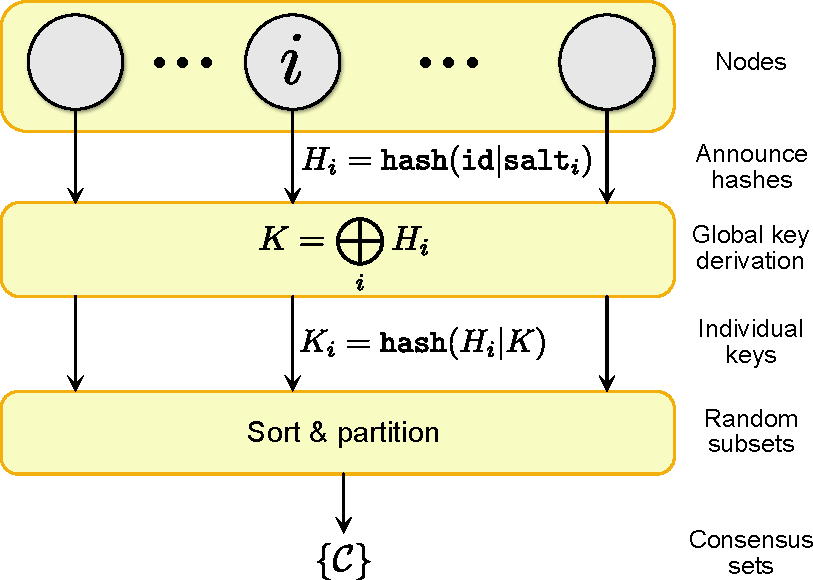
\includegraphics[width=\columnwidth]{figures/hash_based_random_subsets.pdf}
%	\caption{\textbf{Secure distributed random subset algorithm.} Nodes bid by announcing hashes $H_i$. Consensus on valid bids establishes a global key $K$, which is rehashed with all $H_i$ to obtain the local keys $K_i$ used for random assignment.}
%\end{figure}

%\section{Notation}

%$\mathcal{S}_N$, $\mathcal{S}_P$, $\mathcal{S}_C$ denote sets of network ($N$), participating ($P$) and consensus set ($C$) nodes.

%$\mathcal{B}$ denotes a common broadcast channel, observed by all nodes, into which all nodes may announce messages.

%A distributed consensus network comprises a set of known nodes accessing a shared broadcast channel, $\mathcal{B}$. There are two types of nodes, consensus ($\mathcal{C}$) and validator ($\mathcal{V}$) nodes, both bidding to participate in consensus on a bundle of transactions, for which they are offered a reward upon completion.
%
%All nodes possess the same list of public signatures of every node in the network, defining the consensus and validator pools. Nodes are allocated to consensus sets via distributed implementation of the random subset problem. Consensus nodes $\mathcal{C}$ are allocated to forming consensus on statements presented by the market, while validator nodes $\mathcal{V}$ are responsible for enforcing compliance of consensus nodes.
%
%To incentivise compliance with the protocol, nodes initially stake a deposit to participate, returned upon completing the protocol.

%\subsection{Communications primitives}

\begin{algorithm}[H]
\begin{algorithmic}
\Function{Announce}{$\mathtt{node}$, $\mathtt{statement}$}
	\State $\mathtt{message} = \textsc{Sign}(\mathtt{node}, \mathtt{statement})$
	\State $\mathcal{B} \gets \mathcal{B} \cup \mathtt{message}$ \Comment{Broadcast}
\EndFunction
\State
\Function{CommitReveal}{$\mathtt{node}$, $\mathtt{statement}$}
	\State $\mathtt{salt} = \textsc{Random}(\{0,1\}^n)$
	\State \LComment{1. Commit hash}
	\State \textsc{Announce}($\mathtt{node}$, $\textsc{Hash}(\mathtt{statement}|\mathtt{salt})$)
	\State \LComment{2. Reveal pre-image}
	\State \textsc{Announce}($\mathtt{node}$, $\mathtt{message}|\mathtt{salt}$)
\EndFunction
%\State
%\Function{Reveal}{$\mathtt{node}$, $\mathtt{statement}$}
%	\State \textsc{Announce}($\mathtt{node}$, $\mathtt{salt(statement)}$)
%\EndFunction
\end{algorithmic}	
\caption{Communications primitives, where $\mathcal{B}$ denotes the shared broadcast channel and numbers denote distinct synchronous steps.} \label{alg:comms_primitive}
\end{algorithm}

\subsection{Protocol}

\begin{figure}[!htb]
	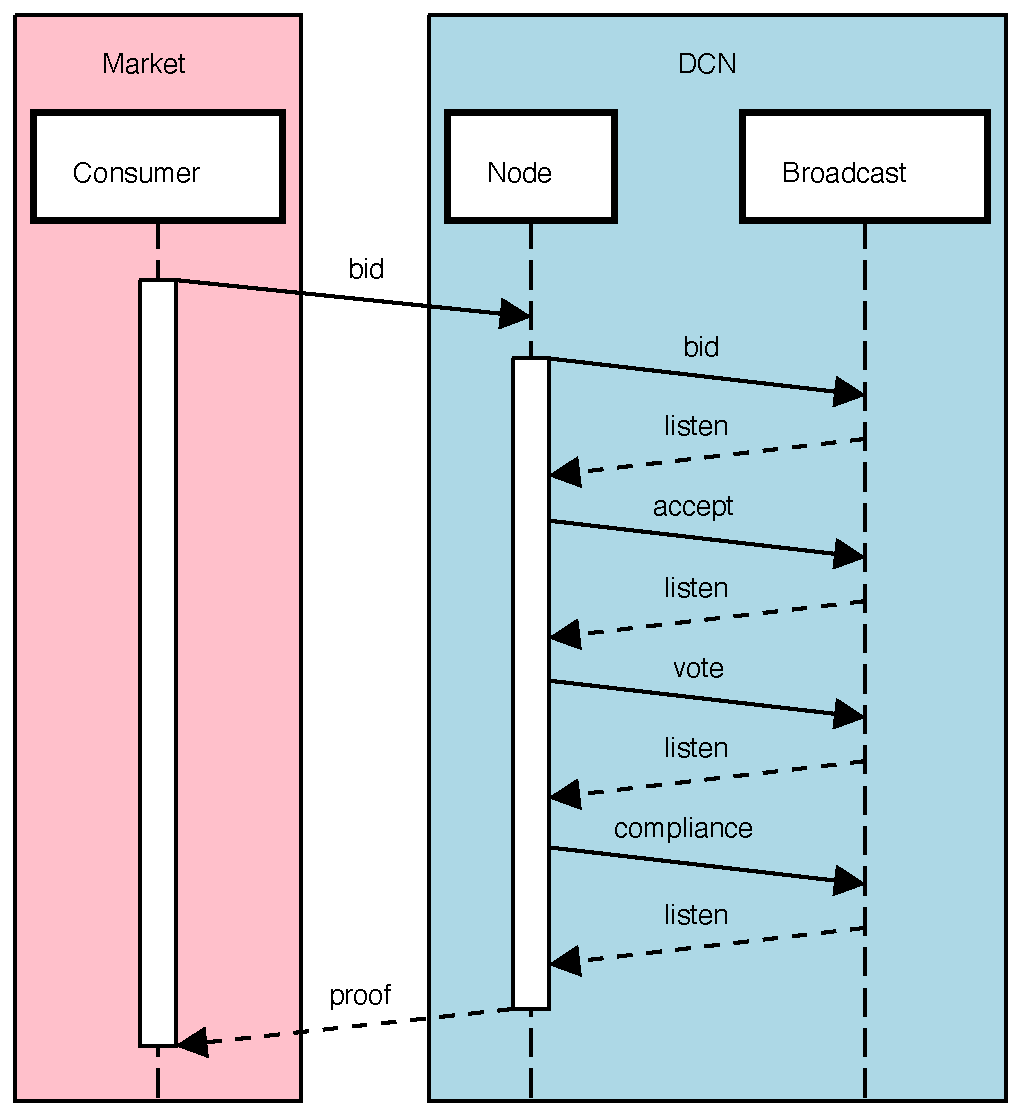
\includegraphics[width=\columnwidth]{figures/sequence_diagram.pdf}	
	\caption{\textbf{DCN protocol sequence diagram.} (blue) DCN internal network. (red) External consensus market.} \label{fig:sequence_diagram}
\end{figure}

The DCN protocol is synchronous with the following steps for each network node $i\in\mathcal{N}$:
\begin{enumerate}
	\item \textsc{Bid}: Nodes ($i$) bid to participate by presenting a set of requests ($j$) for consensus sets of given sizes ($|\mathcal{C}_{i,j}|$),
		\begin{align}
			\mathcal{R}_{i,j} &= (\mathtt{id}_{i,j},|\mathcal{C}_{i,j}|),\nonumber\\
			\mathcal{R}_i &= \bigcup_j \mathcal{R}_{i,j},
		\end{align}
		and stating recognised network nodes via the set of their public keys ($\mathtt{PubKey}_j$),
		\begin{align}
			\mathcal{N}^{(i)} = \{\mathtt{PubKey}_j\}.
		\end{align}
		All nodes broadcast (commit-reveal):
		\begin{align}
			\mathcal{B} \gets (\mathcal{R}_i, \mathcal{N}^{(i)}).
		\end{align}
	\item \textsc{Accept}: Observing the broadcast channel $\mathcal{B}$, all nodes infer the accepted network state, bids and participating nodes ($\mathcal{N}'$),
		\begin{align}
			\mathcal{B} &\to (\tilde{\mathcal{R}},\tilde{\mathcal{N}}',\tilde{\mathcal{N}}),\nonumber\\
			\tilde{\mathcal{N}} &= \textsc{MajorityVote}(\{\mathcal{N}^{(j)}\}),\nonumber\\
			(\tilde{\mathcal{R}},\tilde{\mathcal{N}}') &= \textsc{Accept}(\{\mathcal{R}_j\}),
		\end{align}
		where \textsc{Accept}($\cdot$) is a network-agreed deterministic function, and ${}^\sim$ denotes values inferred from the broadcast channel.
		
		In this step consensus is performed at the network level where all network nodes form a single consensus set, requiring that participants form a network majority,
		\begin{align}
			|\mathcal{N}'|>\frac{|\mathcal{N}|}{2}.
		\end{align}
		All other votes in the protocol are conducted at the level of assigned consensus sets.
%	 Nodes vote on accepted bids in accordance with network policy, defining the set of participating nodes $\mathcal{S}_P$ and bids $\mathcal{R}$. Agreement on accepted bids implies the established global key $X_{\mathcal{S}_P}$ and assignment of random subsets.
	%\item $\mathcal{N}_i\in\{\mathtt{public\_key}\}^{|\mathcal{S}|}$, $\mathcal{P}_i\in\{0,1\}^{|\mathcal{S}|}$: List of public-keys of all recognised network nodes, and associated binary vector of recognised participants.
	\item \textsc{Consensus}: The global key $\mathcal{X}_{\mathcal{N}}$ is implied by the accepted parameters (Sec.~\ref{sec:secure_shared_randomness}) as is the network's allocation to consensus sets via the random subset algorithm (Sec.~\ref{alg:random_subset}). 
		\begin{align}
			\mathcal{B} &\to \mathcal{X}_{\mathcal{N}} \to \{\mathcal{C}\}.
		\end{align}
		Participating nodes vote (commit-reveal) on their assigned consensus requests,
		\begin{align}
			\mathcal{B} &\gets \textsc{Vote}_i(\tilde{\mathcal{R}}).
		\end{align}
	\item \textsc{Compliance}: Nodes vote (announce) on the compliance of participating nodes and reveal the time-of-receipt of all broadcast messages associated with the respective consensus'. Compliant nodes follow all required protocol steps, are in agreement with the majority on all votes, where timestamps (time-of-receipt) of all announcements are within the network's $\delta$ threshold.
		\begin{align}
			\mathcal{B} \gets \textsc{CompliantSet}_i(\mathcal{N}).
		\end{align}
	\end{enumerate}
% , \textsc{Timestamp}_i(\mathcal{B})
 
%A synchronous protocol for solving the random subset problem is shown in Alg.~\ref{alg:consensus_sets}, where numbers indicate the synchronous steps.

%Nodes must remain compliant with the protocol to secure return of their stake. This requires nodes to be in agreement with the majority on all votes. For validator nodes this additionally requires their timestamps of messages in the broadcast channel be consistent with consensus time, where all validator nodes are required to timestamp all messages in the broadcast channel.

%The consensus time for a given message is taken to be the median of all reported timestamps. The median exhibits the property that if a majority of timestamps are within $\delta$ of the median, no action by an adversarial minority is able to undermine this. Hence, consensus time is dictated by the majority. In a setting where non-compliance is penalised, this incentivises consensus time towards accuracy, allowing the protocol to self-synchronise, independent of an external time reference.

%\begin{algorithm}[!htb]
%\begin{algorithmic}
%\Function{ConsensusSets}{$\mathcal{S}$, $\{|C|\}$, $\{\texttt{id}\}$} $\to \{\mathcal{C}\}$
%	\State \LComment{1. Nodes bid to participate}
%	\For{$i\in \mathcal{P}$}
%		\LComment{Announce salted hash of \texttt{header}}
%		\State $H_i \gets \textsc{Commit}(i, \mathtt{header})$
%	\EndFor
%%	\State
%%	\State \LComment{2. Validators commit recognised bids}
%%	\For{$j\in \mathcal{S}_V$} 
%%		\State $B_j \gets \textsc{Commit}(j, \textsc{RecognisedBids}(j))$
%%	\EndFor
%	\State
%	\State \LComment{2. Nodes form consensus on valid bidders}
%	\State $A \gets \textsc{ConsensusParticipants}(\mathcal{P})$
%	\State
%	\State \LComment{3. Assign consensus sets}
%	\State $K = \textsc{Hash}(\textsc{Sort}(\bigcup_{i\in A} H_i))$ \Comment{Shared randomness}
%	\For{$i\in A$}
%	\State $K_i \gets \textsc{Hash}(H_i|K)$ \Comment{Randomised local keys}
%	\EndFor
%	\State $\mathtt{sorted} \gets \textsc{Sort}(A, \{K_i\})$ \Comment{Sort nodes by local keys}
%	\State $\mathcal{C} \gets \textsc{Partition}(\mathtt{sorted}, N_C)$ \Comment{Partition into sets}
%	\State \Return $\mathcal{C}$
%\EndFunction
%\end{algorithmic}
%\caption{Distributed synchronous protocol for hash-based random subsets.} \label{alg:consensus_sets}
%\end{algorithm}

%\begin{algorithm}[!htb]
%\begin{algorithmic}
%\Function{Compliance}{$\mathcal{S}$} $\to \tilde{\mathcal{S}}$
%	\State $\tilde{\mathcal{S}} \gets \{\}$ \Comment{Compliant nodes}
%	\For{$j\in \mathcal{S}$}
%		\State $\mathtt{compliant} \gets \mathtt{true}$
%		\State
%		\State \LComment{Nodes must agree with majority votes}
%		\State $\mathcal{C} \gets \textsc{ConsensusParticipants}(\mathcal{V})$
%		\State $\mathcal{C}_j \gets \textsc{RecognisedParticipants}(j)$
%		\If{$\mathcal{C} \neq \mathcal{C}_j$}
%			\State $\mathtt{compliant} \gets \mathtt{false}$
%		\EndIf
%		\State
%		\State \LComment{Nodes must conform with consensus time}
%		\For{$\mathtt{message} \in \textsc{AllMessages}$}
%		\State $t$ = \textsc{Timestamp}($j$, $\mathtt{message}$)
%		\If{$|t -\textsc{ConsensusTime}(\mathcal{V},\mathtt{message})|\geq\delta$}
%			\State $\mathtt{compliant} \gets \mathtt{false}$
%		\EndIf
%		\EndFor
%		\State
%		\If{$\mathtt{compliant}$}
%			\State $\tilde{\mathcal{V}} \gets \tilde{\mathcal{V}} \cup j$
%		\EndIf
%	\EndFor
%	\State \Return $\tilde{\mathcal{V}}$
%\EndFunction
%\end{algorithmic}	
%\caption{Compliance checking.} \label{alg:compliance}
%\end{algorithm}

%\subsubsection{Consensus load allocation}
%
%During bidding nodes ($i$) request some number of independent consensus sets $|\mathcal{R}_i|$, each of size $|\mathcal{C}_{i,j}|$, with net requested consensus load,
%\begin{align}
%	|\mathcal{C}_i| = \sum_{j=1}^{|\mathcal{R}_i|} |\mathcal{C}_{i,j}|.
%\end{align}
%As all consensus sets are subsets of the network, nodes cannot be assigned to a given consensus set more than once, imposing the constraint,
%\begin{align}
%	|\mathcal{C}_{i,j}|\leq |\mathcal{S}_P|.
%\end{align}
%The total consensus load is,
%\begin{align}
%	|\mathcal{C}| = \sum_{i=1}^{|\mathcal{S}_P|} |\mathcal{C}_{i,j}|,
%\end{align}
%which must be allocated within a finite number of network rounds ($N_R$),
%\begin{align}
%	|\mathcal{C}| \leq N_R \cdot |\mathcal{S}_P|.
%\end{align}
%
%In accordance with network-defined policy some subset of bids are \textsc{Accept}ed to bound total consensus load and ensure fairness in access to consensus.

\subsubsection{Network participant acceptance}

??? TO DO

Decomposing a network into honest and dishonest nodes,
\begin{align}
	\mathcal{N} &= \mathcal{N}_H \cup \mathcal{N}_D,\nonumber\\
		|\mathcal{N}| &= |\mathcal{N}_H| + |\mathcal{N}_D|,
\end{align}
the ratios of malicious ($r$) and participating ($p$) nodes in the network are,
\begin{align}
	r = \frac{|\mathcal{N}_D|}{|\mathcal{N}|},\quad p = \frac{|\mathcal{N}'|}{|\mathcal{N}|},
\end{align}
where $\mathcal{N}'$ are the participating nodes,

In a worst-case adversarial model we assume all dishonest nodes are present in any participating set. The ratio of malicious nodes in the participating set is,
\begin{align}
	r' = \frac{|\mathcal{N}_D|}{p\cdot|\mathcal{N}|} = \frac{r}{p},
\end{align}
modulating the effective ratio of dishonest nodes by the ratio of participating nodes, where \mbox{$p>1/2$} and \mbox{$r<1/2$}. Maintaining \mbox{$r'<1/2$} to ensure an honest majority imposes a lower bound on the participation ratio,
\begin{align}
	p_\mathrm{min} > \mathrm{max}(2r,1/2).
\end{align}

As the effective proportion of dishonest nodes, \mbox{$r'=r/p$}, is a function of the variable network participation rate, $p$, the required consensus set size to maintain $\varepsilon$-security may be algorithmically specified upon acceptance. Now the dynamic minimum consensus set size scales as,
\begin{align}
	N_\mathrm{min}(r/p,\varepsilon),
\end{align}
shown in Fig.~\ref{fig:P_M_p}.

\begin{figure}
	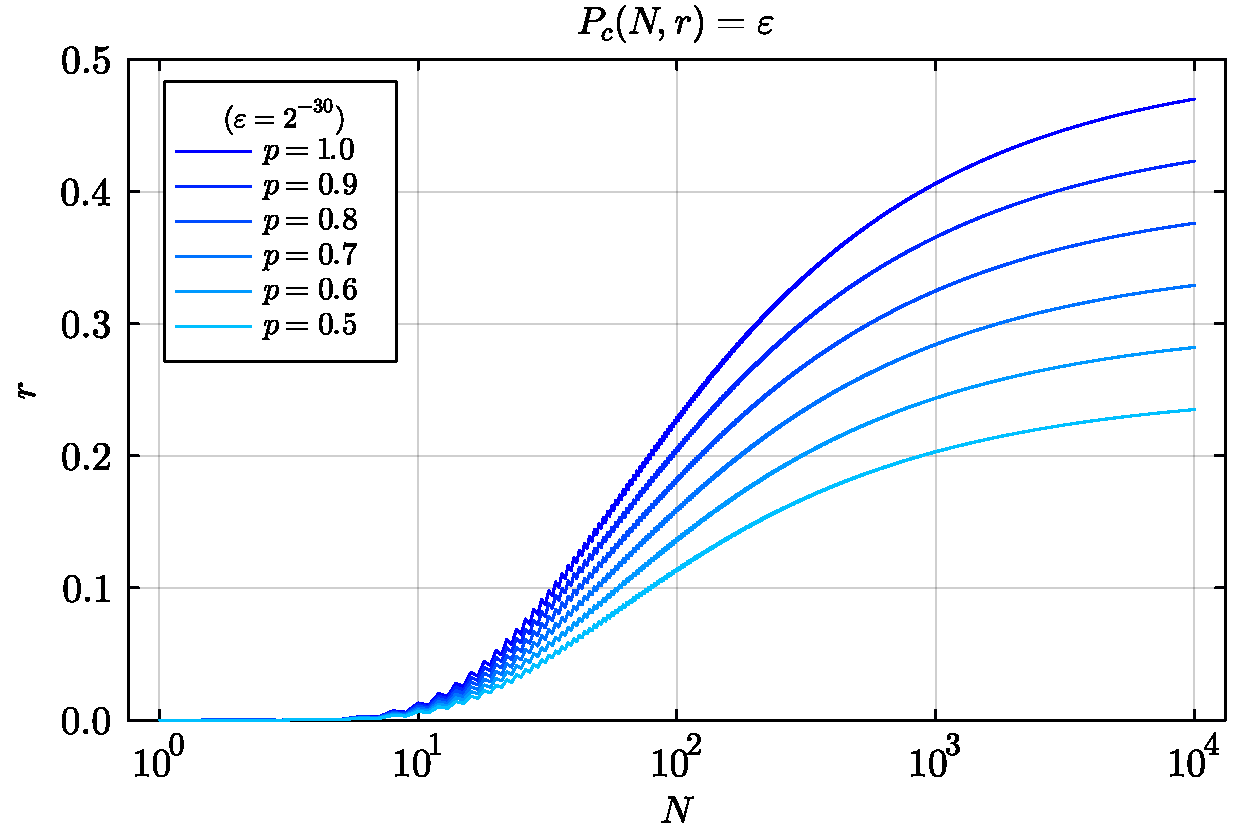
\includegraphics[width=\columnwidth]{figures/majority_prob_p.pdf}\\
	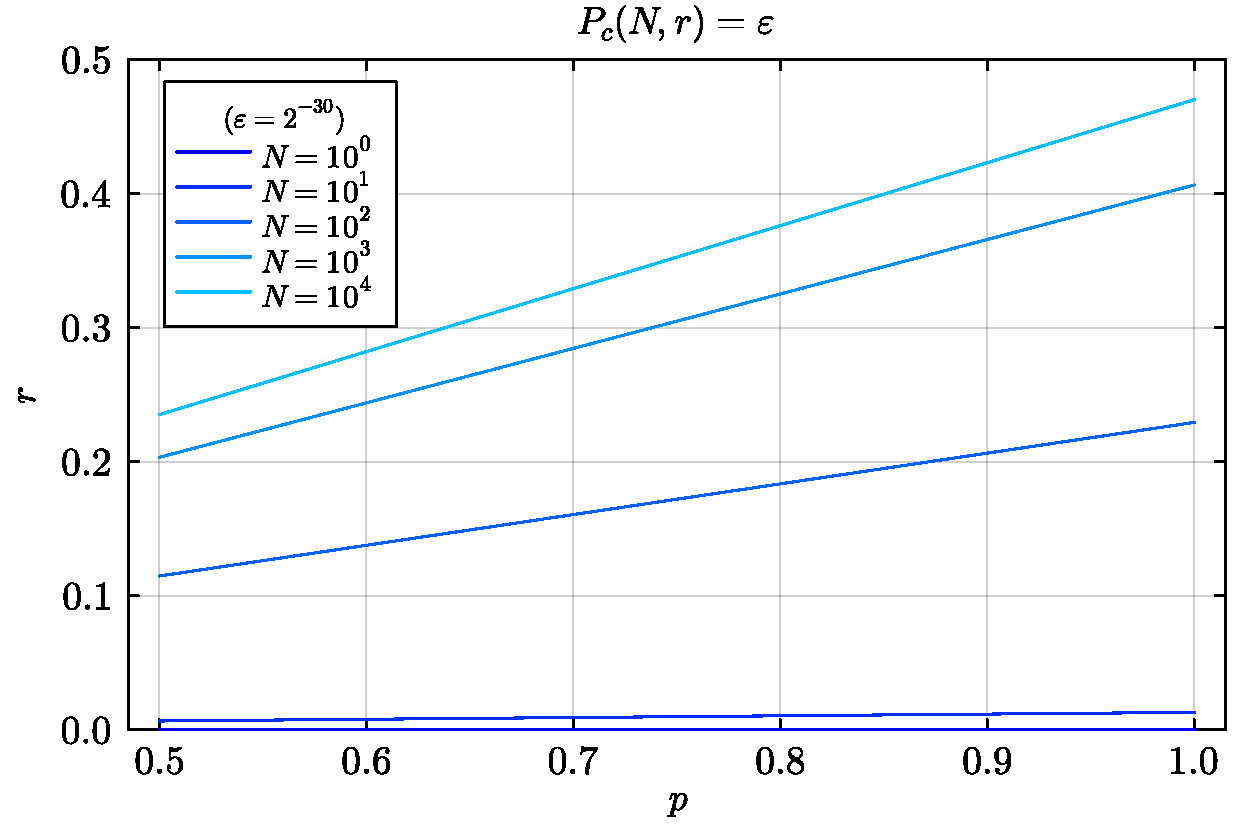
\includegraphics[width=\columnwidth]{figures/majority_prob_N.pdf}
	\caption{\textbf{Security tradeoffs with consensus set size and variable network participation.} \mbox{$P_c(N,r/p)\leq\varepsilon$} is the probability that dishonest nodes within a random subset of size $N$ form a false-majority when the proportion of dishonest nodes is \mbox{$r'=r/p$}, with network participation $p$. Shown for constant \mbox{$\varepsilon=2^{-30}$}, where the \mbox{$p=1$} curve corresponds to the respective curve in Fig.~\ref{fig:P_M}.}\label{fig:P_M_p}
\end{figure}

\subsection{Consensus time}

* ??? TODO

To enforce synchronisation of the protocol compliance requires nodes' broadcast messages to satisfy timing constraints under majority vote. To establish majority vote outcomes on the timing of messages we introduce \emph{consensus time}, given by the median of the reported times of receipt of messages (Alg.~\ref{alg:consensus_time}).

\begin{algorithm}[H]
\begin{algorithmic}
\Function{ConsensusTime}{$\mathcal{C}$, \texttt{message}} $\to \mathbb{R}$
	\State $\texttt{times} \gets \{\textsc{TimeOfReceipt}(i,\texttt{message})$\}$_{i\in\mathcal{C}}$
	\State \Return \textsc{Median}(\texttt{times})
\EndFunction
\end{algorithmic}	
\caption{Consensus time of a broadcast message is given by the median of the times of receipt reported by nodes.} \label{alg:consensus_time}
\end{algorithm}

Consensus time exhibits the property that if for any majority of consensus nodes,
\begin{align}
	|t_i - \textsc{ConsensusTime}(\mathcal{C},\texttt{message})|	\leq \delta,
\end{align}
no reported $t_i$ for the remaining minority can shift consensus time by more than $\delta$, making consensus time robust against minority manipulation. Consensus time may therefore be utilised as an implied majority vote on nodes' timing compliance,
\begin{align}
	\textsc{MajorityVote}(\mathcal{C}, \textsc{Compliant}(\texttt{message})).
\end{align}
Let the worst-case network latencies be,
\begin{align}
	\tau_\mathrm{max} = \max_{i,j\in\mathcal{N}}(\tau_{i,j}),
\end{align}
where $\tau_{i,j}$ is the matrix of point-to-point latencies between nodes $i$ and $j$. A message broadcast at time $t_B$ will be received by all network nodes by at latest $t_B+\tau_\mathrm{max}$.
By majority vote, the latest time at which a message could have been broadcast is,
\begin{align}
	t_B \leq \textsc{ConsensusTime}(\mathcal{C},\texttt{message}) - \tau_\mathrm{max}.
\end{align}

Ensuring majority votes on consensus time are well-defined requires,
\begin{align}
	\delta \geq \frac{\tau_\mathrm{max}}{2}.
\end{align}

%\begin{align}
%	\textsc{MajorityVote}(\mathcal{C}, \textsc{TransmissionTime}(\texttt{message}))
%\end{align}

%\subsection{Design considerations}
%
%* Scaling in units of hashes and digital signatures. Computation is dominated by signing, requiring O(?). And hashes.
%
%* Multiple consensus’ assigned to nodes (inward arrows) may be parallelised.

\subsection{Proof-of-consensus} \label{sec:PoC}

The sequence of signed, broadcast announcements made by compliant network nodes ($i$) is:
\begin{itemize}
	\item $\mathcal{R}_i$: Request for consensus sets.
	\item $\mathcal{N}^{(i)}$: Public keys of all network nodes.
	\item $\textsc{Vote}_i(\tilde{\mathcal{R}}_j)$: Votes on assigned consensus'.
	\item $\textsc{Timestamp}_i(\mathcal{B})$: Time-of-receipt of broadcast messages from other nodes in the consensus set.
	\item $\textsc{CompliantSet}_i(\mathcal{C})$: Recognised compliant nodes in the consensus set.
\end{itemize}
We denote a complete set of such announcements from a given node ($i\in\mathcal{N}$) participating in consensus set $\mathcal{C}$ as,
\begin{align}
	\mathcal{P}_i(\mathcal{C}).
\end{align}
A proof-of-consensus for consensus set $\mathcal{C}$ comprises any self-consistent majority set of partial proofs,
\begin{align}
	\mathcal{P}(\mathcal{C}) = \bigcup_{i\in\textsc{Majority}(\mathcal{C})} \mathcal{P}_i(\mathcal{C}).
\end{align}
Note that while the proofs for a given consensus are not unique they are equivalent proofs of the same statement.

A proof-of-consensus in a self-contained proof system, comprising all necessary information to verify its validity.

* Variation in consensus time preserves compliance outcomes.

%During the initial bidding stage nodes announce their recognised participant set, $\mathcal{P}_i$ for node $i$..
%
%During the final compliance evaluation stage, nodes announce individual attestations
%\begin{align}
%	\mathcal{A}_i = \textsc{Sign}(\tilde{\mathcal{S}}_i)	
%\end{align}
%where $\tilde{\mathcal{S}}_i$ are the compliant nodes recognised by node $i$, $\mathcal{P}_i$ complete proof (all compliant attestations) of participants
%
%Attestation: signature system of single consensus node.
%
%Proof-of-consensus requires any majority of compliant attestations from a given consensus.
%Counts members of the powerset with size n>=Nmajority
%Sum of binomials. Half of curve.
%Number of distinct majorities amongst a set of $n$ compliant consensus nodes scales as $2^{n-1}$, a class of cryptographically equivalent proofs attesting the same statement.
%Complete proof comprises the attestations of all compliant nodes, which is unique.
%A minimal proof comprises any $m=\lfloor n/2\rfloor+1$ attestations, of which there are $\binom{n}{m}$ equivalent proofs.
%
%Proofs-of-consensus are post-blockchain primitives creating pools of PoCs from which ledgers and other applications are defined by algorithmically specified subsets as a function of time.
%
%Cryptographically equivalent proofs
%
%Structure of proofs-of-consensus: The set of proofs-of-consensus comprising exactly $m$ attestations amongst $n$ nodes comprises $\binom{n}{m}$ distinct but equivalent proofs, defining an automorphism under the symmetric group $S_n$ of node permutations. Similarly, the set of all valid proofs given by the union of $m$-proofs for all $m>n/2$ is automorphic under $S_n$.
%
%While epsilon-security assumptions guarantee the existence of at least one minimal proof, the existence of non-minimal proofs is not guaranteed, subject to the withholding of attestations which are not compliance-enforced.

%\subsection{Latency}
%
%$\delta$ upper-bounds the error in consensus-time, in turn lower-bounded by worst-case network latency. As the accuracy of consensus-time has market value, networks are incentivised towards adopting low-latency infrastructure.
%
%Following commit-reveal of consensus outcomes the final step is forming consensus on compliant participants. The existence of any majority of signatures on compliance validates the proof. As the majority are honest and compliant there is no ability for dishonest parties to withhold signatures and prevent completion of the proof. Honest nodes announcing their compliance outcomes do so in finite time, resulting in Poissonian latency in proof completion.

%Let $X_i$ be a random variable characterising the response time for node $i$ to sign final compliance on a PoC, whose expectation value is necessarily finite for honest nodes. Let $f_{X_i}(\tau)$ be the probability distribution function for $X_i$ and $F_{X_i}(\tau)$ the respective cumulative distribution function. Defining,
%\begin{align}
%Y=\max(X_1,\dots,X_m)
%\end{align}
%as the random variable characterising the time until $m$ nodes all sign compliance, we obtain,
%\begin{align}
%F_Y(\tau) &= \mathbb{P}(\max(X_1,\dots,X_m)\leq\tau)\nonumber\\
%&= \prod_{i=1}^m \mathbb{P}(X_i\leq\tau)\nonumber\\
%&= \prod_{i=1}^m F_{X_i}(\tau).
%\end{align}
%Under uniform random sampling all $X_i$ are independent and identical, yielding,
%\begin{align}
%F_Y(\tau) &= F_X(\tau)^m,
%\end{align}
%with respective probability distribution function,
%\begin{align}
%f_Y(\tau) &= \frac{d}{d\tau}F_Y(\tau) \nonumber\\
%&= m f_X(\tau) F_X(\tau)^{m-1},
%\end{align}
%and expectation value,
%\begin{align}
%\mathbb{E}(Y) &= \int_0^\infty \tau f_Y(\tau) \,d\tau.
%\end{align}
%
%Assuming individual log-normal-distributed response times we have,
%\begin{align}
%	X &= \textsc{Lognormal}(\mu,\sigma^2),\nonumber\\
%	f_X(x) &= \frac{1}{x\sigma\sqrt{2\pi}}\exp\left[-\frac{(\log{x}-\mu)^2}{2\sigma^2}\right],\nonumber\\
%	F_X(x) &= \frac{1}{2}\mathrm{erfc}\left[-\frac{\log{x}-\mu}{\sigma\sqrt{2}}\right].
%\end{align}
%
%For consensus set size $N_C$ the minimal majority is,
%\begin{align}
%m = \left\lfloor\frac{N_C}{2}\right\rfloor + 1.
%\end{align}
%
%\begin{align}
%f_Y(\tau) &= m 	
%\end{align}
%
%epsilon security against withholding.

\subsection{Network policy}

Let the network maintain its own ledger for tallying the contributed consensus workload of all network nodes, comprising an array of zero-initialised integer registers, one for each node,
\begin{align}
	\mathtt{tally}\in\mathbb{Z}^{|\mathcal{N}|}.
\end{align}
When node $i$ faithfully participates in consensus its tally register is incremented. Conversely, when requesting consensus load its tally must have sufficient balance to make the request. Under steady-state operation where nodes request what they contribute registers do not change. 

When the network accepts new nodes they are unable to immediately make consensus requests and instead make null-bids, offering to contribute load without return. This increases their tally, enabling them to make subsequent requests for consensus load. This effectively forces new nodes to buy into the network by pre-contributing load they will subsequently request.

During the \textsc{Accept} stage of the protocol, the network must also agree on the network's updated \texttt{tally} state.

* Policy: propose update.

* Accept current constitution.

%Acceptance

%Sec.~\ref{sec:ledgers}

\subsection{Resource consumption}

* Latency limits speed.

* Multiplier via independent parallel sub nets or more virtual nodes.

* Inter subnet balancing of load into single.

* Digital signature consumption.

\section{Quantum consensus networks} \label{sec:QCN}

Quantum consensus networks (QCNs) have quantum-enabled nodes, whose goal it is to form consensus on the generation of certifiable quantum randomness, an important resource in cryptography and numerous other applications.

As quantum hardware is costly compared to classical hardware it is expected that few networks will be quantum-enabled. However, they may exploit the quantum randomness provided by dedicated QCNs acting as \emph{quantum random oracles} (Sec.~\ref{sec:quantum_rand_oracles}) to inject entropy into their own global keys using \emph{entropy addition} (Sec.~\ref{sec:entropy_add}), effectively enabling classical DCNs to achieve quantum random consensus assignment.

We consider two approaches for quantum random number generation (QRNG):
\begin{itemize}
	\item Quantum key distribution (QKD): requires quantum communication but no quantum computation (Sec.~\ref{sec:QKD}).
	\item Interactive proofs of quantumness: require quantum computation but no quantum communication (Sec.~\ref{sec:IPQ}).
\end{itemize}

As these are two-party protocols, every instance may be associated with a graph edge between the respective nodes.  Random numbers associated with edges may be spoofed if both nodes collude, bypassing the need for expensive quantum resources. However, so long as at least one QRN is genuine combining them under bit-wise XOR yields a collective QRN source.

%Choosing a cyclic graph spanning all nodes, $C_n$, creates a proof-chain where the existence of a single honest player guarantees the existence of a single honest edge.

%* Same as above, but now the reported measurement outcomes are utilised as the random source, enabling quantum-random subsets.
%
%* Under randomised neighbours ff a prover node is compromised the probability it's neighbouring verifier is comprised, thereby enabling shortcutting, is:
%* P=(rN-1)/N = r-1/N (P=r for large N)
%* This proportion of adversarial nodes can bypass work in proof-of-quantumness.
%* Under collusion amongst compromised nodes:
%* Only last prover in prover-graph forced to comply: P=1/N (P=0 for large N)
%
%Directed node graph constitutes the prover graph, oppositely-directed the verifier graph.
%The prover graph is $C_n$ directed one way, the verifier graph the other.
%
%Indices provided by the global hash key define a random, directed, cyclic graph, where node i acts as verifier for node i+1 and prover to node i-1. Randomised ordering ensures the probability a neighbour is compromised is uniformly r. If this ordering could be manipulated conspiring nodes could assemble themselves into a contiguous linear subgraph where only the final prover is forced to honestly comply with the proof. The other dishonest nodes can exchange secrets to manufacture legitimate proofs of quantumness without the cost of executing the respective quantum computation. While this does not impact the integrity of the established global key, it enables bypassing the costs. Scales as 1/n cost. Not a security consideration, but one of equity. Randomised ordering enforces cost reduction of r. While inhibiting the ability to bypass cost of quantum computation is enforced by hash-randomness, the established global key seeding the allocation of random subsets is quantum-random.
%
%A fixed cycle therefore upholds quantum-random subset allocation but compromises the ability to ensure r-fairness in bypassed quantum computational cost. Taking the participating set of nodes ordered by their public keys to define a fixed cyclic graph. Randomised ordering requires point-to-point connectivity between all nodes, requiring the ability to independently route $O(n^2)$ connections. Static ordering reduces this to $O(n)$. Both exhibit $O(n)$ communications complexity and ensure secure quantum-randomness.

\subsection{Entropy sources: quantum vs. classical}

* Entropy rate
\begin{align}
	H(\mathcal{X}) = \lim_{n\to\infty} H(\mathcal{X}_n | \mathcal{X}_{n-1},\dots,\mathcal{X}_1),
\end{align}
where $H(X|Y)$ is the conditional entropy of $X$ given knowledge of $Y$.

For iid (quantum)
\begin{align}
	H(\mathcal{X}) = H(\mathcal{X}_n)
\end{align}

\subsection{Entropy addition} \label{sec:entropy_add}

The bit-wise XOR operator is a strictly non-entropy-decreasing function. For binary random variables,
\begin{align}
	\mathcal{X}_i\to\{0,1\},
\end{align}
with probability distributions,
\begin{align}
	\mathcal{X}_i:\, p_i=p_i(0)=1-p_i(1),
\end{align}
the individual binary Shannon entropies are given by,
\begin{align}
	H_2(\mathcal{X}_i) = -p_i\log_2 p_i - (1-p_i)\log_2(1-p_i),
\end{align}
where,
\begin{align}
	0 \leq H_2(\cdot) \leq 1.
\end{align}
Their combined entropy under the bit-wise XOR operation is lower-bounded by their maximum,
\begin{align}
	\max_i(\{H_2(\mathcal{X}_i)\}) \leq H_2\left(\bigoplus_i \mathcal{X}_i\right) \leq 1.
\end{align}
Hence, a random source derived from multiple sources via entropy addition is at least as random as any of them. Consequently, if any single contributing source is a genuine QRNG, so too will be their the combined source.

* What is quantum random vs classical random.

* Correlations over repeats?

* iid

* QR yields ideal Bernoulli distribution,
\begin{align}
	\mathcal{X} \sim \mathrm{Ber}(1/2).
\end{align}

* Entropy rate.

\subsection{Quantum random oracles} \label{sec:quantum_rand_oracles}

Let $\mathcal{O}(t)$ denote a dynamic set of contributing random oracles at  time $t$. We define a collective random bitstream,
\begin{align}
	\mathcal{X}_\mathcal{O}(t) = \bigoplus_{i\in\mathcal{O}(t)} \mathcal{X}_i(t),
\end{align}
whose combined entropy is bounded by,
\begin{align}
	\max_{i\in\mathcal{O}}(\{H_2(\mathcal{X}_i)\}) \leq H_2(\mathcal{X}_{\mathcal{O}}) \leq 1.
\end{align}

A classical DCN may observe a QRNG oracle and add its entropy $\mathcal{X}_\mathcal{O}$ to its own global key. For this to be secure it is required that the DCN's own global key, $\mathcal{X}_\mathcal{N}$, be committed prior to the availability of the external entropy source,
\begin{align}
	{\mathcal{\tilde X}}_\mathcal{N}(t+\Delta) = \mathcal{X}_\mathcal{N}(t) \oplus \mathcal{X}_\mathcal{O}(t+\Delta),	
\end{align}
where ${\mathcal{\tilde X}}_\mathcal{N}$ is the network's oracle-modulated global key, and \mbox{$\Delta>0$} is a pre-agreed future point in time, subsequent to commitment of the networks initially established global key, $\mathcal{X}_\mathcal{N}$.

\subsection{Quantum key distribution (QKD)} \label{sec:QKD}

Quantum key distribution (QKD) \cite{BB84, E91} enables the secure establishment of shared randomness between two parties with information theoretic security. While ordinarily utilised for secret key exchange, here we exploit not the secrecy of shared randomness but its inability to be spoofed under honest execution of the protocol.

Assuming the existence of a quantum internet \cite{RohdeQI} capable of arbitrary point-to-point entanglement routing, all node-pairs $(i,j)$ have access to an indefinite supply of maximally-entangled Bell pairs,
\begin{align}
	\ket{\Psi}_{i,j} = \frac{1}{\sqrt{2}}(\ket{0}_i\ket{0}_j+\ket{1}_i\ket{1}_j),
\end{align}
requiring full $O(n^2)$ quantum communications connectivity.

\textbf{* Stop mixing up BB84 and E91.}

For the $n$th copy of $\ket{\Psi}_{i,j}$ both nodes independently and privately choose measurement bases,
\begin{align}
	b_i(n),b_j(n)\in\{0,1\},
\end{align}
where \mbox{$b=0$} denotes the Pauli-$Z$ basis and $b=1$ the Pauli-$X$ basis, and record their associated measurement outcomes, 
\begin{align}
	m_i(n),m_j(n)\in\{0,1\}.
\end{align}
The subset of measurement outcomes where both parties operate in the same basis defines a shared random bit-string,
\begin{align}
	s_{i,j} = \{m(n)\,|\, b_i(n)=b_j(n)\}_n.
\end{align}
These post-selected bit-strings correspond identically to those provided by the E91 \cite{E91} QKD protocol. The BB84 protocol \cite{BB84} can be similarly employed with the interpretational difference that for one party $b$ and $m$ denote encoding, for the other measurement.

Physical and implementation errors reduce the otherwise perfect measurement correlations between nodes measuring in the same basis resulting in inconsistent shared strings. However, privacy amplification \cite{PrivacyAmp} may be used to reduce an imperfect random bit-string to a shorter one with higher entropy using classical post-processing.

%Using the existing hash-based global key we assign nodes to a randomly-ordered cyclic graph $C_n$, where we assume the availability of arbitrary point-to-point QKD links between all nodes in the network. For every edge in $C_n$ the two connecting nodes implement a QKD protocol, whose outcome is associated with the respective graph edge, shown in Fig.~\ref{fig:proof_chains}.
%
%The quantum-random global key is established by XORing all compliant QRNs as per Eq.~\eqref{eq:global_K}. Since cyclic graphs are connected, the existence of any honest nodes guarantees that at least one edge was honestly executed, sufficient to uphold the integrity of the established key.

%To introduce QKD-derived global keys to the protocol we introduce additional synchronous steps. Following the \textsc{Accept} stage of the classical DCN protocol, nodes are required to commit QRN strings obtained in accordance with the randomised $C_n$ graph. The \textsc{Compliance} stage of the protocol now additionally requires all committed QKD strings to pass a legitimacy test for compliance.

%In the case of entanglement-based E91 networks, both nodes measure their received qubits from distributed Bell-pairs randomly in the $X$ or $Z$ bases, where the number of samples taken $n$ ensures the post-processed QRN bit-string has sufficient length. Both sides commit their sequence of measurement bases ($b\in\{0,1\}^n$) and outcomes ($m\in\{0,1\}^n$). Once revealed, the subset of values where both parties operated in the same basis defines their pairwise shared source of randomness,
%\begin{align}
%	K_{A,B} = \{m(i)\,|\, b_A(i)=b_B(i)\}.
%\end{align}

\begin{figure}[!htb]
	\resizebox{0.32\columnwidth}{!}{
  \begin{tikzpicture}[genericStyle, every node/.style={circle, draw, minimum size=1.8em, text width=1em, align=center, inner sep=0pt}]
    \def\UVsep{2.5em}
    \def\colSep{3em}
    \def\rowSep{1.2em}
    \def\hStep{0.7em}

    % Radius of the circle
    \def\radius{5em}
    \def\numnodes{8}
    \def\degree{360/\numnodes}

    % Draw dummy nodes
    \foreach \x in {1,...,\numnodes} {
        \node[draw=none] (node\x) at (\x*\degree+0.5*\degree+180:\radius) {};
      }

    % Draw gray lines
    \foreach \x in {1,...,\numnodes} {
        \foreach \y in {\x,...,\numnodes} {
            \pgfmathparse{(\y>\x+1) && (1-(\x==1 && \y==\numnodes)) ? 1 : 0}
            \ifnum \pgfmathresult=1
              \draw[graphNonEdgeStyle] (node\x) -- (node\y);
            \fi
          }
      }
    \node[draw, circle, minimum size=2*\radius, graphNonEdgeStyle] at (0,0) {};

    % Draw red lines
    \foreach \x in {1,...,\numnodes} {
        \foreach \y in {\x,...,\numnodes} {
            \pgfmathparse{(\y>\x+1) && (1-(\x==1 && \y==\numnodes)) ? 1 : 0}
            \ifnum \pgfmathresult=1
              \draw[graphRedEdgeStyle] (node\x) -- (node\y);
            \fi
          }
      }
    \node[draw, circle, minimum size=2*\radius, graphRedEdgeStyle] at (0,0) {};

    % Visible nodes
    \foreach \x in {1,...,\numnodes} {
        \ifnum\x=1
          \node[nodeConsensusStyle] (node\x) at (\x*\degree+0.5*\degree+180:\radius) {\large $i$};
        \else
          \ifnum\x=2
            \node[nodeConsensusStyle, text=black] (node\x) at (\x*\degree+0.5*\degree+180:\radius) {\large $j$};
          \else
            \node[nodeConsensusStyle] (node\x) at (\x*\degree+0.5*\degree+180:\radius) {};
          \fi
        \fi
      }

    % Labels
    \coordinate (mid) at ($(node1.east)!0.5!(node2.west) + (0,-2.2em)$);
    \node[draw=none, rectangle, text width=8em] () at (mid) {\large $s_{i,j}=\mathrm{QKD}_{i,j}$};
    \node[draw=none, rectangle, right=0.5em of node5, text=red] () {\large $K_n$};
  \end{tikzpicture}
}
\hfill
\resizebox{0.32\columnwidth}{!}{
  \begin{tikzpicture}[genericStyle, every node/.style={circle, draw, minimum size=1.8em, text width=1em, align=center, inner sep=0pt}]
    \def\UVsep{2.5em}
    \def\colSep{3em}
    \def\rowSep{1.2em}
    \def\hStep{0.7em}

    % Radius of the circle
    \def\radius{5em}
    \def\numnodes{8}
    \def\degree{360/\numnodes}

    % Draw dummy nodes
    \foreach \x in {1,...,\numnodes} {
        \node[draw=none] (node\x) at (\x*\degree+0.5*\degree+180:\radius) {};
      }

    % Draw gray lines
    \foreach \x in {1,...,\numnodes} {
        \foreach \y in {\x,...,\numnodes} {
            \pgfmathparse{(\y>\x+1) && (1-(\x==1 && \y==\numnodes)) ? 1 : 0}
            \ifnum \pgfmathresult=1
              \draw[graphNonEdgeStyle] (node\x) -- (node\y);
            \fi
          }
      }
    \node[draw, circle, minimum size=2*\radius, graphNonEdgeStyle] at (0,0) {};

    % Draw red lines
    \foreach \x in {1,...,\numnodes} {
        \foreach \y in {\x,...,\numnodes} {
            \pgfmathparse{(\y>\x+1) && (1-(\x==1 && \y==\numnodes)) ? 1 : 0}
            \ifnum \pgfmathresult=1
              \pgfmathparse{(\x==1 && \y==3) || (\x==1 && \y==4) || (\x==3 && \y==5) || (\x==3 && \y==6) || (\x==3 && \y==7) || (\x==4 && \y==6) || (\x==4 && \y==8) ? 1 : 0}
              \ifnum \pgfmathresult=0
                \draw[graphRedEdgeStyle] (node\x) -- (node\y);
              \fi
            \fi
          }
      }
    \node[draw, circle, minimum size=2*\radius, graphRedEdgeStyle] at (0,0) {};

    % Visible nodes
    \foreach \x in {1,...,\numnodes} {
        \ifnum\x=1
          \node[nodeConsensusStyle, text=black] (node\x) at (\x*\degree+0.5*\degree+180:\radius) {\large $i$};
        \else
          \ifnum\x=2
            \node[nodeConsensusStyle, text=black] (node\x) at (\x*\degree+0.5*\degree+180:\radius) {\large $j$};
          \else
            \node[nodeConsensusStyle] (node\x) at (\x*\degree+0.5*\degree+180:\radius) {};
          \fi
        \fi
      }

    % Labels
    \coordinate (mid) at ($(node1.east)!0.5!(node2.west) + (0,-2.2em)$);
    \node[draw=none, rectangle, text width=10em] () at (mid) {\large $e_{i,j}=f_\mathrm{QKD}(s_{i,j})$};
  \end{tikzpicture}
}
\hfill
\resizebox{0.32\columnwidth}{!}{
  \begin{tikzpicture}[genericStyle, every node/.style={circle, draw, minimum size=1.8em, text width=1em, align=center, inner sep=0pt}]
    \def\UVsep{2.5em}
    \def\colSep{3em}
    \def\rowSep{1.2em}
    \def\hStep{0.7em}

    % Radius of the circle
    \def\radius{5em}
    \def\numnodes{8}
    \def\degree{360/\numnodes}

    % Draw dummy nodes
    \foreach \x in {1,...,\numnodes} {
        \node[draw=none] (node\x) at (\x*\degree+0.5*\degree+180:\radius) {};
      }

    % Draw gray lines
    \foreach \x in {1,...,\numnodes} {
        \foreach \y in {\x,...,\numnodes} {
            \pgfmathparse{(\y>\x+1) && (1-(\x==1 && \y==\numnodes)) ? 1 : 0}
            \ifnum \pgfmathresult=1
              \draw[graphNonEdgeStyle] (node\x) -- (node\y);
            \fi
          }
      }
    \node[draw, circle, minimum size=2*\radius, graphNonEdgeStyle] at (0,0) {};

    % Draw red lines
    \draw[graphRedEdgeStyle] (node1) -- (node2);
    \draw[graphRedEdgeStyle] (node1) -- (node5);
    \draw[graphRedEdgeStyle] (node1) -- (node6);
    \draw[graphRedEdgeStyle] (node1) -- (node7);
    \draw[graphRedEdgeStyle] (node1) -- (node8);
    \draw[graphRedEdgeStyle] (node2) -- (node5);
    \draw[graphRedEdgeStyle] (node2) -- (node6);
    \draw[graphRedEdgeStyle] (node2) -- (node7);
    \draw[graphRedEdgeStyle] (node2) -- (node8);
    \draw[graphRedEdgeStyle] (node5) -- (node6);
    \draw[graphRedEdgeStyle] (node5) -- (node7);
    \draw[graphRedEdgeStyle] (node5) -- (node8);
    \draw[graphRedEdgeStyle] (node6) -- (node7);
    \draw[graphRedEdgeStyle] (node6) -- (node8);
    \draw[graphRedEdgeStyle] (node7) -- (node8);

    % Visible nodes
    \foreach \x in {1,...,\numnodes} {
        \ifnum\x=3
          \node[nodeConsensusStyle] (node\x) at (\x*\degree+0.5*\degree+180:\radius) {};
        \else
          \ifnum\x=4
            \node[nodeConsensusStyle] (node\x) at (\x*\degree+0.5*\degree+180:\radius) {};
          \else
            \node[nodeConsensusStyle] (node\x) at (\x*\degree+0.5*\degree+180:\radius) {};
          \fi
        \fi
      }

    % Labels
    \coordinate (midK) at ($(node2)!0.5!(node5)$);
    \node[draw=none, right=-0.25em of midK, text=red] {\large $K_{|\mathrm{QKD}|}$};

    \coordinate (mid) at ($(node1.east)!0.5!(node2.west) + (0,-2.2em)$);
    \node[draw=none, rectangle, text width=10em] () at (mid) {\large $\mathcal{G}_\mathrm{QKD}=K_{|\mathrm{QKD}|}$};
  \end{tikzpicture}
}
%	\resizebox{0.49\columnwidth}{!}{
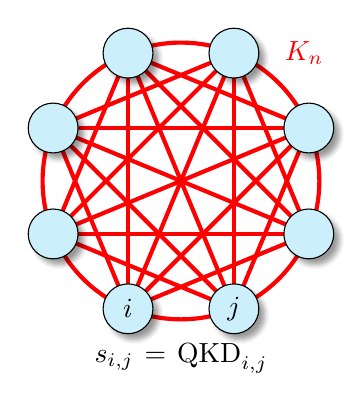
\begin{tikzpicture}[every node/.style={circle, draw, minimum size=1.8em, text width=1em, align=center, inner sep=0pt}, >=latex,
    myshadow/.style={
        blur shadow={shadow blur steps=5}
    }
]
    \def\UVsep{2.5em}
    \def\colSep{3em}
    \def\rowSep{1.2em}
    \def\hStep{0.7em}

    \definecolor{verylightgray}{rgb}{0.9, 0.9, 0.9}
    \colorlet{verylightorange}{orange!20}
    \colorlet{verylightblue}{cyan!20}

 % Radius of the circle
  \def\radius{5em}
  \def\numnodes{8}
  \def\degree{360/\numnodes}

  % Draw dummy nodes
  \foreach \x in {1,...,\numnodes} {
        \node[draw=none] (node\x) at (\x*\degree+0.5*\degree+180:\radius) {};
  }

  % Draw gray lines
  \foreach \x in {1,...,\numnodes} {
    \foreach \y in {\x,...,\numnodes} {
      \pgfmathparse{(\y>\x+1) && (1-(\x==1 && \y==\numnodes)) ? 1 : 0}
        \ifnum \pgfmathresult=1
            \draw[-,blue!20, opacity=0.5,line width=1.5,line cap=round] (node\x) -- (node\y);
        \fi
    }
  }
 \node[draw, circle, minimum size=2*\radius,blue!20, opacity=0.5,line width=1.5,line cap=round] at (0,0) {};

  % Draw red lines
  \foreach \x in {1,...,\numnodes} {
    \foreach \y in {\x,...,\numnodes} {
      \pgfmathparse{(\y>\x+1) && (1-(\x==1 && \y==\numnodes)) ? 1 : 0}
        \ifnum \pgfmathresult=1
            \draw[-,red,line width=1.5,line cap=round] (node\x) -- (node\y);
        \fi
    }
  }
 \node[draw, circle, minimum size=2*\radius,red,line width=1.5,line cap=round] at (0,0) {};

  % Visible nodes
  \foreach \x in {1,...,\numnodes} {
    \ifnum\x=1
        \node[circle,fill=verylightblue,myshadow] (node\x) at (\x*\degree+0.5*\degree+180:\radius) {$i$};
    \else
       \ifnum\x=2
            \node[circle,fill=verylightblue,myshadow] (node\x) at (\x*\degree+0.5*\degree+180:\radius) {$j$};
        \else
            \node[circle,fill=verylightblue,myshadow] (node\x) at (\x*\degree+0.5*\degree+180:\radius) {};
        \fi
    \fi
  }

  % Labels
  \coordinate (mid) at ($(node1.east)!0.5!(node2.west) + (0,-1.8em)$); 
  \node[draw=none, rectangle, text width=8em] () at (mid) {$s_{i,j}=\mathrm{QKD}_{i,j}$};
  \node[draw=none,rectangle, right=0.5em of node5,text=red] () {$K_n$};
\end{tikzpicture}
}
\hfill
\resizebox{0.49\columnwidth}{!}{
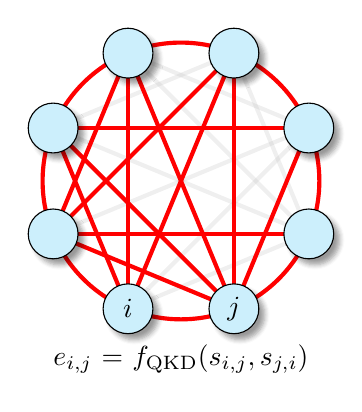
\begin{tikzpicture}[every node/.style={circle, draw, minimum size=1.8em, text width=1em, align=center, inner sep=0pt}, >=latex,
    myshadow/.style={
        blur shadow={shadow blur steps=5}
    }
]
    \def\UVsep{2.5em}
    \def\colSep{3em}
    \def\rowSep{1.2em}
    \def\hStep{0.7em}

    \definecolor{verylightgray}{rgb}{0.9, 0.9, 0.9}
    \colorlet{verylightorange}{orange!20}
    \colorlet{verylightblue}{cyan!20}

 % Radius of the circle
  \def\radius{5em}
  \def\numnodes{8}
  \def\degree{360/\numnodes}

  % Draw dummy nodes
  \foreach \x in {1,...,\numnodes} {
        \node[draw=none] (node\x) at (\x*\degree+0.5*\degree+180:\radius) {};
  }

  % Draw gray lines
  \foreach \x in {1,...,\numnodes} {
    \foreach \y in {\x,...,\numnodes} {
      \pgfmathparse{(\y>\x+1) && (1-(\x==1 && \y==\numnodes)) ? 1 : 0}
        \ifnum \pgfmathresult=1
            \draw[-,lightgray, opacity=0.25,line width=1.5,line cap=round] (node\x) -- (node\y);
        \fi
    }
  }
 \node[draw, circle, minimum size=2*\radius,lightgray, opacity=0.25,line width=1.5,line cap=round] at (0,0) {};

  % Draw red lines
  \foreach \x in {1,...,\numnodes} {
    \foreach \y in {\x,...,\numnodes} {
      \pgfmathparse{(\y>\x+1) && (1-(\x==1 && \y==\numnodes)) ? 1 : 0}
        \ifnum \pgfmathresult=1
            \pgfmathparse{(\x==1 && \y==3) || (\x==1 && \y==4) || (\x==3 && \y==5) || (\x==3 && \y==6) || (\x==3 && \y==7) || (\x==4 && \y==6) || (\x==4 && \y==8) || (\x==5 && \y==7) ? 1 : 0}
            \ifnum \pgfmathresult=0
            \draw[-,red,line width=1.5,line cap=round] (node\x) -- (node\y);
            \fi
        \fi
    }
  }
 \node[draw, circle, minimum size=2*\radius,red,line width=1.5,line cap=round] at (0,0) {};

  % Visible nodes
  \foreach \x in {1,...,\numnodes} {
    \ifnum\x=1
        \node[circle,fill=verylightblue,myshadow] (node\x) at (\x*\degree+0.5*\degree+180:\radius) {$i$};
    \else
       \ifnum\x=2
            \node[circle,fill=verylightblue,myshadow] (node\x) at (\x*\degree+0.5*\degree+180:\radius) {$j$};
        \else
            \node[circle,fill=verylightblue,myshadow] (node\x) at (\x*\degree+0.5*\degree+180:\radius) {};
        \fi
    \fi
  }

  % Labels
  \coordinate (mid) at ($(node1.east)!0.5!(node2.west) + (0,-1.8em)$); 
  \node[draw=none, rectangle, text width=10em] () at (mid) {$e_{i,j}=f_\mathrm{QKD}(s_{i,j},s_{j,i})$};
\end{tikzpicture}
}
\\
\resizebox{0.49\columnwidth}{!}{
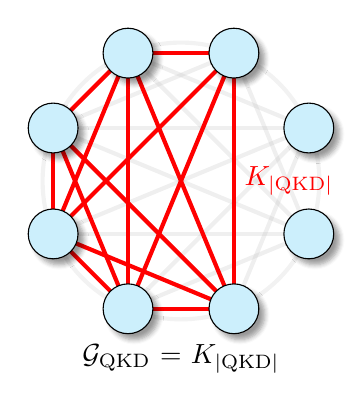
\begin{tikzpicture}[every node/.style={circle, draw, minimum size=1.8em, text width=1em, align=center, inner sep=0pt}, >=latex,
    myshadow/.style={
        blur shadow={shadow blur steps=5}
    }
]
    \def\UVsep{2.5em}
    \def\colSep{3em}
    \def\rowSep{1.2em}
    \def\hStep{0.7em}

    \definecolor{verylightgray}{rgb}{0.9, 0.9, 0.9}
    \colorlet{verylightorange}{orange!20}
    \colorlet{verylightblue}{cyan!20}

 % Radius of the circle
  \def\radius{5em}
  \def\numnodes{8}
  \def\degree{360/\numnodes}

  % Draw dummy nodes
  \foreach \x in {1,...,\numnodes} {
        \node[draw=none] (node\x) at (\x*\degree+0.5*\degree+180:\radius) {};
  }

  % Draw gray lines
  \foreach \x in {1,...,\numnodes} {
    \foreach \y in {\x,...,\numnodes} {
      \pgfmathparse{(\y>\x+1) && (1-(\x==1 && \y==\numnodes)) ? 1 : 0}
        \ifnum \pgfmathresult=1
            \draw[-,lightgray, opacity=0.25,line width=1.5,line cap=round] (node\x) -- (node\y);
        \fi
    }
  }
 \node[draw, circle, minimum size=2*\radius,verylightgray, opacity=0.5,line width=1.5,line cap=round] at (0,0) {};

  % Draw red lines
  \draw[-,red,line width=1.5,line cap=round] (node1) -- (node2);
  \draw[-,red,line width=1.5,line cap=round] (node1) -- (node5);
  \draw[-,red,line width=1.5,line cap=round] (node1) -- (node6);
  \draw[-,red,line width=1.5,line cap=round] (node1) -- (node7);
  \draw[-,red,line width=1.5,line cap=round] (node1) -- (node8);
  \draw[-,red,line width=1.5,line cap=round] (node2) -- (node5);
  \draw[-,red,line width=1.5,line cap=round] (node2) -- (node6);
  \draw[-,red,line width=1.5,line cap=round] (node2) -- (node7);
  \draw[-,red,line width=1.5,line cap=round] (node2) -- (node8);
  \draw[-,red,line width=1.5,line cap=round] (node5) -- (node6);
%  \draw[-,red,line width=1.5,line cap=round] (node5) -- (node7);
  \draw[-,red,line width=1.5,line cap=round] (node5) -- (node8);
  \draw[-,red,line width=1.5,line cap=round] (node6) -- (node7);
  \draw[-,red,line width=1.5,line cap=round] (node6) -- (node8);
  \draw[-,red,line width=1.5,line cap=round] (node7) -- (node8);

  % Visible nodes
  \foreach \x in {1,...,\numnodes} {
    \ifnum\x=1
        \node[circle,fill=verylightblue,myshadow] (node\x) at (\x*\degree+0.5*\degree+180:\radius) {};
    \else
       \ifnum\x=2
            \node[circle,fill=verylightblue,myshadow] (node\x) at (\x*\degree+0.5*\degree+180:\radius) {};
        \else
            \node[circle,fill=verylightblue,myshadow] (node\x) at (\x*\degree+0.5*\degree+180:\radius) {};
        \fi
    \fi
  }

  % Labels
  \coordinate (midK) at ($(node3)!0.5!(node4)$);
  \node[draw=none, left=0.9em of midK,text=red]
    {$K_{|\mathrm{QKD}|}$};
   
  \coordinate (mid) at ($(node1.east)!0.5!(node2.west) + (0,-1.8em)$); 
  \node[draw=none, rectangle, text width=8em] () at (mid) {$\mathcal{G}_\mathrm{QKD}=K_{|\mathrm{QKD}|}$};
\end{tikzpicture}
}
\hfill
\resizebox{0.49\columnwidth}{!}{
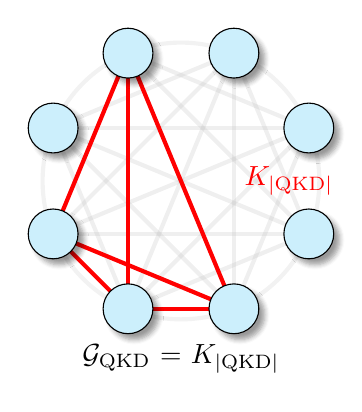
\begin{tikzpicture}[every node/.style={circle, draw, minimum size=1.8em, text width=1em, align=center, inner sep=0pt}, >=latex,
    myshadow/.style={
        blur shadow={shadow blur steps=5}
    }
]
    \def\UVsep{2.5em}
    \def\colSep{3em}
    \def\rowSep{1.2em}
    \def\hStep{0.7em}

    \definecolor{verylightgray}{rgb}{0.9, 0.9, 0.9}
    \colorlet{verylightorange}{orange!20}
    \colorlet{verylightblue}{cyan!20}

 % Radius of the circle
  \def\radius{5em}
  \def\numnodes{8}
  \def\degree{360/\numnodes}

  % Draw dummy nodes
  \foreach \x in {1,...,\numnodes} {
        \node[draw=none] (node\x) at (\x*\degree+0.5*\degree+180:\radius) {};
  }

  % Draw gray lines
  \foreach \x in {1,...,\numnodes} {
    \foreach \y in {\x,...,\numnodes} {
      \pgfmathparse{(\y>\x+1) && (1-(\x==1 && \y==\numnodes)) ? 1 : 0}
        \ifnum \pgfmathresult=1
            \draw[-,lightgray, opacity=0.25,line width=1.5,line cap=round] (node\x) -- (node\y);
        \fi
    }
  }
 \node[draw, circle, minimum size=2*\radius,verylightgray, opacity=0.5,line width=1.5,line cap=round] at (0,0) {};

  % Draw red lines
  \draw[-,red,line width=1.5,line cap=round] (node1) -- (node2);
%  \draw[-,red,line width=1.5,line cap=round] (node1) -- (node5);
  \draw[-,red,line width=1.5,line cap=round] (node1) -- (node6);
%  \draw[-,red,line width=1.5,line cap=round] (node1) -- (node7);
  \draw[-,red,line width=1.5,line cap=round] (node1) -- (node8);
%  \draw[-,red,line width=1.5,line cap=round] (node2) -- (node5);
  \draw[-,red,line width=1.5,line cap=round] (node2) -- (node6);
%  \draw[-,red,line width=1.5,line cap=round] (node2) -- (node7);
  \draw[-,red,line width=1.5,line cap=round] (node2) -- (node8);
%  \draw[-,red,line width=1.5,line cap=round] (node5) -- (node6);
%  \draw[-,red,line width=1.5,line cap=round] (node5) -- (node7);
%  \draw[-,red,line width=1.5,line cap=round] (node5) -- (node8);
%  \draw[-,red,line width=1.5,line cap=round] (node6) -- (node7);
  \draw[-,red,line width=1.5,line cap=round] (node6) -- (node8);
%  \draw[-,red,line width=1.5,line cap=round] (node7) -- (node8);

  % Visible nodes
  \foreach \x in {1,...,\numnodes} {
    \ifnum\x=1
        \node[circle,fill=verylightblue,myshadow] (node\x) at (\x*\degree+0.5*\degree+180:\radius) {};
    \else
       \ifnum\x=2
            \node[circle,fill=verylightblue,myshadow] (node\x) at (\x*\degree+0.5*\degree+180:\radius) {};
        \else
            \node[circle,fill=verylightblue,myshadow] (node\x) at (\x*\degree+0.5*\degree+180:\radius) {};
        \fi
    \fi
  }

  % Labels
  \coordinate (midK) at ($(node3)!0.5!(node4)$);
  \node[draw=none, left=0.9em of midK,text=red]
    {$K_{|\mathrm{QKD}|}$};
   
  \coordinate (mid) at ($(node1.east)!0.5!(node2.west) + (0,-1.8em)$); 
  \node[draw=none, rectangle, text width=8em] () at (mid) {$\mathcal{G}_\mathrm{QKD}=K_{|\mathrm{QKD}|}$};
\end{tikzpicture}
}
%	\includegraphics[width=\columnwidth]{figures/proof_chains_QKD.pdf}	
	\caption{\textbf{QKD proof-chain for shared quantum randomness.} Amongst $n$ nodes with full $O(n^2)$ quantum communications connectivity given by the complete graph $K_n$, every node executes a QKD protocol with every other node, associating a shared random bit-string $s_{i,j}$ (received by $i$ from $j$) with every edge. Bit-strings passing a QRN certification function $f_\mathrm{QKD}(s_{i,j},s_{j,i})$ define the edges of a subgraph, where certification acts as an implied vote of honesty. Maintaining only vertices connected to a majority of other nodes followed by eliminating those not connected to every other, we obtain a complete subgraph $\mathcal{G}_\mathrm{QKD}$ reflecting the unanimous majority.} \label{fig:proof_chains_QKD}
\end{figure}

\subsubsection{Consensus protocol}

Associating QKD bit-strings $s_{i,j}$ with graph edges we assume a certification function,
\begin{align} \label{eq:QKD_verif}
	f_\mathrm{QKD}(s_{i,j},s_{j,i})\to \{0,1\},
\end{align}
which evaluates \texttt{true} if $s_{i,j}$ passes a certification test for randomness. We define a QKD compliance graph with edge-inclusion based on the validity of the respective QKD bit-strings,
\begin{align}
	\mathcal{G}_\mathrm{QKD}^{(\mathrm{comp})}: e_{i,j} = f_\mathrm{QKD}(s_{i,j}).
\end{align}
Letting the QKD compliance of nodes be,
\begin{align} \label{eq:QKD_node_comp}
	\mathcal{G}_\mathrm{QKD}^{(\mathrm{comp})}: v_i = \textsc{Majority}\left(\bigcup_{j\neq i} e_{i,j}\right),
\end{align}
the reduced graph now only contains nodes whose associated QKD bit-strings $s_{i,j}$ are majority valid.

Additionally requiring unanimity demands finding a fully-connected subgraph, or clique\footnote{While the \textsc{MaxClique} problem of finding the largest cliques in a graph is known to be \textbf{NP}-complete in general, here we are not finding maximal cliques, affording an efficient solution.}, achieved by eliminating all vertices in $\mathcal{G}_\mathrm{QKD}^{\mathrm{(comp)}}$ not connected by an edge to every other node,
\begin{align}
	\mathcal{G}_\mathrm{QKD}: v_i =
    \begin{cases}
        1 & \text{if } |u_i \in \mathcal{G}_\mathrm{QKD}^{\mathrm{(comp)}}| = |\mathcal{G}_\mathrm{QKD}^{\mathrm{(comp)}}| - 1\\
        0 & \text{otherwise}
    \end{cases}.
\end{align}
The fully connected \mbox{$\mathcal{G}_\mathrm{QKD}= K_{|\mathcal{G}_\mathrm{QKD}|}$} subgraph now represents the accepted subset of QKD-compliant nodes under consensus. The associated collectively established shared random bit-string is defined as,
\begin{align}
	s(\mathcal{G}_\mathrm{QKD}) = \bigoplus_{v_i,v_j\in \mathcal{G}_\mathrm{QKD}} {s_{i,j}}.
\end{align}

Although nodes could commit post-processed QKD strings obtained following post-selection and privacy amplification, this requires interaction between respective nodes. In the interests of maintaining a broadcast-only communications interface nodes may simply commit their raw unprocessed strings ($b$ and $m$) from which the associated QRNs $s$ are implied under a network-agreed post-processing function $f_\mathrm{PP}(\vec{b},\vec{m})\to \vec{s}$. 

\subsection{Interactive proofs of quantumness} \label{sec:IPQ}

%\begin{figure}[!htb]
%	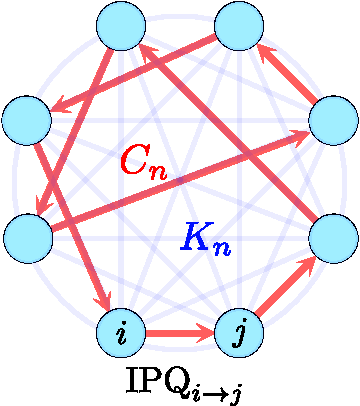
\includegraphics[width=0.35\columnwidth]{figures/proof_chains_IPQ.pdf}	
%	\caption{Proof-chain for shared quantum randomness. Amongst $n$ nodes with full quantum communications connectivity given by the complete graph $K_n$, nodes are randomly assigned to a cyclic graph $C_n\subseteq K_n$. Edges $e_{i,j}$ represent the establishment of shared quantum-random bit-strings between nodes. For entanglement-based (E91) randomness edges are undirected as the protocol is symmetric between $i$ and $j$. For BB84- and prover/verifier-based protocols nodes roles are asymmetric and edges are directed.} \label{fig:proof_chains_IPQ}
%\end{figure}

%Requiring all nodes to act as both prover and verifier once implies all vertices have in-degree and out-degree of 1,
%\begin{align}
%	\mathrm{deg}(v) = \mathrm{deg}(v) = 1\,\,\forall\,v\in V.
%\end{align}
%This implies the prover-verifier graph is a sum of disjoint cyclic graphs spanning all all nodes $v\in V$,
%\begin{align}
%	G_n = \sum_{\sum_i n_i = n} C_{n_i}	
%\end{align}

%If $G_n$ is the directed verifier graph the converse graph $G_n^\top$ represents the prover graph.
%
%Shared quantum-randomness requires only that a single QKD exchange be honest. i.e a single prover must be engaged honestly.

An interactive proof of quantumness \cite{Liu22, Zhu23} comprises two parties, a \emph{prover} and a \emph{verifier}, where the goal is for the prover to prove to the verifier that they have honestly executed a quantum implementation of some function $f(\cdot)$ that cannot be spoofed by classical simulation. The verifier has only classical resources and both parties may classically communicate.

While such protocols are not known in general for arbitrary $f(\cdot)$, they have been described in the context of a restricted class of functions known as trapdoor claw-free functions.

\subsubsection{Trapdoor claw-free (TCF) functions}

Trapdoor claw-free functions (TCF) are a class of cryptographic, 2-to-1, one-way functions,
\begin{align}
	f_\mathcal{I}(x)\to w,
\end{align}
which are classically efficient to evaluate in the forward direction, but for which it is hard to find simultaneously satisfying inputs $\{x_0,x_1\}$ (the `claw') mapping to the same output,
\begin{align}
	f(x_0)=f(x_1)=w,
\end{align}
where $x\in \{0,1\}^n$ and $w\in\{0,1\}^{n-1}$ are bit-strings.

Here, $\mathcal{I}$ denotes a problem instance derived from a secret (the trapdoor). If the secret is known, finding claws $\{x_0,x_1\}$ is classically efficient for any $w$. Since $f(\cdot)$ is easy to evaluate in the forward direction, verifying solutions is classically efficient, and the problem of  claw-finding by definition resides in the complexity class \textbf{NP}. %However, since inverting the trapdoor is hard the problem lies outside of the complexity class \textbf{P}, and outside \textbf{BQP} for post-quantum trapdoor functions.

%For an interactive proof of quantumness we desire claw-finding to be post-quantum and reside outside \textbf{BQP} such that a quantum prover is unable to spoof solutions by compromising the cryptographic integrity of $f(\cdot)$.

\subsubsection{The LWE problem}

A candidate TCF is the lattice-based learning with errors (LWE) problem \cite{Goldwasser85, Regev09, Regev10}. This problem is believed to be post-quantum, where the associated claw-finding problem lies outside of \textbf{BQP}, the class of problems efficiently solvable by quantum computers\footnote{An alternate number-theoretic TCF based on Rabin's function has been described \cite{Rabin79, Goldwasser88}. Since here the complexity of inverting the trapdoor reduces to integer factorisation this candidate TCF is vulnerable to quantum attack via Shor's algorithm \cite{Shor97}, making it less applicable in the assumed context of universal quantum computation.}.

For matrix,
\begin{align}
	A\in\mathbb{Z}_q^{m\times n},
\end{align}
and vectors,
\begin{align}
	x,y,s,e\in\{0,1\}^n,
\end{align}
related by,
\begin{align}
	y = A\cdot s + e,
\end{align}
under modulo $q$ arithmetic where $q$ is prime, a TCF may be constructed as,
\begin{align}
	f_\mathcal{I}(b,x_b) &= \lfloor A\cdot x + b\cdot y\rceil,
\end{align}
where $b=\{0,1\}$ is a single bit and claws are related by,
\begin{align}
	x_0=x_1+s.
\end{align}
Here, $\mathcal{I}=\{A,y\}$ specifies the problem instance derived from the secret trapdoor $\mathcal{T}=\{s,e\}$ secretly held by the verifier, enabling efficient classical claw-finding and verification if known.

Since $f(x)\to w$ is classically efficient to evaluate in the forward direction, it is easy to find a $w$ for which a single satisfying input $x$ is known. The challenge lies in finding simultaneously satisfying pairs of inputs, believed to be hard for both classical and quantum computers.

\subsubsection{Interactive proof protocol}

Taking a cryptographic TCF function, $f_\mathcal{I}(x)\to w$, an interactive proof of quantumness may be implemented as follows:

\begin{enumerate}
	\item The verifier specifies a problem instance $\mathcal{I}$, without revealing the associated secret $\mathcal{T}$ from which it was derived.
	\item The prover prepares a uniform superposition of all length-$n$ bit-strings $x$ via a Hadamard transform,
\begin{align}
	\ket{\psi_H} &= \hat{H}^{\otimes n} \ket{0}^{\otimes n} = \frac{1}{\sqrt{2^n}} \sum_{x\in\{0,1\}^n} \ket{x}.
\end{align}
	\item Evaluating $f_\mathcal{I}(x)$ into an output register yields\footnote{The unitarity of quantum circuits prohibits direct evaluation of classical functions on quantum registers in general,
	\begin{align}
		\hat{U}_f\ket{x}\not\to\ket{f(x)},\nonumber
	\end{align}
	where $\hat{U}_f$ denotes a quantum circuit evaluating classical function $f(\cdot)$. Introducing ancillary quantum register $\ket{y}$, evaluation of,
	\begin{align}
		\hat{U}_f\ket{x}\ket{y}\to\ket{x}\ket{y\oplus f(x)},\nonumber
	\end{align}
	may be implemented unitarily in general. Considering a single output bit of $f(\cdot)$, $\hat{U}_f$ admits the decomposition,
	\begin{align}
		\hat{U}_f = \hat\Pi_0\otimes \hat{I} + \hat\Pi_1\otimes \hat{X},\nonumber
		\end{align}
	where,
	\begin{align}
		\hat\Pi_i = \sum_{x\,|\,f(x)=i}\ket{x}\bra{x},\nonumber
	\end{align}
	are projectors onto the subspaces of $x$ satisfying \mbox{$f(x)=i$} (Nb: \mbox{$\hat\Pi_0+\hat\Pi_1=\hat{I}$}, \mbox{$\hat\Pi_0\cdot\hat\Pi_1=0$}). The unitarity of $\hat{U}_f$ follows, independent of $f(\cdot)$,
	\begin{align}
		\hat{U}_f^\dag \cdot \hat{U}_f &= (\hat\Pi_{0}\otimes \hat{I} + \hat\Pi_1\otimes \hat{X})^2 = \hat{I}.\nonumber
	\end{align}
	Repeating for all output bits and letting \mbox{$y=0$} yields,
	\begin{align}
		\hat{U}_f\ket{x}\ket{0}\to\ket{x}\ket{f(x)}.\nonumber
	\end{align}},
	\begin{align}
		\ket{\psi_\mathcal{I}} &= \frac{1}{\sqrt{2^n}} \sum_{x\in\{0,1\}^n} \ket{x} \ket{f_\mathcal{I}(x)},\nonumber
	\end{align}
	which may be efficiently prepared using a quantum circuit with,
	\begin{align}
		O(n^2 \log^2 n),
	\end{align}
	gate count \cite{ClassVerifQA}.
	\item The prover measures the output register, obtaining measurement outcome $w$ which is communicated to the verifier. Measuring $w$ collapses the $x$-register onto the equal superposition of associated satisfying pre-images,
\begin{align}
	\ket{\psi_w} = \frac{1}{\sqrt{2}}(\ket{x_0}+\ket{x_1})\ket{w}.
\end{align}
As the $x$-register was initialised into a uniform superposition over all length-$n$ bit-strings and the TCF is a 2-to-1 function, $w$ is sampled uniformly at random.
	\item The verifier specifies a random measurement basis in which the prover should measure qubits in the $x$ register, where $b=\{0\equiv \hat{Z},1\equiv\hat{X} \}$ correspond to the respective Pauli measurement bases.
	\item When measuring in the $b=0$ ($\hat{Z}$) basis, the prover randomly measures either $m=x_0$ or $m=x_1$, easily verified by direct evaluation of \mbox{$f(x)\to w$} and comparison with the prover's previously reported $w$. When measuring in the $b=1$ ($\hat{X}$) basis verification succeeds if \mbox{$m\cdot x_0 = m\cdot x_1$}. The verification rules are,
\begin{align}
 	\hat{Z}\, (b=0):&\quad m=\{x_0,x_1\},\nonumber\\
	\hat{X}\, (b=1):&\quad m\cdot x_0 = m\cdot x_1.
\end{align}
	\item The above is repeated some constant number of rounds, independently randomising the measurement basis $b$ at every round.
\end{enumerate}

The key observation is that since $\hat{X}$ and $\hat{Z}$ measurements do not commute, it is not possible for the prover to know both measurement outcomes simultaneously and therefore must measure in accordance with the verifier's stated measurement basis to pass verification of a single round. While a single round can be classically spoofed if the measurement basis $b$ is known in advance of announcing $w$, if unknown, $b$ can only be guessed with a probability of $1/2$. Upon repetition, the probability of correctly guessing all measurement bases scales as \mbox{$p=1/2^n$} for $n$ rounds, ensuring asymptotic confidence in the honesty of the prover.

\subsubsection{Consensus protocol}

To incorporate IPQs into the QCN framework we require all nodes to act as both prover and verifier for all other nodes.

In the verifier capacity every node prepares a single random TCF instance for all other nodes to prove. Despite solving the same problem instance their proofs will be distinct.

Following the same approach as with QKD we represent the proofs-of-quantumness via a complete graph with the distinction that as this is an asymmetric protocol the graph is now directed (from prover to verifier) with edges in both directions for every node-pair.

Majority votes as per Eq.~\eqref{eq:QKD_node_comp} are now made from the verifier perspective.

The additional synchronous steps required to accommodate IPQs are:
\begin{enumerate}
	\item Nodes commit a single random problem instance $\mathcal{I}_i$.
	\item Nodes execute the quantum problem instance specified by every other node $j$ and commit the obtained $w_{i,j}$.
	\item Nodes commit the random measurement bases $b_i$ other nodes will be required to measure in.
	\item Nodes complete their quantum computations and commit the obtained measurements $m_{i,j}$.
	\item Nodes reveal their secrets $\mathcal{T}_i$.
\end{enumerate}
	
Assuming a verification function analogous to Eq.~\eqref{eq:QKD_verif},
\begin{align}
	f_\mathrm{IPQ}(\mathcal{I}_i,\mathcal{T}_i,w_{i,j},b_i,m_{i,j}) \to \{0,1\},
\end{align}
similarly defines a directed IPQ compliance graph,
\begin{align}
	G_\mathrm{IPQ}^{\mathrm{comp}}: e_{i,j} = f_\mathrm{IPQ}(\mathcal{I}_i,\mathcal{T}_i,w_{i,j},b_i,m_{i,j}) \to \{0,1\}.
\end{align}
	
%A classical cheater can spoof a single round of this protocol if the measurement basis is known in advance. For example, if known that the measurement basis will be $Z$, they can choose a random $x$, efficiently evaluate $f(x)\to w$ in the forward direction, and pass the $Z$ test. However, if $b$ is chosen at random, they will only be able to do this half the time if the full claw is not known. 

%
%The full proof for a multi-round implementation of this protocol between provers ($i\in\mathcal{S}_P$) and verifiers ($j\in\mathcal{S}_V$) is given by,
%\begin{align}
%	\mathcal{P}_{i,j} = \{\mathcal{I}_j,\{w_{i,j}^{(k)}\},\{b_{j}^{(k)}\},\{m_{i,j}^{(k)}\}\},
%\end{align}
%where $0\leq k < N_R$ indexes the round.

%\section{QIP}
%
%From the proof system, $\mathcal{P}_S$, we define the node keys,
%\begin{align}
%	k_i &= \bigoplus_{j,k} w_{i,j}^{(k)},
%\end{align}
%for each prover $i\in\mathcal{S}_P$, and a collective key,
%\begin{align}
%	k &= \bigoplus_i k_i,
%\end{align}
%which is guaranteed to be quantum-random if at least one proof was honest and obtained via quantum computation. Under the action of the bitwise XOR operation on the set $\{k_i\}$, $k$ implements a random permutation $\sigma\in S_{|\mathcal{S}_P|}$ on the ordering of the set of provers $\mathcal{S}_P$ ,
%\begin{align}
%k \oplus \{k_i\} \cong \sigma(\mathcal{S}_P),
%\end{align}
%where $\sigma\in S_{|\mathcal{S}_P|}$ denotes a permutation in the symmetric group over $|\mathcal{S}_P|$ elements.
%
%Exploiting this property, for each prover we define the permuted key,
%\begin{align}
%	\tilde{k}_i &= k \oplus k_i	= \bigoplus_{j\neq i} k_j,
%\end{align}
%which cannot be manipulated as $k$ is not known prior to commitment of $\{k_i\}$.
%
%Ordering provers by $\tilde{k}_i$ creates a quantum randomly ordered set. Upon piecewise partitioning we obtain non-intersecting random subsets, all perfect quantum-random solutions to the random subset problem, assuming at least one honest proof.

\section{Economics} \label{sec:economics}

Internally, the DCN operates as a cooperative, profit-neutral, barter economy, whose nodes facilitate an externally-facing competitive bidding market for consensus. Nodes' subjective cost of consensus is identically their own computational execution cost, individually incentivising computational and communications implementation efficiency.

Proof-of-work associates the creation of money with exchange, creating a monetary dependence on algorithmic inefficiency. DCNs are monetarily neutral, providing consensus as a generic and abstract commodity in a competitive market environment.

The DCN is a floating market instrument with instantaneous value. Consensus is necessarily consumed upon production and cannot be saved.

%In a competitive market the cost of consensus approximates its production cost.

%A market of freedom and equality.

%While consensus is a tradable commodity with market value, a DCN network is able to operate without 

%During the \textsc{Bid} stage of the protocol, bids presented to the network demand $N_C$ units of work to undergo consensus, 1 unit of work per honest consensus participant. 

%The set of PoCs produced during a round of the protocol collectively reveal the compliance of all network nodes. Nodes contribute 1 unit of work to the network for every consensus they faithfully execute, and consume $N_C$ units of work for every submitted \texttt{statement} subject to consensus.

%During the \textsc{Accept} stage all network nodes are additionally required to agree upon the network's ledger state, where compliant nodes from the previous round have their workload tallies incremented by consensus' they faithfully contributed to and decremented by the the workload consumed by \texttt{statements} they submit for consensus.

%* Upon bidding to participate, nodes promise to faithfully participate in consensus via a deposit. During the \textsc{Accept} stage, this requires nodes' work tallies to be at least as large as their promise. The subsequent ledger state deducts promises from the tallies of non-compliant nodes. To incentivise compliance, the required promise amount must exceed the objective cost of execution.

%This policy enforces neutrality between nodes' contributed and consumed consensus load. While compliance ensures the ledger is monetarily neutral, non-compliance results in the destruction of credits via the associated unreturned deposits, and nodes with insufficient credits from a history of non-compliance are unable make promises for future participation and barred from participation. Here network policy must stipulate buy-in mechanisms for the creation of new consensus credits, for example by settling against external ledgers.

%* Supply side highly competitive. Demand side for access to the network, a floating market entity.

%* Economics based on contribution rather than waste.

%* The network’s economy involves only the direct and simultaneous steady-state exchange of contribution towards consensus — monetarily neutral with no dependence on external currency, driven  only by demand for consensus.

%* New nodes buy into the network by pre-contributing sufficient work to afford future payment for consensus. Accumulated credits by contributing more than is requested additionally acts as a buffer against unintended non-compliance, for example as a result of communications failure. If service distraction prevents participation in consensus the buffer ensures the ability to maintain requests. monetarily neutral.

%* Participation in consensus is a mutual exchange of randomness. The economy of the DCN is driven only by its demand.

%* An open ecosystem driven by mutual exchange, equity and consent.

Consensus nodes individually utilise and monetise their gateway to the network facilitating highly competitive and high volume consensus markets.

\section{Applications} \label{sec:applications}

\subsection{Protocols}

Protocols are user-level applications for consensus, defined as arbitrary time-dependent functions acting on the current state of the broadcast channel,
\begin{align}
	\textsc{Protocol}(\mathcal{B}(t=0),\star)\to \star,
\end{align}
where time is relative to the present. The state of the broadcast channel a time $t$ contains all previous messages broadcasts,
 where,
\begin{align}
	\mathcal{B}(t=0) = \bigcup_{x\in \mathcal{B}(t\leq 0)} x.
\end{align}

The state of the broadcast channel is in general subjective as individual users may have imperfect knowledge of $\mathcal{B}$ as a result of information loss. The subjective state of the broadcast channel for user $i$ is,
\begin{align}
	\mathcal{B}_i \subseteq \mathcal{B}.
\end{align}
Consequently, \textsc{Protocol} outputs are also subjective and may differ in general,
\begin{align}
	\textsc{Protocol}_i(\mathcal{B}_i,\star) \neq \textsc{Protocol}(\mathcal{B},\star)
\end{align}

\subsection{Ledgers}

Consensus is formed on state register transformations.

Ledgers are defined by policies stipulating the consensus networks they recognise. Inter-ledger operations require only mutual recognition of consensus networks.

Ledgers as oracles.

Finite state machine oracles.

The combined public broadcasts across all networks acts as a global oracle for ledger states, facilitating a high arbitrage environment in an algorithmic context, an equilibrating force across the ledgers of parallel markets or interconnected markets.

Inter-ledger transactions require only mutual recognition of consensus, defined by the networks from which they are drawn.

* Sec: ledger transaction queues.

* Hierarchical bidding to maximise resource utilisation.

\subsection{Blockchains}

Blockchains are protocol-level applications for consensus, following their own rules on what consensus is formed on. A blockchain's transaction history is immutable and may be retrospectively evaluated. Blockchain implementations typically consider asynchronous operating environments. In this setting simultaneous block additions manifest themselves as forks, requiring error correction mechanisms to maintain the integrity of the chain. Formally, a pool of valid block additions defines a directed tree graph which the blockchain implementation must correct to a directed linear graph.

In a synchronous setting where a ledger is associated with consensus derived from a given network these considerations change. Rather than performing consensus assignment on the basis of unique transaction identifiers we assign on the basis of transaction queue identifiers associated with individual ledgers. From the pool of accepted bids nodes assigned to a given transaction queue consensus set process all bids associated with that queue, batch processed in accordance with the ledger's transaction amalgamation rules. Employing queue assignment rather than transaction assignment mitigates the possibility of fork formation. In a proof-of-work setting this issue may be addressed by introducing friction. However, while this hinders double-mining it also undermines transaction processing rates, an undesirable tradeoff.

If $n$ consensus sets of size $N$ independently form honest majority their union of size $nN$ necessarily forms honest majority. Hence,
\begin{align}
	P(nN,r)\leq\varepsilon \,\Rightarrow\, P(N,r)^n\leq\varepsilon.
\end{align}
For $n=1$ this reduces to consensus by majority vote amongst $N$ parties, while the opposing limiting case of $n=N$ reduces to consensus by unanimity amongst $N$ parties. A blockchain with unanimous $n$-level retrospective verification affords $\varepsilon^n$-security, and the associated tradeoff in required consensus set size scales as,
\begin{align}
	N_\mathrm{min}(r,\varepsilon) = N_\mathrm{min}^{(n)}(r,\varepsilon^n),
\end{align}
which implies,
\begin{align}
	P_c(N,r) = P_c(N^{(n)},r)^n.
\end{align}

Now $\varepsilon$ represents the effective error rate in new block additions while \mbox{$\varepsilon'=\varepsilon^n$} is the effective security parameter which applies only to blocks at least $n$ steps back, which have been subject to $n$ independent verifications. These blocks are considered \emph{complete} whereas more recent blocks are considered \emph{pending}, potentially still subject to being invalidated (Fig.~\ref{fig:backward_integrity}). Only the most recent \emph{complete} block must persist to maintain the blockchain, the point to which the blockchain is reverted if \emph{pending} blocks are invalidated.

\begin{figure}[!htb]
\begin{tikzpicture}[genericStyle, scale=0.5]
  \def\myWidth{6em}
  \def\myHeight{2.5em}

  \fill[fill=topologyFillColor] (-\myWidth,0) rectangle (\myWidth,10.5);

  \node[draw=none, fill=cyan!20, ellipse, minimum width=\myWidth, minimum height=\myHeight, fill=blockchainDiscColor, myShadow] (node0) at (0,0) {$\varepsilon^n$};
  \node[draw=none, ellipse, minimum width=\myWidth, minimum height=\myHeight, fill=blockchainDiscColor] (node1) at (0,3.5) {$\varepsilon^n$};
  \draw[darkgray] (-\myWidth,3.5) arc [start angle=0, end angle=-180, x radius=-\myWidth, y radius =\myHeight];
  \draw[gray, dashed] (-\myWidth,3.5) arc [start angle=0, end angle=180, x radius=-\myWidth, y radius =\myHeight];

  \node[draw=none, ellipse, minimum width=\myWidth, minimum height=\myHeight, fill=blockchainPendingDiscColor] (node2) at (0,5) {$\varepsilon^n$};
  \draw[darkgray] (-\myWidth,5) arc [start angle=0, end angle=-180, x radius=-\myWidth, y radius =\myHeight];
  \draw[gray, dashed] (-\myWidth,5) arc [start angle=0, end angle=180, x radius=-\myWidth, y radius =\myHeight];

  \node[draw=none, ellipse, minimum width=\myWidth, minimum height=\myHeight, fill=blockchainPendingDiscColor] (node3) at (0,7) {$\varepsilon^{n-1}$};
  \draw[darkgray] (-\myWidth,7) arc [start angle=0, end angle=-180, x radius=-\myWidth, y radius =\myHeight];
  \draw[gray, dashed] (-\myWidth,7) arc [start angle=0, end angle=180, x radius=-\myWidth, y radius =\myHeight];

  \draw[darkgray] (-\myWidth,0) arc [start angle=0, end angle=-180, x radius=-\myWidth, y radius =\myHeight];
  \draw[gray, dashed] (-\myWidth,0) arc [start angle=0, end angle=180, x radius=-\myWidth, y radius =\myHeight];

  \node[draw=none] (node4) at (0,2) {$\vdots$};
  \node[draw=none] (node4) at (0,9) {$\vdots$};
  \node[darkgray, ellipse, minimum width=\myWidth, minimum height=\myHeight, fill=blockchainPendingDiscColor] (node5) at (0,10.5) {$\varepsilon$};

  \draw (-\myWidth,0) -- (-\myWidth,10.5);
  \draw (\myWidth,0) -- (\myWidth,10.5);

  \coordinate (ltop) at ($(node5.west) + (-2em,0)$);
  \coordinate (lbot) at ($(node2.west) + (-2em,0)$);
  \coordinate (backC) at ($(ltop.west)!0.5!(lbot.west) + (-1.2em,0)$);

  \coordinate (pendtop) at ($(node5.east) + (2em,\myHeight)$);
  \coordinate (pendbot) at ($(node2.east) + (2em,0)$);
  \coordinate (pendtopin) at ($(pendtop) + (-0.5em,0)$);
  \coordinate (pendbotin) at ($(pendbot) + (-0.5em,0)$);
  \coordinate (pendC) at ($(pendbot)!0.5!(pendtop) + (1.5em,0)$);

  \coordinate (comptop) at ($(node1.east) + (2em,\myHeight)$);
  \coordinate (compbot) at ($(node0.east) + (2em,-\myHeight)$);
  \coordinate (comptopin) at ($(comptop) + (-0.5em,0)$);
  \coordinate (compC) at ($(compbot)!0.5!(comptop) + (1.5em,0)$);

  \draw[darkgray, <->, thick] (ltop) -- (lbot);
  \draw[redHighlightColor, thick] (pendtopin) -- (pendtop) -- (pendbot) -- (pendbotin);
  \draw[->, blueHighlightColor, thick] (comptopin) -- (comptop) -- (compbot);

  \node[draw=none, rotate=90, text=red] at (pendC) {pending};
  \node[draw=none, rotate=90, text=blue] at (compC) {complete};
  \node[draw=none, text=black] at (backC) {$n$};
\end{tikzpicture}
%\includegraphics[width=0.5\columnwidth]{figures/backward_integrity.pdf}
\caption{\textbf{Blockchain with $n$-level reverse integrity checking.} Upon addition of the top-level block consensus requires verifying integrity going back $n$ blocks. If consensus has $\varepsilon$-security, for $i\leq n$ the $i$th past block will have been verified $i$ times, exhibiting cumulative $\varepsilon^i$-security. Blocks $i\geq n$ all exhibit $\varepsilon'=\varepsilon^n$ integrity, the security parameter of the blockchain. The $\varepsilon$-security of the top block may be interpreted as the effective error rate in block addition, where error correction is implemented at the blockchain's protocol level.} \label{fig:backward_integrity}
\end{figure}

\begin{figure}[!htb]
\centering
\resizebox{\columnwidth}{!}{
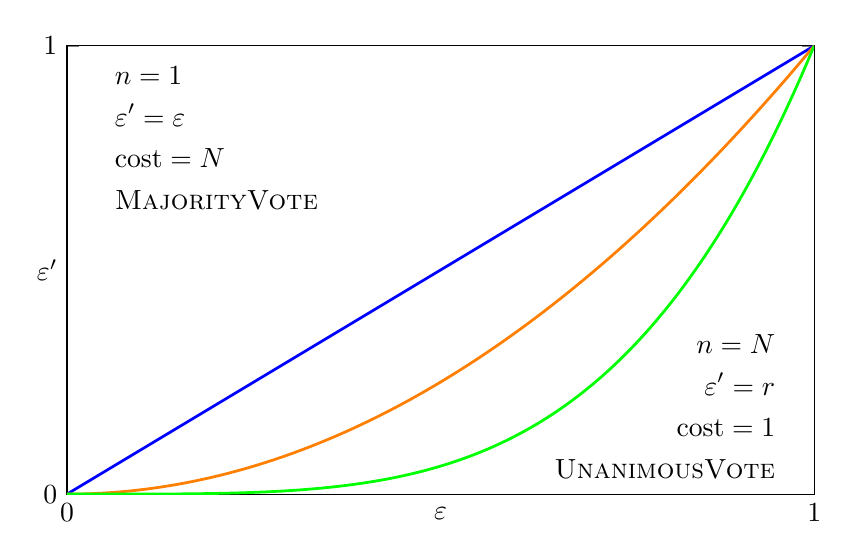
\begin{tikzpicture}
\begin{axis}[
    xlabel={$\varepsilon$},
    ylabel={$\varepsilon'$},
    xmin=0, xmax=1,
    ymin=0, ymax=1,
    restrict y to domain=0:1,
    grid style=dashed,
    xtick={0, 1},
    ytick={0, 1}, 
    ylabel style={rotate=-90, xshift=1.2em},
    xlabel style={yshift=1.2em},
    unit vector ratio=5 3,
]

% Plot x
\addplot[
    color=blue,
    domain=0:1,
    samples=200,
    line width=1pt,
    ]
    {x};

% Plot x^2
\addplot[
    color=orange,
    domain=0:1,
    samples=200,
    line width=1pt,
    ]
    {x^2};

% Plot x^3
\addplot[
    color=green,
    domain=0:1,
    samples=200,
    line width=1pt,
    ]
    {x^4};
% \addlegendentry{$x^4$}

\node at (axis cs:0.2,0.8) {\parbox{4cm}{
        \begin{align*}
            &n = 1\\
            &\varepsilon'=\varepsilon\\
            &\mathrm{cost}=N\\
            &\textsc{MajorityVote}
        \end{align*}
    }};

\node at (axis cs:0.8,0.2) {\parbox{4cm}{
        \begin{align*}
            n = N\\
            \varepsilon'=r\\
            \mathrm{cost}=1\\
            \textsc{UnanimousVote}
        \end{align*}
    }};


\end{axis}
\end{tikzpicture}
}
%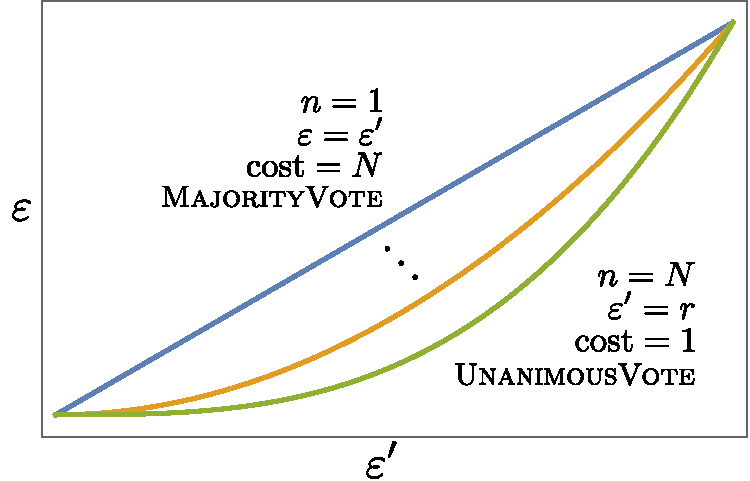
\includegraphics[width=\columnwidth]{figures/blockchain_security_tradeoffs.pdf}
\caption{\textbf{Tradeoffs in blockchain integrity with retrospective consensus verification.}}\label{fig:blockchain_security_tradeoff}	
\end{figure}

\subsection{Distributed computing}

The consensus assignment problem may be interpreted more generically as randomised dynamic load allocation.

Consider the case of $|\mathcal{C}|=1$ consensus sets, the delegation of computational workloads to single randomly allocated nodes. In this context the consensus assignment algorithm facilitates dynamic load balancing across the network. Similarly, \mbox{$|\mathcal{C}|>1$} equates to dynamic allocation with $|\mathcal{C}|$-fold redundancy where consensus is formed on the outcome.

More generally, \textsc{MapReduce}-type  \cite{MapReduce} computations may be delegated to consensus sets of arbitrary size, where the \textsc{Map} routine corresponds to the assignment of consensus nodes and the \textsc{Reduce} routine is evaluated by consensus.

* Distributed queries.

* Consider asymmetric bidding if preserving $r$ is not a consideration.

\subsection{Distributed signature authorities}

* Consensus on state of knowledge. Trust in knowledge. Oracle.

%\section{Resource consumption}

%Distributed consensus networks are highly resource-efficient, as all nodes participate in consensus, and the allocation of consensus sets is.

\section{Strategic considerations} \label{sec:strategic_cons}

??? TO DO

\begin{figure}[!htb]
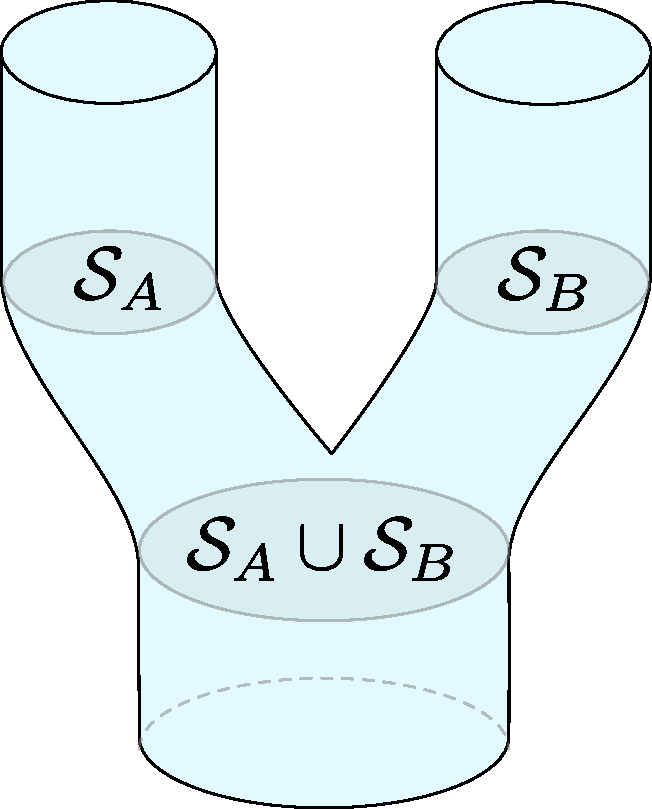
\includegraphics[width=0.7\columnwidth]{figures/forking.pdf}
\caption{\textbf{Bifurcation in network trust.} When the network $\mathcal{S}_A\cup\mathcal{S}_B$ supporting a blockchain segregates into two non-interacting networks, $\mathcal{S}_A$ and $\mathcal{S}_B$, a fork is created, forming two unique, legitimate blockchains, one associated with each network.} \label{fig:forking}	
\end{figure}

\begin{figure}[!htb]
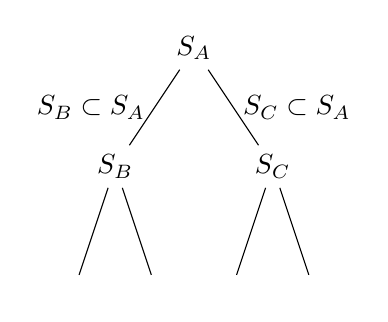
\begin{tikzpicture}
 [level distance=15mm,level/.style={sibling distance=20mm/#1}]
  \node {$S_A$}
    child {node {$S_B$}
      child {node {}}
      child {node {}}
      edge from parent node[left,draw=none] {$S_B\subset S_A$}
    }
    child {node {$S_C$}
      child {node {}}
      child {node {}}
      edge from parent node[right,draw=none] {$S_C\subset S_A$}
    };
\end{tikzpicture}
\caption{Trust hierarchies represented as subset-trees define retreat strategies.} \label{fig:subset_tree}
\end{figure}

Fig.~\ref{fig:subset_tree}

`Rebasing' network upon strategic retreat.

Retreat strategy in trust hierarchy where root is level $i=0$. Levels represent set containment, $s_{i+1}\subset s_i$. Retreat to smallest i (i.e largest trusted subset). Assume that $r_{i+1}<r_i$. Inequality could work in either direction??

\section{Conclusion} \label{sec:conclusion}

%Contrary to existing blockchain design philosophy, the abstract separation between digital assets and their technological mechanism for trade provides a framework under which both may compete in a competitive market environment, enabling the emergence of a free banking system.
%
%DCNs are generically applicable, automated digital signature systems and neither inherently transactional nor monetary in nature, reducing exposure to escalating regulatory efforts to restrict the trade of digital assets and inhibit technological innovation \cite{DAAMLA}.

\begin{acknowledgments}
%I thank \href{https://youtube.com/playlist?list=PLeRYUHyTyGxaeZpLq_YxA2D4Ydiq7QfHg}{Aiguilles d'Entr{\`e}ves} for the inspiration that led to this work.
\end{acknowledgments}

\bibliography{bibliography}

\end{document}

\section{Miscellaneous notes}

Upon post-selection the accepted set of participants are in unanimous agreement on set membership.
Attestations for accepted participants.

Although PoCs execute in synchronous environments they are asynchronous objects.

Nodes evaluate time-compliance based on time-of-receipt, enforcing an effective lower-bound on delta. All time-of-receipts (sender excluded) are commit-revealed. Consensus-time at each synchronous step of the protocol is with respect to the time-of-receipts of messages associated with the respective protocol stage: acceptance, consensus and compliance.

Dynamic networks: Dynamic network membership: network algorithmically implements policies on network’s nodes and parameters. Could be democratic.

Proof-of-work artificially ties monetary dynamics with its gross inefficiency, where transaction cost …

Nodes' time accuracy is economically self-incentivised towards accuracy.

Deferred proof-of-consensus: provide only proof of random subsets but not consensus, which can be made at a later point.

Node announcements are:
1. Bid.
2. Consensus on participants (assigns random subsets).
3. Consensus on transaction.
4. Consensus on compliance.

Eliminate timestamping service. Instead maintain local lists of message arrival times.

Eq 5.7: add lexographical ordering when hashing bids together into global key.

Commit-reveal ensures announcements are made blindly, independent of those made by other nodes, preventing race-time conditions arising whereby dishonest nodes inform their own announcements based on those of others.

Nodes operate their own priority queues for incoming consensus requests. In a floating market these could be prioritised by their offered transaction fee. The transaction fee is received exclusively by the delegate node presenting the bid to the network. Within the network all nodes contribute the same work to performing consensus as they receive. Nodes are incentivised to present the most profitable PoCs to the network, while transaction initiators are incentivised to present bids to the cheapest nodes. Under efficient market assumptions this drives the network towards uniform transaction fees.

r can be interpreted as the maximum tolerable dissent to maintain epsilon-security, above which the PoC is invalid as it defies the signing network’s policies.

Statements can refer to arbitrary external sources or sign PoCs provisioned by other networks.

Purpose of expanding networks is diversification, which reduces r, enabling smaller consensus sets given epsilon.

Transaction hierarchies: consensus can be delegated to lower cost side networks or different network types, such as roaming networks, which only execute transactions between themselves. From primary ledger transfer credits to fully-back the risk exposure of the side-network’s consensus policy.
Would be less against compromise with higher r. 

Nodes adopt retreat strategies in accordance with trust hierarchies.

Multiple nodes under common ownership correlates their individual $r_i$. Increases consensus bandwidth.

Markowitz theory for reducing r.

How does payout work? Non-compliant nodes burn the fee?

Minimising r is incentivised via reduced consensus set size. Consider correlated risk of joining two networks. When is it best to join? If the two r’s are perfectly positively correlated (i.e the same) the overall r is just r. If the two are negatively correlated? Consider Markowitz theory for risk diversification theory.

Any majority of signatures from the consensus set on the final compliance vote constitutes a proof-of-consensus. As majorities are not unique neither are proofs-of-consensus, but are all equivalent proofs of the same consensus.

$O(n)$ execution time for n nodes, network energy consumption scales as $O(n^2)$.

From an arbitrary pool of consensus-signed statements a blockchain is a directed linear graph of chronologically ordered statements, defined by the function deciding which subset of statements form the chain. The blockchain function

$f_B({statements},time) -> {chain_statements}$

$f_B({s},t_0) \subseteq f_B({s},t_1) for t_1>t_0$
(set is non-decreasing, non-repudiation)

As blockchains must retain retrospective integrity, here $\{s\}$ denotes the statement pool for all time.

This property implies the blockchain function can be expressed inductively as deciding which statement (n+1) follows the previous one (n). 

As it is possible for multiple satisfying blocks to follow a given block this can conversely be expressed as an elimination function which prunes a tree graph to a linear one. Choosing the earliest satisfying block as the block addition rule is the only rule guaranteeing that requirement [2] is upheld.

Conversely this can be considered an elimination procedure, 

Zero-epsilon network allocates the entire network as consensus set.

Think about queue allocation

Defence against majority takeover:
From the perspective of an honest player, who knows they are honest themselves, allying with nodes that vote in common provides a strategic group defence to retreat-and-fork defence.

* Map trust tree to network partition structure, define relationships when $r_i$ is node-dependent.

r cannot be quantified. Map r to tolerated threshold ratio of dissent. Define as threshold for retreat-and-fork (network partition). As r represents the ratio of adversaries for which epsilon-security is defined, it therefore represents a publicly-known trigger at which retreat-and-fork is necessary to maintain epsilon-security, now defined relative to a subnet. Adopting this strategy enforces epsilon-security in consensus integrity from the perspective of nodes within a given alliance. From an external perspective, blind to all conspiracies, trusting the majority alliance is optimal.

Not time-stamping messages of non-compliant nodes is not considered non-compliance. Are only required at the final consensus.

Quantum randomness: while w and x are independently uniformly distributed, collectively they are not as they are correlated via the TCF instance.

epsilon is the security parameter of the network.

w and x certifiably random, secured by the TCF.

https://arxiv.org/pdf/1804.00640.pdf

https://quantum-journal.org/papers/q-2022-09-19-807/

https://arxiv.org/pdf/2112.05156.pdf

On majority vote by median: No minority act can undermine the compliance of others (the majority).

The integer steps in the synchronous protocol are defined relative to a date constant modulo their periodicity.

Consensus on transaction bundles obeys an algorithmic constant of the associated blockchain.

Consensus is formed on statements, arbitrary decision problems  $f_s(\cdot)\to \{0,1\}$ whose complexity is bounded by the network's nodes. Could be classical or quantum, BPP or BQP, subject to practical constraints.

Use for outsourced computation. Consensus notarises the validity of the output. If bidder is unable to verify the computation themselves and must have assurance of the integrity of outcomes, consensus notarises integrity of outcome.

Inefficiency due to replication. With N=1 there is no duplication of computation although the executing node remains randomly assigned. In this trivial case we have epsilon=r security.

A protocol acts on a subset of consensus proofs. A blockchain is a protocol that acts on PoCs associated with transactions on a specific chain.

There is no need for a blockchain to ensure the integrity of the current state of the ledger. Instead PoCs act notarise only the current state of the ledger. No need for hash-list to ensure integrity. Transaction history is not required to ensure integrity of current state, which is inherently epsilon-secure, independent of transaction history. A PoC-signed state register is intrinsically epsilon-secure.

epsilon is dependent on the trigger r at which strategic retreat is enforced.

Distributed computation: Allocate different algorithms to different consensus nodes. So long as they can form consensus of combined outcomes.

Mutating state register following an arbitrary update rule executed by the signing consensus nodes, an arbitrary distributed computation.

PoC signs the validity of arbitrary decision problems, for which one application is smart contracts.

A blockchain is a subset of PoCs post-selected on packets satisfying the blockchain rules, defining a chronologically ordered, directed linear graph.

Abolishing the notion of distinct, independent blockchains. Rather mutating state register 

Cross-ledger transactions requires only that both recognise PoCs executing them.

No inherent notion of competing coins across different chains. Blockchains are implemented purely based on mutual recognition of the blockchain algorithm.

Sequence of subset reassignments by re-hashing local keys. These can all be calculated at once. We re-hash $N_c$ times allocating each node to form consensus on $N_c$ independent statements. Nodes via their participation contribute the same work as a full consensus, matching their bid requesting one, making it contribution neutral for all nodes.

The network's net computational and communications resources scale as $O(n^2)$ with small constants from a practical perspective. Communications: broadcast announcements; Computational: $O(n^2)$ in the number of hashes and $O(n)$ in the number of evaluations of the function defining question.

A valid PoC comprises:
* Any majority of nodes from a consensus set individually sign:
* Which consensus nodes were compliant and their announced consensus outcomes (proof of execution).
* Accepted bids and participant list signed by all participating network nodes (proof of random subsets).

Valid PoC is required to release deposit escrow.

Open networks: single consensus set acts as source of truth.
Open-bidding

On evolving ledgers:
PoCs can be retrospectively ignored if above a certain age.
A policy of not recognising PoCs above a certain age 

Quantum case: deposit > cost of quantum computation.

Proof-of-storage has been raised as an alternative. Distributed algorithms based on proof of any kind of resource consumption is inherently wasteful if consumption scales super-linearly with network size. For consensus . Must be 
Consensus algorithm must optimise algorithmic efficiency. 

Inter-network atomic operations

An international racket driven by the greed of algorithmic inefficiency whose mobsters' opulent lifestyle...

Pseudo-randomness of hash functions.
Strong pre-image resistance.

Although it is super exponential it behaves itself: num bit-strings vs num permutations.

\section{Topology}

There are two distinct topologies, the evolution of networks and the evolution of which ones ledgers recognise. 
Ledger’s evolve as a function of network topology.
Their intersection is a point of consideration.

A ledger may be a function of PoCs contributed by different consensus pools. At the protocol level a ledger is defined by arbitrary subsets of PoCs satisfying its rules.

\section{Structure of consensus space}

Elements of the powerset of S who cardinality is $\kappa\geq majority$.

Full consensus: where all nodes bid one transaction and participate in $N_C$ PoCs. Equality in the receipt of and contribution towards consensus. Allocation requires $N_C$ independent random partitions.

Space of network nodes maps to multiset of consensus space with multiplicity $N_C$ on all elements. Multiset maps back to set of network nodes.

\section{Consensus hierarchies}

\begin{figure}
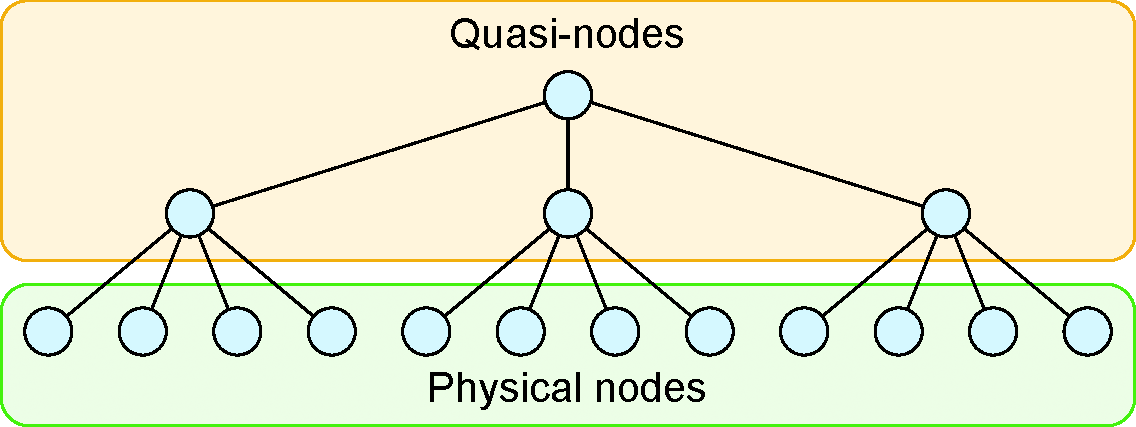
\includegraphics[width=\columnwidth]{figures/trust_hierarchy.pdf}
\caption{} \label{fig:trust_hierarchy}	
\end{figure}

\end{document}
